% %%%%%%%%%%%%%%%%%%%%%%%%%%%%%%%%%%%%%%%%%%%%%%%%%%%%%
% % Chapter 1. Introduction
% %%%%%%%%%%%%%%%%%%%%%%%%%%%%%%%%%%%%%%%%%%%%%%%%%%%%%
% \chapter{Introduction} \label{Ch:intro}

% 심혈관 질환(cardiovascular disease, CVD)은 전 세계적으로 가장 높은 사망 부담을 차지하는 질환군으로, 조기 진단과 지속적인 관리가 중요하다.
% 그 중 심장의 불규칙한 전기적 활동으로 발생하는 부정맥(arrhythmia)은 혈역학적 불안정, 심부전, 심정지 등 중증 합병증으로 이어질 수 있다.
% 특히 심방세동(atrial fibrillation, AFIB)은 대표적인 부정맥으로, 뇌졸중(stroke) 위험을 약 5배 증가시키는 것으로 보고되었다~\cite{wolf1991atrial}.
% 발작성(paroxysmal) 부정맥은 지속 시간이 짧고 간헐적으로 발생하므로, 약 10초 동안 정적으로 측정하는 standard 12-lead 심전도 검사만으로는 모든 에피소드를 포착하기에 한계가 있다.
% 이에 따라 임상에서는 Holter 및 wearable patch와 같은 장기 ECG 모니터링 장치를 이용하여 간헐적으로 발생하는 부정맥을 포착한다~\cite{steinhubl2018wearable}.

% 스마트워치 기반 불규칙 맥박 탐지와 후속 ECG patch 확인도 병원 밖 부정맥 탐지의 한 형태로 사용되며~\cite{perez2019large}, wearable patch를 이용한 연속 ECG 모니터링도 보고되어 있다~\cite{steinhubl2018wearable}.
% 이러한 웨어러블 장치는 사용자의 일상생활을 크게 제한하지 않으면서 심장 활동을 기록할 수 있으므로, 간헐적으로 발생하는 부정맥을 탐지하는 데 유용하다.
% 그러나 수일에서 수주에 걸쳐 축적되는 방대한 ECG를 의료진이 모두 수동으로 판독하는 것은 현실적으로 어려우며, 따라서 자동 ECG 분석 기술이 요구된다.

% 초기의 자동 ECG 분류 연구는 전통적인 신호처리 기법으로 ECG의 특징을 추출하였다.
% 심박 간격, QRS 폭 및 파형 진폭과 같은 delineation feature를 추출하거나 형태학적, 시간적 특징을 설계한 뒤 이를 기계학습 분류기에 입력하는 방식에 주로 의존하였다~\cite{de2004automatic,melgani2008classification,luz2016ecg,raj2017ecg}.
% 이후 심층신경망(deep neural network, DNN)은 이러한 특징 설계 과정을 data-driven 방식으로 end-to-end 최적화할 수 있다는 장점을 바탕으로 주류 기법으로 자리잡았다.
% 국소 형태학적 패턴 추출에 강점을 가지는 convolutional neural networks (CNNs)~\cite{niu2019inter,jing2021ecg}, 박동 간 시간적 의존성을 모델링하는 recurrent neural networks (RNNs)~\cite{saadatnejad2019lstm,hou2019lstm} 및 state space models (SSMs)~\cite{lee2025atrial,bathini2026mamba}, 그리고 시점 간 상관관계를 전역적으로 모델링하는 transformers~\cite{islam2024cat,che2021constrained} 등이 대표적이다.

% 그러나 학습 데이터에 대해 높은 정확도를 보이는 DNN 모델도 관찰하지 못한 새로운 환자에게 적용될 때 성능이 크게 저하될 수 있다~\cite{llamedo2011heartbeat,jeong2024enhancing}.
% ECG 파형은 심장의 해부학적 구조와 생리적 상태뿐만 아니라 연령, 성별, 기저질환, 전극 부착 위치 및 측정 장치의 특성에 따라서도 달라지기 때문이다.
% 그 결과 동일한 환자의 심박이 학습 및 평가 데이터에 모두 포함되는 환자 내(intra-patient) 환경에서는 높은 성능을 보이더라도, 학습 과정에서 관찰하지 못한 환자를 평가하는 환자 간(inter-patient) 환경에서는 성능이 저하된다.

% 이러한 변동성을 완화하기 위해 환자별 기준 정보를 모델에 반영하는 개인화(personalization) 기법~\cite{xu2019ivector, heo2026resumamba, fan2025class}이 제안되어 왔다.
% 개인화는 절대적인 파형 형태가 아니라 해당 환자의 기준 파형으로부터의 상대적 편차를 판별하도록 유도하여, 환자 간 형태학적 분산의 영향을 구조적으로 완화한다.
% 개인화 방식의 분류와 대상 모델의 위치는 Section~\ref{sec:bg_wearable}에서 정리한다.
% 기존 연구는 정확도 향상과 개인화 성능을 중심으로 평가하며,
% 정통적인 머신러닝 방법은 제외하고, 딥러닝 모델에서의 모바일 on-device 스트리밍 실행과 실제 기기 계측을 함께 다루는 연구는 상대적으로 제한적이다.
% 개인화 구조는 환자 특성을 추출하고 분류 특징에 결합하는 계산 경로를 포함한다.
% Mamba는 CUDA 가속 selective-scan 구현과 순수 PyTorch 참조 구현을 제공한다~\cite{gu2023mamba}.
% 본 논문에서는 모바일 CPU 배포를 위해 표준 ATen 연산 기반의 배포용 순차 scan을 사용한다.
% 웨어러블 및 모바일 플랫폼에서는 연속 ECG 입력을 심박 단위로 처리하면서
% 각 입력에 대한 계산을 지속적으로 수행할 수 있는지가 중요하다.
% 원시 ECG를 서버로 전송하는 cloud-based analysis는 통신 경로와 외부 계산 자원을 필요로 하며,
% on-device 분석은 스마트폰 내부에서 ECG 처리와 추론을 수행하는 구현 방식이다~\cite{park2024realtime,xu2026cardiolike}.
% 본 연구에서는 실시간 처리를 연속적으로 유입되는 ECG stream에 대해
% 심박 입력 구성과 분류 추론을 순차적으로 수행하는 것으로 정의하고,
% 모델 실행시간과 실제 streaming 처리시간을 측정한다.
% 본 논문에서는 inter-patient 일반화를 목표로 제안된 patient-conditioned ResUMamba~\cite{heo2026resumamba}를 대상 모델로 선정하고,
% 이를 스마트폰에서 심박 단위로 실행하기 위한 모델 경량화와 배포 방법을 구현한다.
% ResU path의 합성곱을 depthwise separable convolution으로 대체하여 모델 크기를 줄이고,
% Mamba path의 selective scan을 모바일 CPU 표준 런타임에서 실행 가능한 형태로 변환한다.
% 또한 HiCardi patch와 연동되는 스마트폰 애플리케이션을 구현하여
% ECG 수신부터 심박 단위 추론까지의 streaming 경로를 측정한다.
% 실험에서는 HiCardi dataset의 record-wise split에서 ResUMamba와 ResDSUMamba의 분류 성능을 비교하고,
% Galaxy~S21+에서 모델 실행시간과 실제 streaming 처리시간 및 자원 사용량을 측정한다.

% 본 논문의 기여는 다음과 같다.
% \begin{itemize}
% \item 기존 ResUMamba의 ResU path에 depthwise separable convolution (DSConv)을 적용하여 ResDSUMamba를 구성하고, HiCardi dataset에서 재학습한다.
% \item Mamba path의 selective scan을 PyTorch 표준 연산(ATen) 기반 순차 scan으로 구성하여 ExecuTorch와 XNNPACK backend에서 실행 가능한 형태로 변환하고, backend 구성에 따른 실행시간을 측정한다.
% \item HiCardi patch와 BLE로 연동되는 스마트폰 애플리케이션을 구현한다. 샘플 번호를 시간축으로 사용하고 원형 버퍼로 심박 구간을 구성하며, 수신과 추론을 서로 다른 스레드에서 처리한다.
% \item HiCardi dataset에서 두 모델의 분류 성능을 비교하고, 실제 스마트폰에서 모델 실행시간과 스트리밍 중 심박당 처리시간 및 자원 사용량을 측정한다.
% \end{itemize}


% \clearpage

% %%%%%%%%%%%%%%%%%%%%%%%%%%%%%%%%%%%%%%%%%%%%%%%%%%%%%
% % Chapter 2. Background and Related Works
% %%%%%%%%%%%%%%%%%%%%%%%%%%%%%%%%%%%%%%%%%%%%%%%%%%%%%
% \chapter{Background and Related Works} \label{ch:background}

% 본 장에서는 본 논문의 바탕이 되는 기존 연구를 정리한다.
% 먼저 웨어러블 ECG를 이용한 심박 단위 부정맥 분류와 환자 간 변동성 문제를 살펴보고, 대상 모델인 환자 조건화 ResUMamba의 구조를 설명한다.
% 이어서 부정맥 분류기의 임베디드·모바일 구현 연구를 소개하고,
% 마지막으로 모바일 DNN 배포 프레임워크와 selective scan의 배포 구현을 함께 다루며, selective scan을 병렬로 실행하는 방법이 단일 스레드 CPU에서 갖는 비용을 정리한다.

% %% =================================================
% \section{Inter-Patient Arrhythmia Classification from Wearable ECG} \label{sec:bg_wearable}

% Chapter~\ref{Ch:intro}에서 기술한 환자 간 변동성에 대응하는 방법은 크게 두 가지로 나뉜다.
% 하나는 환자와 관계없이 공통된 특징을 학습하는 일반화(generalization) 방식~\cite{de2004automatic,niu2019inter,jeong2024enhancing}이고,
% 다른 하나는 환자별 정보를 직접 활용하는 개인화(personalization) 방식이다.
% 개인화 방식 중 환자마다 분류기를 따로 학습하거나~\cite{llamedo2012automatic,de2006patient,fan2025class} 사전학습 모델을 환자 데이터로 fine-tuning하는 방식은 새로운 환자마다 라벨링과 추가 학습이 필요하다.
% 반면 화자 인식의 i-vector를 ECG에 적용한 방식~\cite{xu2019ivector}과 같이 환자를 대표하는 임베딩을 추출하여 분류기의 중간 특징에 결합하는 방식은 하나의 모델을 모든 환자가 공유하므로 배포에 유리하다.
% 특히 라벨 없는 환자 조건화(label-free patient conditioning)~\cite{heo2026resumamba}는 라벨 없는 환자의 기준 ECG로부터 임베딩을 추출하여 모델에 입력하므로, 배포 이후 추가 학습 없이 사용할 수 있어 웨어러블 환경에 적합하다.
% 본 논문의 대상 모델인 ResUMamba는 이 방식을 사용한 모델이다.

% %% =================================================
% \section{Patient-Conditioned ResUMamba} \label{sec:bg_resumamba}

% % --------------------------------------------------------------------
% \begin{figure}[t]
%     \centering
%     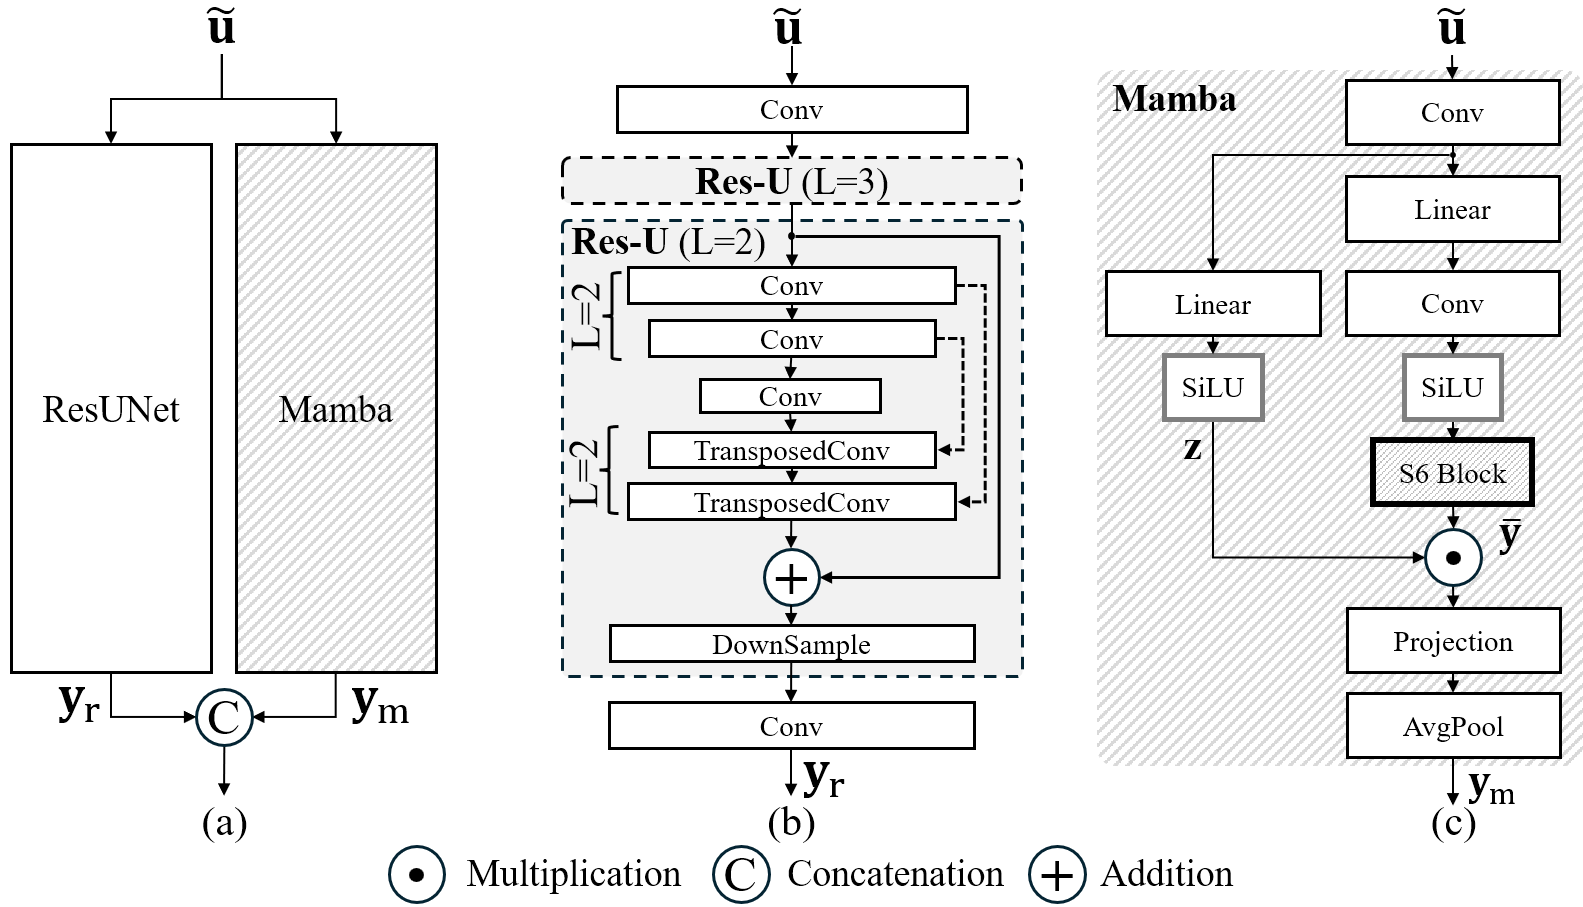
\includegraphics[width=\textwidth]{figures/ResUMamba.png}
%      \caption[Dual-path backbone of patient-conditioned ResUMamba~\cite{heo2026resumamba}.]{%
% Dual-path backbone of patient-conditioned ResUMamba~\cite{heo2026resumamba}.
% (a)~Parallel ResU and Mamba paths.
% (b)~ResU path with two cascaded Res-U blocks.
% (c)~Gated Mamba path with an S6 block.}
%     \label{fig:resumamba_arch}
% \end{figure}
% % --------------------------------------------------------------------

% 본 논문의 실시간 온디바이스 구현 대상은 환자 조건화 심박 분류를 위해 제안된 ResUMamba~\cite{heo2026resumamba}이다.
% Fig.~\ref{fig:resumamba_arch}(a)와 같이, R-peak 기준 심박 구간 $\tilde{\mathbf{u}}$는 ResU path와 Mamba path에 병렬로 들어간다.
% ResU path는 다중 해상도 합성곱으로 P파, QRS complex, T파의 형태를 표현하고, Mamba path는 selective state space model로 구간 안의 시간 의존성을 표현한다.
% 두 경로의 출력 $\mathbf{r}$, $\mathbf{m}$은 이어 붙여진 뒤 환자의 기준 ECG에서 얻은 환자 임베딩 벡터(patient embedding vector, PEV) $\mathbf{p}$로 조건화되고, RR 간격 등 임상 특징 $\mathbf{c}$와 결합되어 분류기로 전달된다.

% ResU path는 residual U-Net~\cite{ronneberger2015unet,zhang2018resunet}을 1차원 ECG에 맞춘 경로이다.
% Fig.~\ref{fig:resumamba_arch}(b)와 같이 입력 합성곱, 깊이 $L=3$과 $L=2$의 Res-U 블록, 출력 합성곱이 이어진다.
% 각 블록은 $L$번의 stride-2 합성곱으로 해상도를 줄였다가 transposed convolution과 skip connection으로 복원한 뒤, 블록 입력을 더하고(residual) 다시 해상도를 절반으로 줄인다.
% 이 경로는 표준 1차원 합성곱을 반복하므로, 모바일에서는 합성곱 연산량이 주된 실행 비용이 된다.

% Mamba path는 state space model (SSM)에 기초한다.
% SSM은 연속 시간 선형 시스템을 이산화하여 시퀀스 길이에 선형인 비용으로 상태를 갱신하며,
% S4 계열~\cite{gu2021s4,gu2022parameterization}을 거쳐 상태 전이 행렬을 대각 행렬로 두는 구조가 자리 잡았다.
% Mamba~\cite{gu2023mamba}는 이 대각 SSM의 이산화 간격과 입출력 벡터를 입력에 따라 바꾸어, 상태에 남길 정보를 선택하는 selective SSM (S6)을 도입하였다.
% ResUMamba는 Fig.~\ref{fig:resumamba_arch}(c)와 같이 입력 합성곱 뒤에 gating 분기(Linear--SiLU)와 주 분기(Linear--Conv--SiLU--S6)를 두고, 두 분기의 원소별 곱을 투영한 뒤 평균 pooling하여 $\mathbf{m}$을 얻는다.

% 입력 특징을 $\mathbf{x}_t\in\mathbb{R}^{D}$, 상태를 $\mathbf{H}_t\in\mathbb{R}^{D\times N}$이라 하면 S6는 다음과 같다.
% \begin{equation}
% \begin{aligned}
% \mathbf{H}_t &= \overline{\mathbf{A}}_t\odot\mathbf{H}_{t-1} + \mathbf{b}_t,
% \qquad \mathbf{b}_t=(\boldsymbol{\delta}_t\odot\mathbf{x}_t)\mathbf{B}_t^{\top}, \\
% \mathbf{y}_t &= \mathbf{H}_t\mathbf{C}_t + \mathbf{d}\odot\mathbf{x}_t.
% \end{aligned}
% \label{eq:selective_ssm}
% \end{equation}
% $\boldsymbol{\delta}_t\in\mathbb{R}^{D}$는 이산화 간격, $\mathbf{B}_t,\mathbf{C}_t\in\mathbb{R}^{N}$은 입력을 상태에 쓰고 상태에서 출력을 읽는 벡터이며, 셋 모두 $\mathbf{x}_t$에서 만들어진다.
% $\mathbf{A}\in\mathbb{R}^{D\times N}$은 채널별 대각 전이의 성분을 모은 양수의 고정 파라미터이며, 상태 갱신의 안정성을 보장하기 위해 실제 계산에서는 음수로 반전시켜 적용한다.
% 이에 따라 이산화된 전이는 $\overline{\mathbf{A}}_t=\exp(-\boldsymbol{\delta}_t\mathbf{1}_N^{\top}\odot\mathbf{A})$로 정의되며, $\mathbf{d}\in\mathbb{R}^{D}$는 skip 계수이다. $\boldsymbol{\delta}_t$는 softplus 연산을 통해 항상 양수로 유지되므로, 매개변수화된 $-\mathbf{A}$와 결합하여 상태의 각 성분이 자신의 감쇠 계수 $\overline{a}_t\in(0,1)$ 안에서 안정적으로 갱신됨을 보장한다.
% $\odot$은 원소별 곱이며, 길이 $T$에 대한 비용은 $\mathcal{O}(TDN)$이다.
% $\mathbf{H}_t$가 $\mathbf{H}_{t-1}$에 의존하므로 식~\eqref{eq:selective_ssm}을 그대로 계산하면 $T$번의 순차 단계가 필요하다.
% 이 순차성이 모바일 배포에서 문제가 되는 이유는 Section~\ref{sec:bg_scan}에서 다룬다.

% 환자 조건화에 쓰는 PEV $\mathbf{p}$는 라벨 없는 짧은 기준(calibration) ECG에서 얻는다.
% Contrastive predictive coding (CPC) 기반 자기지도학습으로 학습된 encoder가 이 구간의 잠재 특징을 고정 크기 벡터로 요약하며, 부정맥 정답을 쓰지 않으므로 새 환자에 대해 추가 라벨링이나 fine-tuning이 필요 없다.

% %% =================================================
% \section{Embedded and Mobile Arrhythmia Classifiers} \label{sec:bg_embedded}

% 부정맥 분류기를 웨어러블 또는 모바일 장치에서 실시간으로 실행하려는 연구는 CNN, RNN, CRNN 및 TCN 기반 모델을 중심으로 발전해 왔다.
% Kiranyaz 등~\cite{kiranyaz2016realtime}은 환자별로 학습한 1차원 CNN으로 심박을 실시간 분류하였다.
% Saadatnejad 등~\cite{saadatnejad2019lstm}은 wavelet 특징과 LSTM을 결합하여 개인용 웨어러블 장치에서의 연속 모니터링을 수행하였다.
% Faraone과 Delgado-Gonzalo~\cite{faraone2020crnn}는 convolutional-recurrent 모델을 Cortex-M4 기반 nRF52 SoC에서 실행하였으며,
% Ingolfsson 등~\cite{ingolfsson2021ecgtcn}은 temporal convolutional network를 마이크로컨트롤러에 탑재하여 추론 에너지와 실시간 제약을 평가하였다.
% Lee 등~\cite{lee2022compressed}은 ResNet과 MobileNet을 TensorFlow Lite로 압축하여 임베디드 웨어러블 장치에서 비교하였다.
% 상용 웨어러블 기기에서 수집한 실환경 ECG를 이용한 다중 label 부정맥 분류도 보고되었다~\cite{zheng2024hierarchical}.

% 최근에는 SSM 기반 ECG 모델과 edge-end inter-patient 분류기도 제안되고 있다~\cite{lee2025atrial,bathini2026mamba,xu2026cardiolike}.
% HiCardi를 이용한 실시간 ECG 서비스 모델은 스마트폰을 사용자 인터페이스와 데이터 전송 경로로 사용하고 서버에서 분석을 수행한다~\cite{park2024realtime}.
% 본 연구는 환자 조건화 ResUMamba를 대상으로 모델 경량화와 모바일 CPU 배포를 수행하고,
% BLE 수신, 버퍼링, R-peak 검출 및 심박 단위 추론을 포함하는 스트리밍 경로를 스마트폰에서 구현한다.


% %% =================================================
% \section{Mobile DNN Deployment and Selective Scan Implementations} \label{sec:bg_deployment} \label{sec:bg_scan}

% 학습된 DNN을 모바일 장치에서 실행하려면 학습 프레임워크의 모델을 대상 런타임이 실행할 수 있는 형태로 변환해야 한다.
% TensorFlow Lite~\cite{tflite}는 학습 그래프를 경량 flatbuffer 모델로 변환하여 모바일 인터프리터에서 실행하고, PyTorch 계열에서는 PyTorch Mobile을 거쳐 최근 \texttt{torch.export} 기반의 ExecuTorch~\cite{executorch}가 제공된다.
% ExecuTorch는 모델을 정적 연산 그래프로 변환(export)한 뒤, 지원되지 않는 연산을 기본 연산으로 분해(decomposition)하고 메모리 배치를 미리 계획하여 실행 파일로 만들며, Android와 iOS용 런타임을 제공한다.
% ONNX Runtime~\cite{onnxruntime} 역시 ONNX 형식으로 변환된 모델을 다양한 하드웨어 backend 위에서 실행한다.

% 실행 성능은 런타임뿐 아니라 실제 연산 커널과 backend의 구현에 크게 좌우된다.
% XNNPACK~\cite{xnnpack}은 ARM NEON~\cite{armneon} 등 아키텍처별 SIMD 명령어에 맞춘 최적화 커널, 연산 융합(operator fusion), 간접 참조 기반 합성곱~\cite{dukhan2019indirect} 등을 제공하는 모바일 CPU 연산 라이브러리로, TensorFlow Lite와 ExecuTorch 모두에서 CPU backend로 사용된다.
% ExecuTorch에서는 그래프의 일부를 이러한 backend로 넘겨 실행하는 것을 위임(delegation)이라 한다.
% 합성곱, 선형 계층, 행렬곱과 같이 XNNPACK이 지원하는 연산은 최적화된 커널로 실행하고, 위임되지 않은 연산은 ExecuTorch kernel path에서 실행한다. 본 연구에서는 portable kernel과 XNNPACK 구성을 비교한다. Portable kernel은 reference 성격의 구현이다.
% 따라서 모델 최적화 단계에서부터 대상 런타임이 효율적으로 지원하는 연산 위주로 그래프가 구성되도록 하는 것이 중요하다.

% 모델 자체를 경량화하는 일반적인 기법으로는 MobileNets가 모바일 CNN의 핵심 구성요소로 채택·대중화한 depthwise separable convolution~\cite{howard2017mobilenets}, 가중치와 활성값을 8비트 정수로 표현하는 양자화~\cite{jacob2018quantization}, 구조적 가지치기와 지식 증류~\cite{hinton2015distilling} 등이 있다.
% 그러나 SSM 계열 모델에서는 이러한 기법만으로 배포 문제가 해결되지 않는다.

% Mamba의 공식 저장소는 CUDA selective-scan 확장과 순수 PyTorch 기반 참조 경로를 제공한다~\cite{gu2023mamba}. 본 연구는 Android CPU 배포를 위해 식~\eqref{eq:selective_ssm}의 순환식을 표준 ATen 연산으로 표현한 배포용 순차 scan을 사용한다.
% 식~\eqref{eq:selective_ssm}의 순환식은 병렬 prefix scan으로도 계산할 수 있다.
% 예를 들어, Hillis--Steele scan은 단계 수가 $\lceil\log_2 T\rceil$로 줄지만 총 연산량은 순차 scan의 약 $\log_2 T$배로 늘고~\cite{hillis1986data,harris2007parallel}, Blelloch scan은 총 연산량은 $\mathcal{O}(T)$이나 상향·하향 두 번의 sweep 때문에 순차 단계 수가 $2\lceil\log_2 T\rceil$이다~\cite{blelloch1990prefix}.
% 단일 스레드에서는 각 단계 내부의 병렬성을 충분히 활용하기 어려우므로, 본 논문은 청크 기반 scan이나 전용 연산자와 비교하지 않고 PyTorch 표준 연산으로 순환식을 순차적으로 실행하는 구현을 선택하였다.
% 구체적인 구현은 Section~\ref{sec:opt_mamba}에서 기술한다. 본 구현은 기존 selective SSM의 순환식을 모바일 CPU에서 실행 가능한 표준 연산 그래프로 표현하는 배포 변환이다.

% 전용 커널로 배포 비용을 낮춘 연구도 있다.
% MambaLite-Micro~\cite{xu2025mambalite}는 이산화를 순환 안으로 융합하여 MCU에서 중간 텐서 크기를 $\mathcal{O}(DN)$으로 줄였다.
% XAMBA~\cite{das2025xamba}는 NPU에서 Mamba-2의 누적합(CumSum)과 합산(ReduceSum)을 행렬 연산으로 바꾸었다.
% 이들 연구가 MCU, NPU 또는 전용 연산자를 대상으로 하는 것과 달리, 본 논문은 전용 scan 연산자를 추가하지 않고 모바일 CPU에서 ExecuTorch 표준 연산과 XNNPACK backend만 사용한다.

% \clearpage

% %%%%%%%%%%%%%%%%%%%%%%%%%%%%%%%%%%%%%%%%%%%%%%%%%%%%%
% % Chapter 3. Model Optimization and Deployment
% %%%%%%%%%%%%%%%%%%%%%%%%%%%%%%%%%%%%%%%%%%%%%%%%%%%%%
% \chapter{Model Optimization and Deployment for On-Device Inference}
% \label{ch:optimization}

% 본 장에서는 ResUMamba를 스마트폰에서 실시간으로 실행하기 위한 모델 수준의 최적화와 배포 방법을 기술한다.
% 전체 시스템 구성은 Fig.~\ref{fig:overall_architecture}와 같다.
% Section~\ref{sec:opt_targets}에서 최적화 목표와 제약을 정하고, Section~\ref{sec:opt_resu}에서 ResU path에 depthwise separable convolution을 적용한다.
% Section~\ref{sec:opt_mamba}에서는 Mamba path의 selective scan을 모바일 런타임에서 실행 가능한 순차 scan으로 다시 작성한다.
% 환자 조건화, 임상 특징 결합, 분류기의 입출력과 학습 절차는 변경하지 않는다.

% \begin{figure*}[t]
%     \centering
%     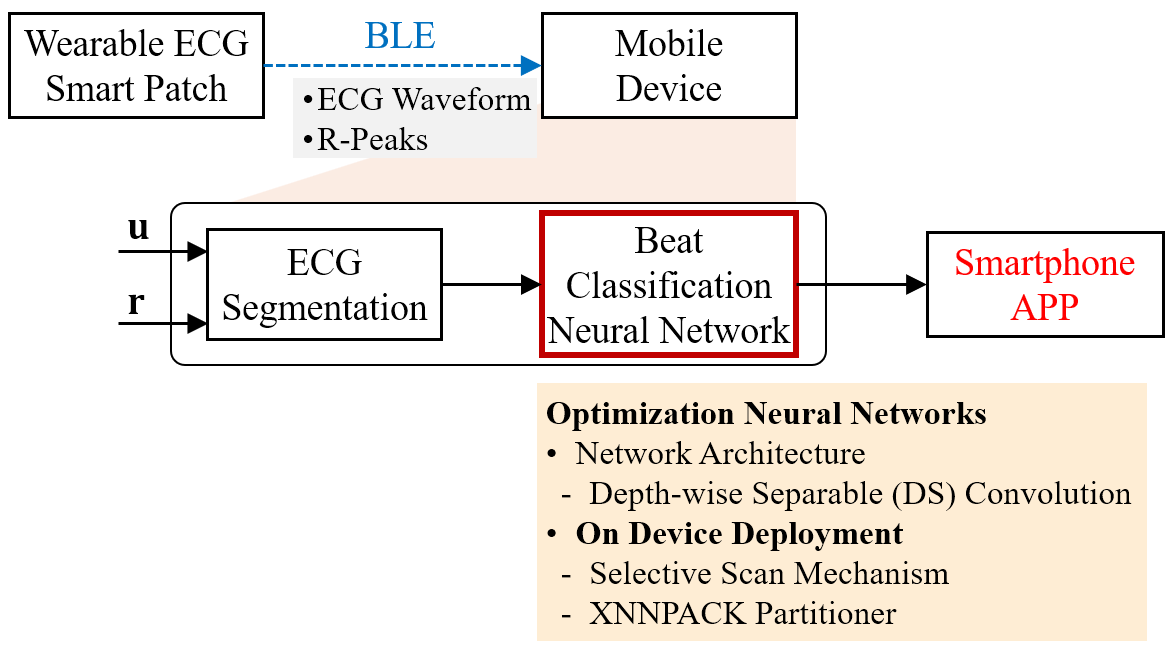
\includegraphics[width=0.95\textwidth]{figures/Overall Architecture.png}
%     \caption{Overall system architecture from wearable ECG acquisition to optimized on-device inference.}
%     \label{fig:overall_architecture}
% \end{figure*}

% %% =================================================
% \section{Optimization Targets and Constraints} \label{sec:opt_targets}

% 본 논문의 목표는 ResUMamba를 웨어러블 patch와 연동된 스마트폰에서 심박 단위로 실행하는 것이다.
% 이를 위해 모델의 파라미터 수와 MAC을 줄이고, 모바일 CPU에서의 실행시간을 측정한다.
% 준비된 심박 입력 하나에 대한 모델 forward의 CPU 실행시간을 $T_{\mathrm{model}}$로 정의하고 모델 수준의 주요 성능 지표로 사용한다.
% 실시간 streaming 환경에서는 각 심박 입력이 준비될 때마다 다음 입력이 누적되기 전에 처리를 완료할 수 있는지를 확인한다.
% 이를 위해 $T_{\mathrm{model}}$의 평균과 $P5$, $P50$, $P95$를 보고하고,
% 실제 streaming에서는 $T_{\mathrm{beat}}$와 $T_{\mathrm{queue}}$를 함께 측정한다.
% 본 시스템의 R-peak 검출기는 연속한 R-peak 사이의 최소 간격을 $240\,\mathrm{ms}$로 설정한다.

% ResU path는 표준 합성곱을 반복하므로 모델 계산량에서 큰 비중을 차지한다.
% 본 장에서는 이를 depthwise separable convolution으로 대체하여 모델의 계산량과 파라미터 수를 줄인다.
% ResDSUMamba는 동일한 HiCardi 분류 설정에서 재학습한다.
% Mamba path는 재학습된 ResDSUMamba의 가중치를 사용하고 export 단계에서 계산 표현을 ATen 연산 기반 순차 scan으로 변환한다.
% %% =============================================================================

% \section{ResU Path: Depthwise Separable Convolution}
% \label{sec:opt_resu}

% % --------------------------------------------------------------------
% \begin{figure}[t]
%     \centering
%     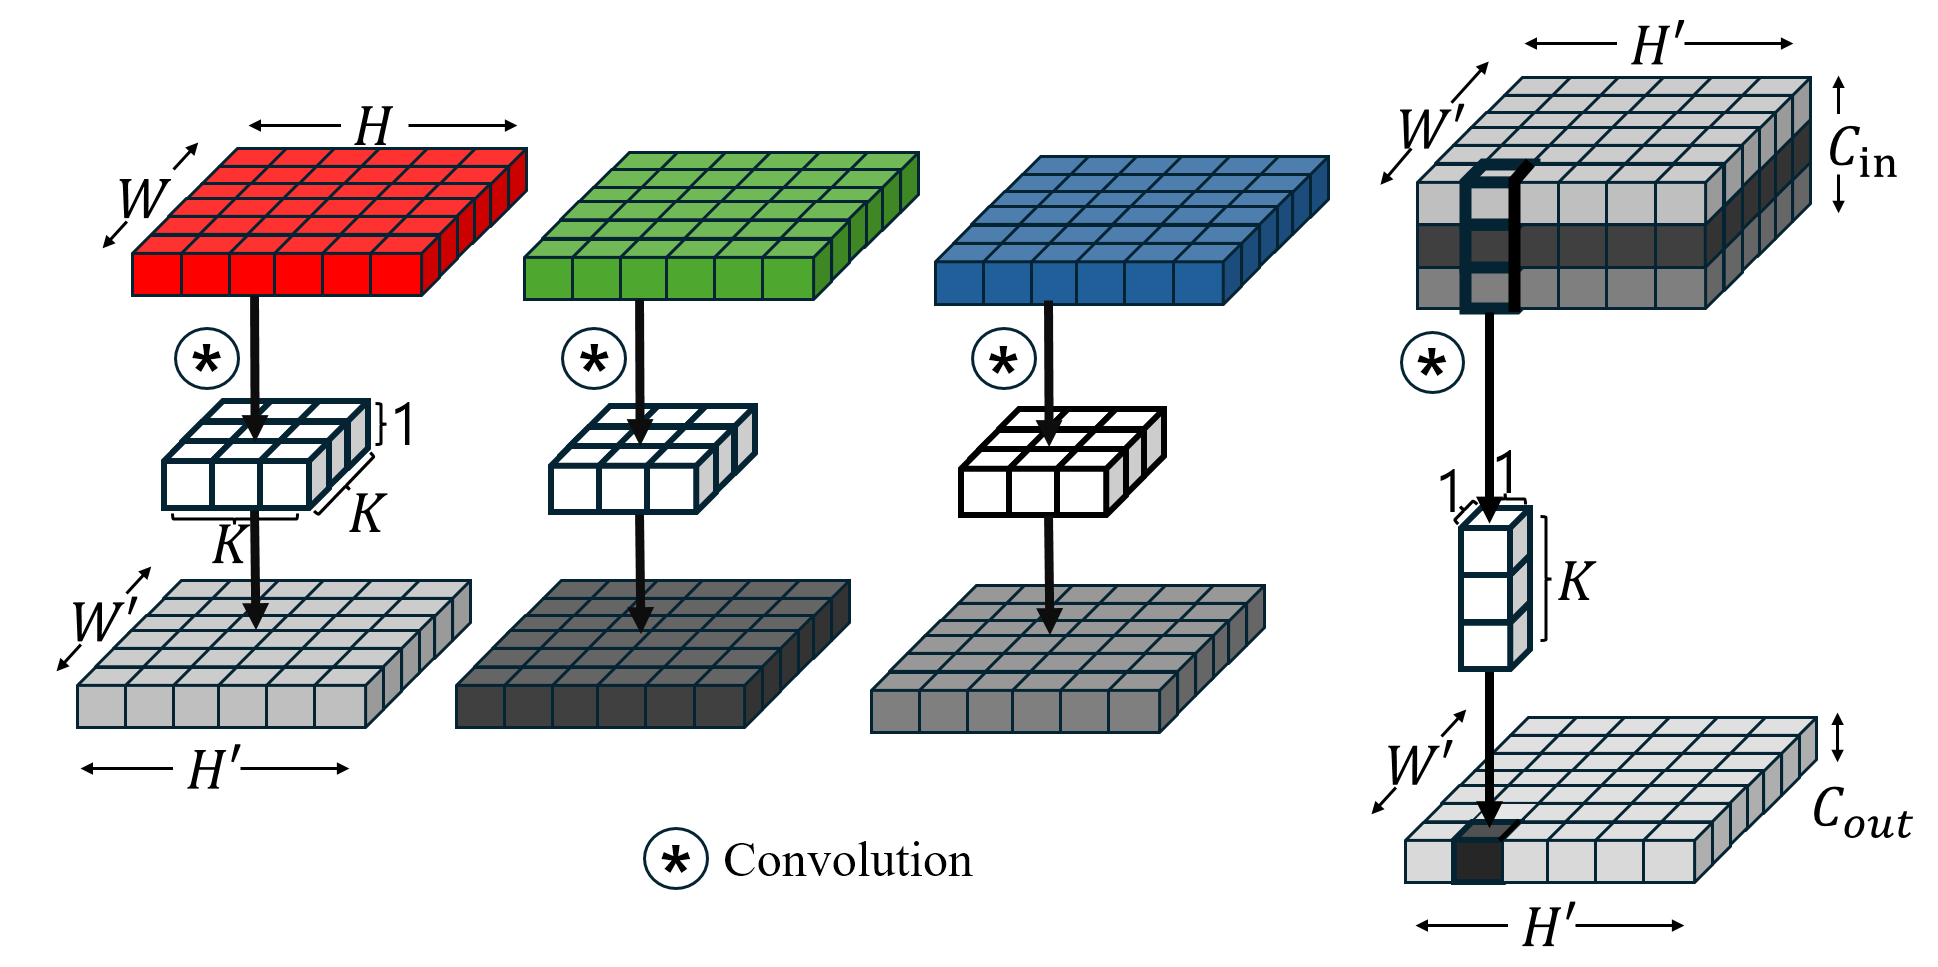
\includegraphics[width=\textwidth]{figures/dsconv.png}
%     \caption[Depthwise separable convolution~\cite{howard2017mobilenets}.]{%
% Depthwise separable convolution: independent channel-wise filtering followed by $1\times1$ pointwise convolution for channel mixing.}
%     \label{fig:dsconv}
% \end{figure}
% % --------------------------------------------------------------------

% Depthwise separable convolution (DSConv)~\cite{howard2017mobilenets}은 표준 합성곱이 동시에 수행하는 시간축 필터링과 채널 혼합을 두 단계로 분리한 연산이다.
% MobileNets는 이 구조를 모바일 비전 모델의 핵심 building block으로 채택하여 경량화를 대중화하였다.
% Fig.~\ref{fig:dsconv}와 같이 각 입력 채널에 독립적인 필터를 적용하는 depthwise convolution과, 커널 크기 $1$로 채널 간 정보를 결합하는 pointwise convolution으로 구성된다.

% 시간 $t$에서의 입력 및 출력 채널 벡터를 각각 $\mathbf{x}_t\in\mathbb{R}^{C_{\mathrm{in}}}$, $\mathbf{y}_t\in\mathbb{R}^{C_{\mathrm{out}}}$라 하면, 커널 크기가 $K$인 표준 1차원 합성곱은 다음과 같다.
% \begin{equation}
% \mathbf{y}_t = \sum_{k=0}^{K-1} \mathbf{W}_k\mathbf{x}_{t-k},\qquad
% \mathbf{W}_k\in\mathbb{R}^{C_{\mathrm{out}}\times C_{\mathrm{in}}}.
% \label{eq:standard_conv1d}
% \end{equation}
% 각 시점에서 크기 $C_{\mathrm{out}}\times C_{\mathrm{in}}$의 행렬-벡터 곱이 $K$번 수행되므로, 출력 길이를 $\tilde{T}$라 할 때 편향 항을 제외한 파라미터 수 $P_{\mathrm{conv}}$와 곱셈-누산(multiply-accumulate, MAC) 수 $M_{\mathrm{conv}}$는 다음과 같다.
% \begin{equation}
% P_{\mathrm{conv}} = K C_{\mathrm{in}} C_{\mathrm{out}},\qquad
% M_{\mathrm{conv}} = \tilde{T} K C_{\mathrm{in}} C_{\mathrm{out}}.
% \label{eq:conv_complexity}
% \end{equation}
% DSConv는 먼저 각 입력 채널에 대해 독립적인 $K$-tap 시간축 필터를 적용한다.
% \begin{equation}
% \mathbf{z}_t = \sum_{k=0}^{K-1} \mathbf{d}_k \odot \mathbf{x}_{t-k},\qquad
% \mathbf{d}_k \in \mathbb{R}^{C_{\mathrm{in}}},
% \label{eq:depthwise_conv1d}
% \end{equation}
% 여기서 $\odot$은 채널별 원소 곱이며, 채널 간 혼합은 수행하지 않는다.
% 이어서 pointwise convolution이 동일 시점의 채널 정보를 행렬 $\mathbf{P}$로 결합한다.
% \begin{equation}
% \mathbf{y}_t = \mathbf{P}\mathbf{z}_t,\qquad
% \mathbf{P}\in\mathbb{R}^{C_{\mathrm{out}}\times C_{\mathrm{in}}}.
% \label{eq:pointwise_conv1d}
% \end{equation}
% 따라서 DSConv의 파라미터 수와 MAC 수는 다음과 같다.
% \begin{equation}
% P_{\mathrm{DS}} = K C_{\mathrm{in}} + C_{\mathrm{in}}C_{\mathrm{out}},\qquad
% M_{\mathrm{DS}} = \tilde{T} \left(K C_{\mathrm{in}} + C_{\mathrm{in}}C_{\mathrm{out}} \right).
% \label{eq:dsconv_complexity}
% \end{equation}

% % --------------------------------------------------------------------
% \begin{figure}[t]
%     \centering
%     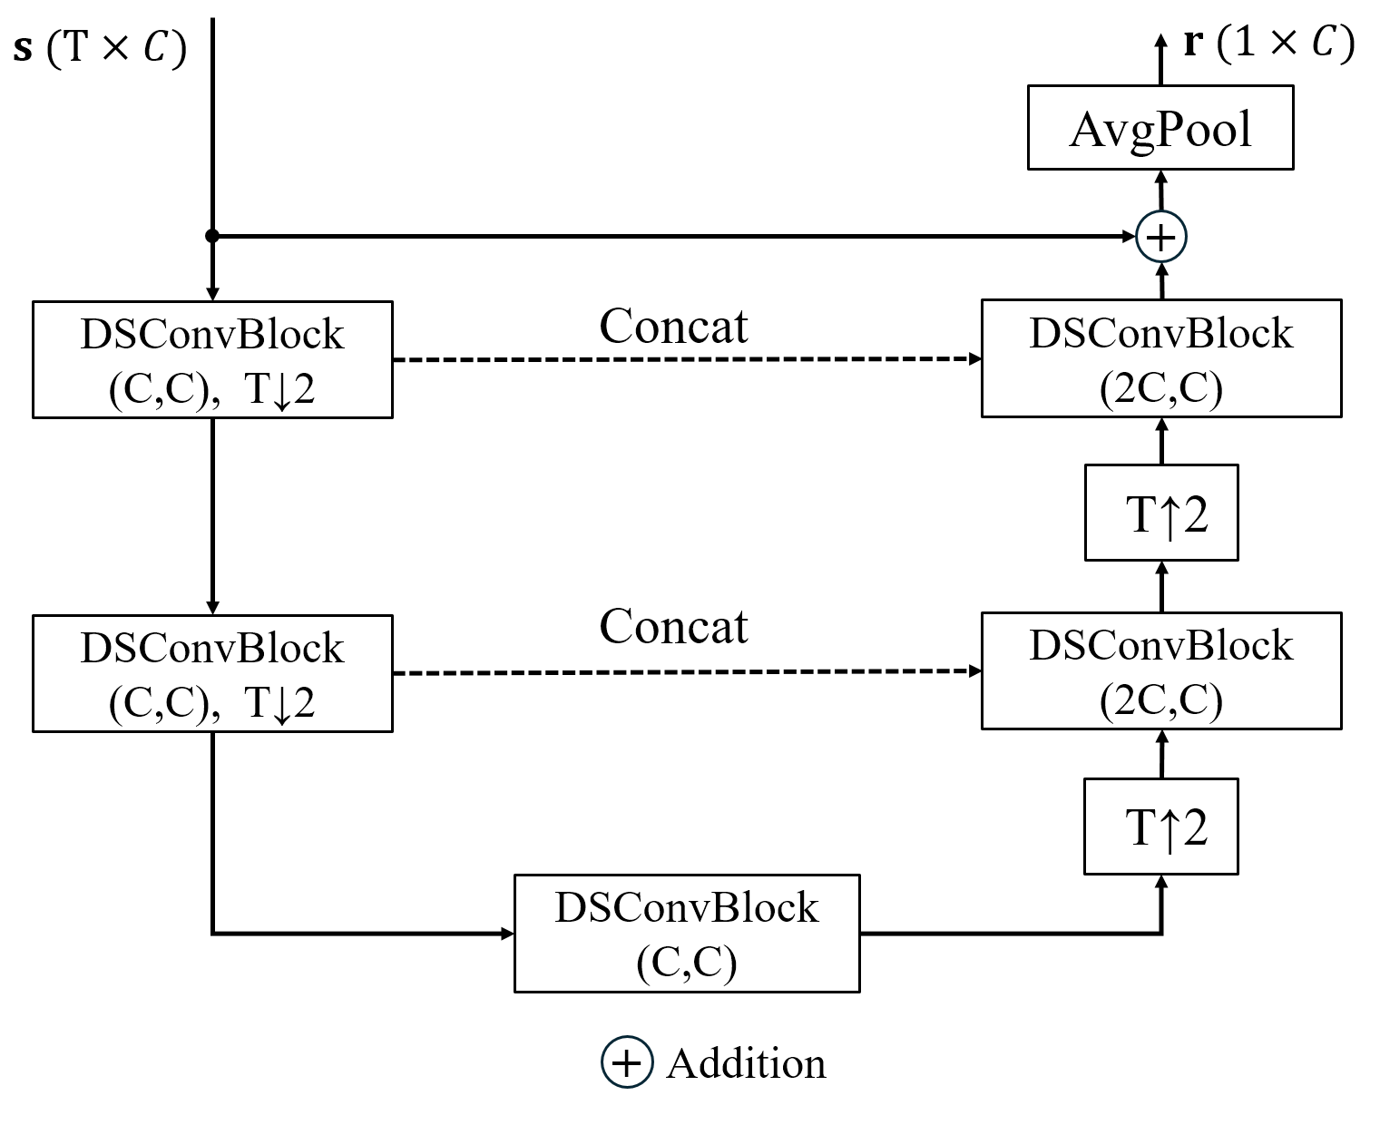
\includegraphics[width=\textwidth]{figures/ResDSUNet.png}
%     \caption[ResU path structure ($L=2$).]{%
% ResU path with encoder--decoder layer ($L=2$), skip connections, residual addition, and average pooling to produce $\mathbf{r}$.
% Decoding restores the length with parameter-free linear interpolation before the skip connection is concatenated; every convolution in the encoder, bottleneck and decoder blocks is a DSConv.}
%     \label{fig:resu_path}
% \end{figure}
% % --------------------------------------------------------------------

% 표준 합성곱 대비 상대 연산량은 $M_{\mathrm{DS}}/M_{\mathrm{conv}} = 1/C_{\mathrm{out}} + 1/K$이다.
% 본 논문에서는 Fig.~\ref{fig:resu_path}의 ResU path에 있는 합성곱을 DSConv로 대체하며, 이 경로의 합성곱은 $K=7$, $C_{\mathrm{out}}=128$이므로 합성곱 한 층의 이론적 감소율은 $1-(1/128+1/7)\approx84.9\%$이다.
% 대체 범위는 encoder block, bottleneck block 및 decoder block의 합성곱 전체이다.
% Decoding 단계에서 길이를 복원하는 보간은 학습 파라미터가 없는 선형 보간이므로 대체 대상이 아니며, 보간 이후 skip connection을 이어 붙인 뒤 수행되는 decoder block의 합성곱이 DSConv로 바뀐다.

% Table~\ref{tab:params_macs}는 입력 길이 $501$에서 두 모델의 모듈별 파라미터 수와 MAC 수를 정리한 것이다.
% MAC은 합성곱, 선형 계층, 행렬곱(배치 행렬곱 포함)과 attention의 곱셈-누산만 센 값이며, 정규화, 활성화 함수, scan의 원소별 상태 갱신($\overline{\mathbf{A}}_t\odot\mathbf{H}_{t-1}+\mathbf{b}_t$)과 같은 원소별 연산은 포함하지 않는다.
% ResU path의 MAC은 $490.27\,\mathrm{M}$에서 $100.15\,\mathrm{M}$으로 $79.6\%$ 감소하여 위의 층 단위 이론값 $84.9\%$보다 작다.
% 차이는 두 가지에서 온다.
% 첫째, 각 encoder 단의 downsampling은 두 모델 모두 이미 depthwise 합성곱과 pointwise 합성곱의 조합으로 구현되어 있어 대체 전후가 동일하다.
% 둘째, residual shortcut에서 채널 수를 맞추는 합성곱은 커널 크기가 $1$이므로 분해할 수 없고, decoder block의 첫 합성곱은 skip connection을 이어 붙인 $2C$ 채널을 입력으로 받아 $C_{\mathrm{in}}\neq C_{\mathrm{out}}$인 경우에 해당한다.
% Mamba path, 환자 조건화, 특징 결합 및 분류기는 변경하지 않았으므로, 모델 전체의 MAC 감소율은 $54.1\%$($721.50\,\mathrm{M}\rightarrow331.38\,\mathrm{M}$), 파라미터 감소율은 $46.9\%$($2.4883\,\mathrm{M}\rightarrow1.3225\,\mathrm{M}$)이다.

% \begin{table}[t]
% \centering
% \caption[Parameters and module-wise MACs.]{Parameters and module-wise MACs (input length $501$, batch $1$).
% Element-wise operations, including the scan state update, are excluded.
% Totals are the global counts, so they exceed the sum of the module rows by the matrix multiplications of the clinical cross-attention.}
% \label{tab:params_macs}
% \small
% \begin{tabular}{@{}lrrr@{}}
% \toprule
% Module & ResUMamba & ResDSUMamba & $\Delta$ \\
% \midrule
% \multicolumn{4}{@{}l}{MACs (M)} \\
% \quad input convolution        &   0.07 &   0.07 & -- \\
% \quad ResU path                       & 490.27 & 100.15 & $-79.6\%$ \\
% \quad Mamba path                      & 129.28 & 129.28 & -- \\
% \quad Patient conditioning            &   0.26 &   0.26 & -- \\
% \quad Fusion, classifier              &  98.78 &  98.78 & -- \\
% \quad Total                           & 721.50 & 331.38 & $-54.1\%$ \\
% \midrule
% \multicolumn{4}{@{}l}{Parameters (M)} \\
% \quad ㄴinput convolution        & 0.0004 & 0.0004 & -- \\
% \quad ResU path                       & 1.4787 & 0.3128 & $-78.8\%$ \\
% \quad Mamba path                      & 0.2653 & 0.2653 & -- \\
% \quad Patient conditioning            & 0.2632 & 0.2632 & -- \\
% \quad Fusion, classifier              & 0.4807 & 0.4807 & -- \\
% \quad Total                           & 2.4883 & 1.3225 & $-46.9\%$ \\
% \bottomrule
% \end{tabular}
% \end{table}

% Depthwise convolution은 연산량에 비해 메모리 접근량이 많아 연산 밀도(arithmetic intensity)가 낮으므로, 이론적 연산량 감소와 실제 실행시간 감소 사이에 차이가 발생할 수 있다.
% 또한 depthwise 합성곱과 pointwise 합성곱은 데이터 배치와 타일링이 서로 달라 범용 CPU 라이브러리에서 하나의 커널로 융합되지 않으며, 두 단계 사이에서 중간 텐서가 메모리에 실체화된다.
% 실제 단말에서의 실행시간 변화는 Section~\ref{subsec:exp_backend}에서 확인한다.

% %% =================================================
% \section{Mamba Path: Rewriting the Selective Scan for Mobile Deployment}
% \label{sec:opt_mamba}

% Mamba의 selective scan에는 CUDA로 가속되는 공식 경로가 존재하지만, selective SSM 자체는 표준 텐서 연산으로 표현할 수 있다~\cite{gu2023mamba}. Android CPU 배포에서는 CUDA 확장을 사용할 수 없으므로, 본 논문에서는 식~\eqref{eq:selective_ssm}의 순환을 PyTorch의 표준 ATen 연산으로 구성한 배포용 순차 scan을 사용하였다.
% DSConv 적용은 학습 단계에서 수행하고 selective scan 변환은 export 단계에서 수행한다. Export 단계에서는 학습된 가중치를 사용하며 계산 표현을 ATen 연산으로 변환한다. 이하 이 구현을 배포용 순차 scan이라 부른다.

% % --------------------------------------------------------------------
% \begin{figure}[t]
%     \centering
%     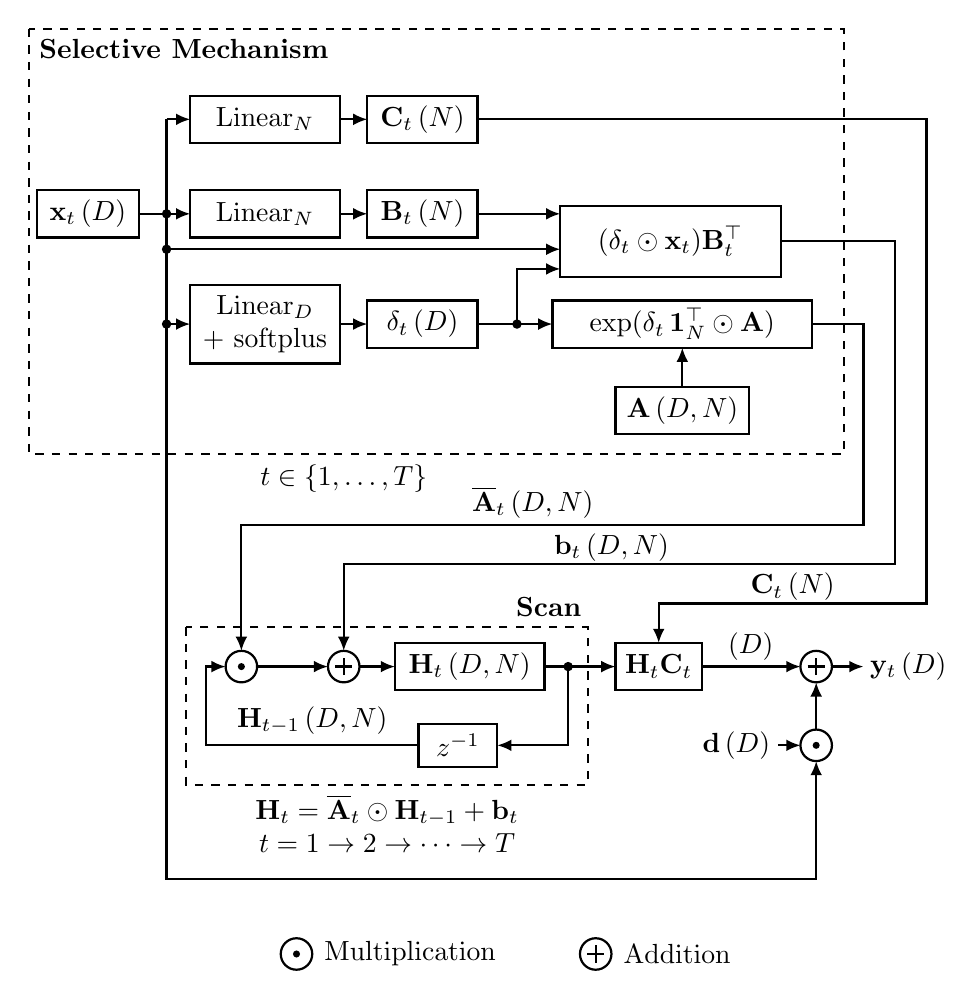
\begin{tikzpicture}[
    font=\normalsize,
    line width=0.8pt,
    arr/.style={-{Latex[length=1.8mm,width=1.5mm]}},
    blk/.style={draw,inner sep=1pt,align=center,minimum height=0.60cm},
    grp/.style={draw,dashed},
  ]
  % ---------------- Selective SSM (per-step computations) ----------------
  \draw[grp] (0.000,0.350) rectangle (10.350,-5.050);
  \node[anchor=north west,inner sep=2pt,align=left] at (0.050,0.300) {\textbf{Selective Mechanism}};
  \node[anchor=north,inner sep=2pt,align=center] at (4.000,-5.100) {$t\in\{1,\dots,T\}$};

  \node[blk,minimum width=1.30cm] at (0.750,-2.000) {$\mathbf{x}_{t}\,(D)$};
  \draw (1.400,-2.000) -- (1.750,-2.000);
  \draw (1.750,-0.800) -- (1.750,-3.400);
  \fill (1.750,-2.000) circle (0.06);
  \fill (1.750,-2.450) circle (0.06);
  \fill (1.750,-3.400) circle (0.06);
  \draw[arr] (1.750,-0.800) -- (2.050,-0.800);
  \draw[arr] (1.750,-2.000) -- (2.050,-2.000);
  \draw[arr] (1.750,-3.400) -- (2.050,-3.400);

  \node[blk,minimum width=1.90cm] at (3.000,-0.800) {Linear$_{N}$};
  \node[blk,minimum width=1.90cm] at (3.000,-2.000) {Linear$_{N}$};
  \node[blk,minimum width=1.90cm,minimum height=1.00cm] at (3.000,-3.400) {Linear$_{D}$\\+ softplus};
  \draw[arr] (3.950,-0.800) -- (4.300,-0.800);
  \draw[arr] (3.950,-2.000) -- (4.300,-2.000);
  \draw[arr] (3.950,-3.400) -- (4.300,-3.400);

  \node[blk,minimum width=1.40cm] at (5.000,-0.800) {$\mathbf{C}_{t}\,(N)$};
  \node[blk,minimum width=1.40cm] at (5.000,-2.000) {$\mathbf{B}_{t}\,(N)$};
  \node[blk,minimum width=1.40cm] at (5.000,-3.400) {$\boldsymbol{\delta}_{t}\,(D)$};

  \draw[arr] (5.700,-2.000) -- (6.750,-2.000);
  \draw[arr] (1.750,-2.450) -- (6.750,-2.450);
  \draw[arr] (5.700,-3.400) -- (6.650,-3.400);
  \fill (6.200,-3.400) circle (0.06);
  \draw[arr] (6.200,-3.400) -- (6.200,-2.700) -- (6.750,-2.700);

  \node[blk,minimum width=2.80cm,minimum height=0.90cm] at (8.150,-2.350) {$(\boldsymbol{\delta}_{t}\odot\mathbf{x}_{t})\mathbf{B}_{t}^{\top}$};
  \node[blk,minimum width=3.30cm] at (8.300,-3.400) {$\exp(\boldsymbol{\delta}_{t}\,\mathbf{1}_{N}^{\top}\odot\mathbf{A})$};
  \node[blk,minimum width=1.70cm] at (8.300,-4.500) {$\mathbf{A}\,(D,N)$};
  \draw[arr] (8.300,-4.200) -- (8.300,-3.700);

  % ---------------- outputs of the per-step part ----------------
  \draw[arr] (5.700,-0.800) -- (11.400,-0.800) -- (11.400,-6.950) -- (8.000,-6.950) -- (8.000,-7.450);
  \draw[arr] (9.550,-2.350) -- (11.000,-2.350) -- (11.000,-6.450) -- (4.000,-6.450) -- (4.000,-7.550);
  \draw[arr] (9.950,-3.400) -- (10.600,-3.400) -- (10.600,-5.950) -- (2.700,-5.950) -- (2.700,-7.550);
  \node[anchor=south,inner sep=2pt,align=center] at (6.400,-5.950) {$\overline{\mathbf{A}}_{t}\,(D,N)$};
  \node[anchor=south,inner sep=2pt,align=center] at (7.400,-6.500) {$\mathbf{b}_{t}\,(D,N)$};
  \node[anchor=south,inner sep=2pt,align=center] at (9.700,-7.00) {$\mathbf{C}_{t}\,(N)$};

  % ---------------- sequential scan ----------------
  \draw[grp] (2.000,-7.250) rectangle (7.100,-9.250);
  \node[anchor=south east,inner sep=2pt,align=right] at (7.100,-7.200) {\textbf{Scan}};
  \node[anchor=north,inner sep=2pt,align=center] at (4.550,-9.300) {$\mathbf{H}_{t}=\overline{\mathbf{A}}_{t}\odot\mathbf{H}_{t-1}+\mathbf{b}_{t}$\\$t=1\to2\to\cdots\to T$};

  % element-wise product: circle with a single dot (ISPLAB convention)
  \draw[fill=white] (2.700,-7.750) circle (0.2); \fill (2.700,-7.750) circle (0.045);
  % addition
  \draw[fill=white] (4.000,-7.750) circle (0.2); \draw (3.890,-7.750) -- (4.110,-7.750) (4.000,-7.860) -- (4.000,-7.640);
  \draw[arr] (2.900,-7.750) -- (3.800,-7.750);

  \node[blk,minimum width=1.90cm] at (5.600,-7.750) {$\mathbf{H}_{t}\,(D,N)$};
  \draw[arr] (4.200,-7.750) -- (4.650,-7.750);
  \fill (6.850,-7.750) circle (0.06);
  \draw[arr] (6.550,-7.750) -- (7.450,-7.750);
  \node[blk,minimum width=1.10cm] at (8.000,-7.750) {$\mathbf{H}_{t}\mathbf{C}_{t}$};

  \draw[arr] (6.850,-7.750) -- (6.850,-8.750) -- (5.950,-8.750);
  \node[blk,minimum width=1.00cm,minimum height=0.55cm] at (5.450,-8.750) {$z^{-1}$};
  \draw[arr] (4.950,-8.750) -- (2.250,-8.750) -- (2.250,-7.750) -- (2.500,-7.750);
  \node[anchor=south,inner sep=2pt,align=center] at (3.600,-8.700) {$\mathbf{H}_{t-1}\,(D,N)$};

  % ---------------- readout and skip ----------------
  \draw[arr] (8.550,-7.750) -- (9.800,-7.750);
  \node[anchor=south,inner sep=2pt,align=center] at (9.170,-7.750) {$(D)$};
  \draw[fill=white] (10.000,-7.750) circle (0.2); \draw (9.890,-7.750) -- (10.110,-7.750) (10.000,-7.860) -- (10.000,-7.640);
  \draw[arr] (10.200,-7.750) -- (10.600,-7.750);
  \node[anchor=west,inner sep=2pt,align=left] at (10.600,-7.750) {$\mathbf{y}_{t}\,(D)$};

  \draw[fill=white] (10.000,-8.750) circle (0.2); \fill (10.000,-8.750) circle (0.045);
  \draw[arr] (10.000,-8.550) -- (10.000,-7.950);
  \node[anchor=east,inner sep=2pt,align=right] at (9.500,-8.750) {$\mathbf{d}\,(D)$};
  \draw[arr] (9.520,-8.750) -- (9.800,-8.750);
  \draw[arr] (1.750,-3.400) -- (1.750,-10.450) -- (10.000,-10.450) -- (10.000,-8.950);
  

  % ---------------- Legend ----------------
  \draw[fill=white] (3.400,-11.400) circle (0.2); \fill (3.400,-11.400) circle (0.045);
  \node[anchor=west,inner sep=4pt] at (3.600,-11.400) {Multiplication}; % 이 부분 수정

  \draw[fill=white] (7.200,-11.400) circle (0.2); \draw (7.090,-11.400) -- (7.310,-11.400) (7.200,-11.510) -- (7.200,-11.290);
  \node[anchor=west,inner sep=4pt] at (7.400,-11.400) {Addition};

\end{tikzpicture}
%     \caption[Selective SSM of the Mamba path.]{Selective SSM of the Mamba path. All terms except the state update are computed independently at each step; only the state update is sequential. $z^{-1}$: one-step delay.}
%     \label{fig:ssm_block}
% \end{figure}
% % --------------------------------------------------------------------

% Fig.~\ref{fig:ssm_block}은 selective SSM의 계산 과정을 나타낸다.
% 입력 $\mathbf{x}_t$는 네 갈래로 나뉘어, 세 갈래에서 $\mathbf{B}_t$, $\mathbf{C}_t$, $\boldsymbol{\delta}_t$를 계산하고 나머지 한 갈래는 skip 항에 쓰인다.
% 이를 이용하여 $\overline{\mathbf{A}}_t$와 $\mathbf{b}_t$를 구성한다.
% 이 계산은 각 시점의 입력으로부터 독립적으로 수행할 수 있으므로 시퀀스 전체에 대해 먼저 계산할 수 있다.

% 따라서 순차 scan은 시퀀스 전체의 $\overline{\mathbf{A}}$와 $\mathbf{b}$를 먼저 계산한 뒤, 상태 갱신만 $t=1,2,\ldots,T$의 순서로 수행한다.
% Section~\ref{sec:bg_scan}에서 정리한 바와 같이 단일 스레드에서는 병렬 prefix scan의 이점이 없으므로, 본 논문은 이 순차 실행을 배포 구현으로 사용하였다.
% 입력 길이가 $T=501$로 고정되어 있으므로 \texttt{torch.export}는 이 반복문을 $501$개 시점으로 펼친(unrolled) 정적 그래프로 변환하며, 그래프는 PyTorch 표준 연산으로 구성된다.

% \clearpage

% %%%%%%%%%%%%%%%%%%%%%%%%%%%%%%%%%%%%%%%%%%%%%%%%%%%%%
% % Chapter 4. On-Device Real-Time Implementation
% %%%%%%%%%%%%%%%%%%%%%%%%%%%%%%%%%%%%%%%%%%%%%%%%%%%%%

% \chapter{On-Device Real-Time Implementation}
% \label{ch:implementation}

% \begin{figure}[t]
%   \centering
%   % fig_impl_overview.tex
% (a) HiCardi patch and electrode geometry, (b) system configuration.
% Requires: \usepackage{graphicx} only.
\begin{minipage}[b]{0.48\linewidth}
  \centering
  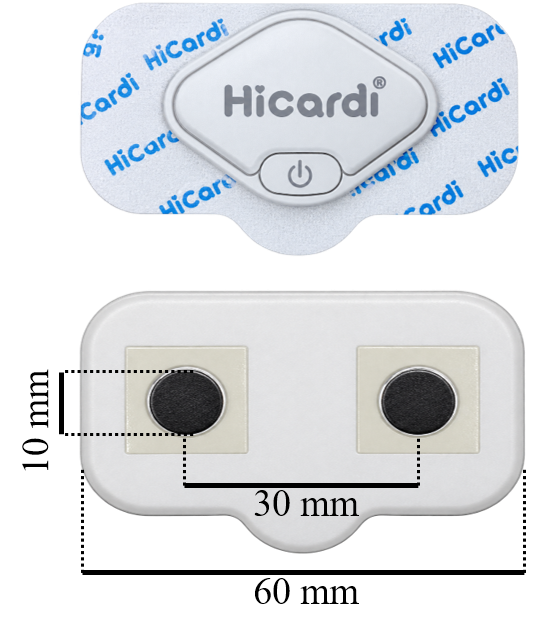
\includegraphics[height=80mm]{figures/impl_patch.png}\\[1.5mm]
  (a)
\end{minipage}%
\hfill
\begin{minipage}[b]{0.48\linewidth}
  \centering
  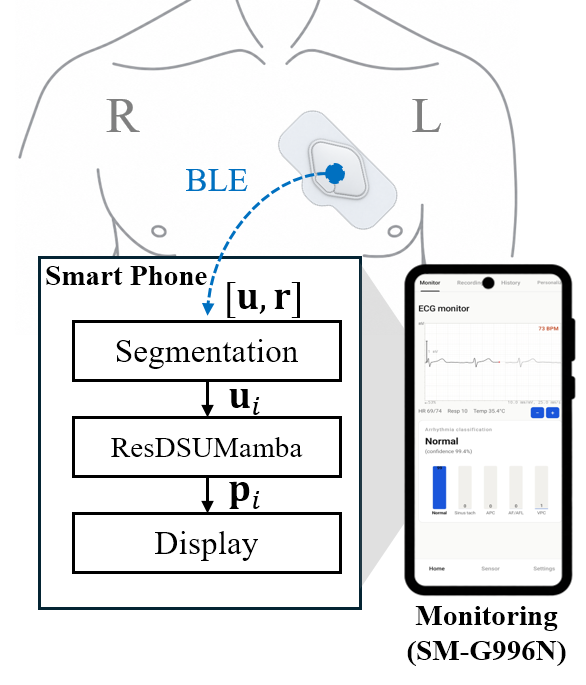
\includegraphics[height=80mm]{figures/impl_system.png}\\[1.5mm]
  (b)
\end{minipage}
%   \caption[HiCardi\textsuperscript{\textregistered} patch and system configuration.]{
%     HiCardi\textsuperscript{\textregistered} patch and system configuration.
%     (a) Patch and electrode geometry.
%     (b) ECG is streamed over BLE to the smartphone;
%     signal processing, beat classification, and display are performed on device.
%   }
%   \label{fig:impl_overview}
% \end{figure}

% Chapter~3에서 배포한 ResDSUMamba를 스마트폰 애플리케이션에 탑재하여
% HiCardi\textsuperscript{\textregistered}\textsuperscript{\textregistered} Smart Patch의 단일 유도 ECG를
% 연속적으로 수신하고 심박 단위로 처리하였다.
% 본 연구에서 실시간 처리는 연속 ECG stream에서 심박 입력을 순차적으로 구성하고
% 각 입력에 대한 추론과 결과 생성을 지속적으로 수행하는 방식으로 정의한다.
% Fig.~\ref{fig:impl_overview}와 같이 ECG는 패치에서 BLE로 전송되며,
% 신호 복원, R-peak 정렬, 입력 구성, 분류 및 결과 표시는 모두 스마트폰에서 수행된다.
% Fig.~\ref{fig:ble_spec}은 BLE notification의 프레임 구조와 ECG sample encoding을,
% Fig.~\ref{fig:impl_beat}은 수신된 샘플이 심박 단위 분류 결과로 이어지는
% 스마트폰 내부의 처리 흐름과 주요 상수를 나타낸다.

% % ====================================================
% \section{BLE Data Acquisition}
% % ====================================================

% 패치는 Nordic UART Service (NUS)~\cite{nus}를 통해 ECG를 전달한다.
% 측정 시작 시 스마트폰은 응답을 기다리지 않는 write without response 방식으로 시작 명령을 순차적으로 전송하며,
% 이후 패치는 42-byte notification으로 ECG를 주기적으로 전송한다.
% Fig.~\ref{fig:ble_spec}은 notification의 프레임 구조와 ECG sample encoding을 나타낸다.

% \begin{figure}[t]
%   \centering
%   % fig_impl_ble.tex
% BLE frame structure and ECG sample encoding.

\providecolor{bleblue}{RGB}{0,112,192}

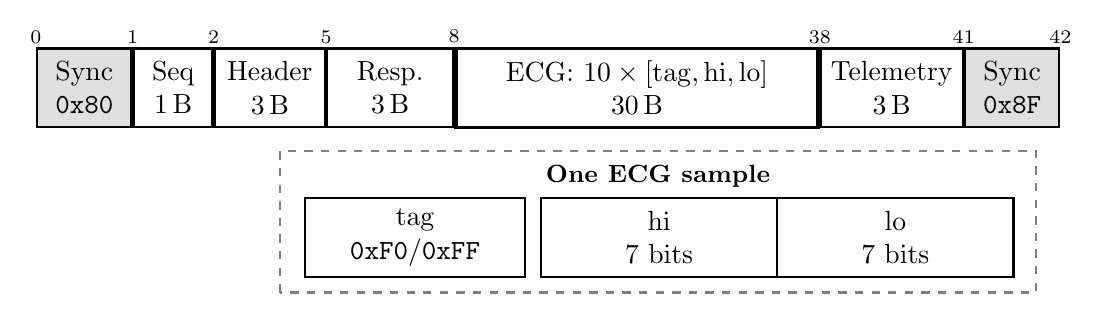
\begin{tikzpicture}[
  >=Stealth,
  thick,
  x=1mm,
  y=1mm,
  font=\rmfamily,
  cell/.style={
    draw,
    thick,
    minimum height=10mm,
    align=center,
    inner sep=1pt,
    anchor=west,
    font=\rmfamily
  },
  sync/.style={
    cell,
    fill=gray!25
  },
  sample/.style={
    draw,
    thick,
    minimum height=10mm,
    align=center,
    inner sep=2pt,
    anchor=west,
    font=\rmfamily
  },
  label/.style={
    anchor=south,
    font=\rmfamily\bfseries\small
  },
  off/.style={
    anchor=south,
    inner sep=1pt,
    font=\rmfamily\scriptsize
  },
  box/.style={
    draw=gray,
    thick,
    dashed,
    inner sep=3mm
  }
]

% 42-byte notification frame
\node[sync, minimum width=12mm] (c0) at (0,0)
  {Sync\\\texttt{0x80}};
\node[cell, minimum width=10mm] (c1) at (c0.east)
  {Seq\\1\,B};
\node[cell, minimum width=14mm] (c2) at (c1.east)
  {Header\\3\,B};
\node[cell, minimum width=16mm] (c3) at (c2.east)
  {Resp.\\3\,B};
\node[cell, minimum width=46mm, very thick] (c4) at (c3.east)
  {ECG: $10\times[\mathrm{tag},\mathrm{hi},\mathrm{lo}]$\\30\,B};
\node[cell, minimum width=18mm] (c5) at (c4.east)
  {Telemetry\\3\,B};
\node[sync, minimum width=12mm] (c6) at (c5.east)
  {Sync\\\texttt{0x8F}};

% Byte offsets
\foreach \c/\o in {
  c0/0,
  c1/1,
  c2/2,
  c3/5,
  c4/8,
  c5/38,
  c6/41
}{
  \node[off] at (\c.north west) {\o};
}
\node[off] at (c6.north east) {42};

% One ECG sample
\node[sample, minimum width=28mm] (tag) at (34,-19)
  {tag\\\texttt{0xF0}/\texttt{0xFF}};
\node[sample, minimum width=30mm] (hi) at (64,-19)
  {hi\\7 bits};
\node[sample, minimum width=30mm] (lo) at (94,-19)
  {lo\\7 bits};

% 점선 회색 박스와 라벨
\draw[box] (31,-26) rectangle (127,-8);
\node[label] at (79,-14) {One ECG sample};

\end{tikzpicture}
%   \caption[BLE frame structure and ECG sample encoding.]{
%     BLE frame structure and ECG sample encoding.
%     Each 42-byte notification contains 10 ECG samples represented by
%     \texttt{[tag, hi, lo]}, where \texttt{hi} and \texttt{lo} are 7-bit fields.
%   }
%   \label{fig:ble_spec}
% \end{figure}

% ECG 영역은 \texttt{[tag, hi, lo]}의 3-byte 묶음으로 구성되며,
% 각 42-byte notification에는 10개의 ECG sample이 포함된다.
% ECG tag를 확인한 묶음만 sample 복원에 사용하며,
% \texttt{hi}와 \texttt{lo}의 7-bit 데이터를 결합하여 14-bit ADC 값을 얻는다.

% \begin{equation}
%  v=(\texttt{hi}\,\&\,\texttt{0x7F})\,2^7
%  +(\texttt{lo}\,\&\,\texttt{0x7F}).
%  \label{eq:ble_decode}
% \end{equation}

% 복원된 ADC 값은 $x=(v-8192)/1000$으로 mV로 환산하며,
% 학습 데이터와 동일한 척도의 신호를 모델 입력으로 사용한다.

% 프레임의 유효 sample 상태는 연속적인 품질 조건으로 관리하며,
% 설정된 손상 sample 비율과 연속 프레임 조건에 따라 lead-off 상태를 판정한다.
% Lead-off 구간에서는 ECG waveform 표시와 기록을 유지하고
% R-peak 추적 및 추론 상태를 함께 관리한다.

% ECG의 signal time은 BLE notification의 도착 시각이 아니라 sample index를 기준으로 구성하며,
% sampling frequency는 $f_s=250\,\mathrm{Hz}$이다.
% RR 간격은 R-peak 사이의 sample index 차이로 계산하고,
% 패킷 sequence 정보는 수신 순서와 손실 구간을 확인하는 데 사용한다.

% %
% % ====================================================
% \section{On-Device Processing}
% \label{sec:impl_pipeline}
% % ====================================================

% \begin{figure}[t]
%   \centering
%   \providecolor{bleblue}{RGB}{0,112,192}
\usetikzlibrary{arrows.meta}

\begin{tikzpicture}[
  x=1mm,
  y=1mm,
  font=\rmfamily,
  >={Bar[width=0.8pt] Triangle[length=3pt,width=4pt]},
  blk/.style={
    draw, 
    thick, 
    align=center, 
    text width=32mm,
    minimum height=14mm, 
    inner sep=1.5pt, 
    anchor=north, 
    font=\rmfamily
  },
  head/.style={
    align=center, 
    anchor=north, 
    font=\rmfamily\bfseries
  },
  arr/.style={
    ->, 
    thick
  },
  ble/.style={
    ->, 
    thick, 
    densely dashed, 
    bleblue
  }
]

  % ==================================================
  % Headers
  % ==================================================
  \node[head] at (19, 0)  {BLE Callback};
  \node[head] at (57, 0)  {Receive};
  \node[head] at (95, 0)  {Inference};

  % ==================================================
  % BLE Callback
  % ==================================================
  \node[blk] (a1) at (19,-10) {Frame Check};
  \node[blk] (a2) at (19,-28) {ECG Decode\\{\scriptsize 14-bit samples}};
  \node[blk] (a3) at (19,-46) {Lead-off Detection};

  % ==================================================
  % Receive
  % ==================================================
  \node[blk] (b1) at (57,-10) {R-Flag Reception};
  \node[blk] (b2) at (57,-28) {R-Peak Alignment\\{\scriptsize Past buffer search}};
  \node[blk] (b3) at (57,-46) {Heart Rate Update};

  % ==================================================
  % Inference
  % ==================================================
  \node[blk] (c1) at (95,-10) {Ring Buffer};
  \node[blk] (c2) at (95,-28) {Beat Windowing\\{\scriptsize $r_k \pm 250$ samples}};
  \node[blk] (c3) at (95,-46) {ResDSUMamba\\{\scriptsize Classification}};
  \node[blk] (c4) at (95,-64) {Post-processing\\{\scriptsize Threshold}};

  % ==================================================
  % UI
  % ==================================================
  \node[head] at (19,-84) {UI};
  \node[blk] (d1) at (57,-84) {ECG Waveform\\{\scriptsize Real-time sweep}};
  \node[blk] (d2) at (95,-84) {Display Results\\{\scriptsize HR \& Labels}};

  % ==================================================
  % BLE input
  % ==================================================
  \draw[ble] (19,-5.7) -- (a1.north);
  \node[anchor=west, font=\rmfamily\scriptsize] at (18,-6.5) {BLE};

  % ==================================================
  % Internal flows 
  % ==================================================
  \foreach \s/\t in {a1/a2, a2/a3, b1/b2, b2/b3, c1/c2, c2/c3, c3/c4} 
    \draw[arr] (\s.south) -- (\t.north);

  % ==================================================
  % Cross-column flows
  % ==================================================
  \draw[arr] (a2.east) -- (36.5,-35) -- (36.5,-17) -- (b1.west);
  \draw[arr] (b2.east) -- (74.5,-35) -- (74.5,-17) -- (c1.west);

  % ==================================================
  % UI flows
  % ==================================================
  \draw[arr] (b3.south) -- (d1.north);
  \draw[arr] (c4.south) -- (d2.north);

  % ==================================================
  % Separators
  % ==================================================
  \foreach \x in {38, 76}
    \draw[gray!55, densely dashed, thin] (\x, 8) -- (\x, -75);

  \draw[gray!55, densely dashed, thin] (0, -78) -- (113, -78);

\end{tikzpicture}
%   \caption[End-to-end on-device beat processing.]{
%     End-to-end on-device beat processing.
%     The four columns are smartphone-side execution contexts,
%     and each box indicates the operation and its implementation constants.
%   }
%   \label{fig:impl_beat}
% \end{figure}

% Fig.~\ref{fig:impl_beat}과 같이 스마트폰의 처리는
% BLE callback, receive executor, inference executor 및 UI thread로 구성된다.
% BLE callback은 frame 검사와 sample 복원을 수행하고,
% receive executor는 R-peak 위치 보정과 심박 관련 정보를 관리한다.
% Inference executor는 심박 입력 구성, 임상 특징 계산, 모델 실행 및 결과 처리를 수행하며,
% UI thread는 ECG waveform과 심박 분류 결과를 갱신한다.
% Receive executor와 inference executor는 각각 단일 스레드로 동작하며,
% 스레드 간 데이터 전달에는 thread-safe queue를 사용한다.

% 복원된 mV sample은 sample index와 함께 고정 크기 원형 버퍼에 저장한다.
% 확정된 R-peak $r_k$를 기준으로
% $W_{\mathrm{pre}}=250$ samples와
% $W_{\mathrm{post}}=250$ samples를 사용하여
% $[r_k-W_{\mathrm{pre}}, r_k+W_{\mathrm{post}}]$ 구간의
% 501개 sample을 심박 입력으로 구성한다.
% R-peak 정렬과 beat window 구성에는 동일한 sample index를 사용한다.

% 패치의 R-peak tag는 실제 QRS보다 $\Delta_{\mathrm{tag}}$만큼 늦게 도착한다.
% 따라서 tag에 대응하는 과거 ECG 구간에서 QRS 위치를 탐색하여
% R-peak $r_k$를 결정한다.
% 연속한 R-peak 사이의 최소 간격은 $240\,\mathrm{ms}$로 설정한다.

% 학습 모델은 patient embedding과 rhythm-level clinical features를 함께 사용한다.
% Patient embedding $p\in\mathbb{R}^{256}$은 각 대상자의 초기
% $60\,\mathrm{s}$ 기준 ECG에서 CPC encoder를 이용하여 생성한다.
% Clinical feature vector $c\in\mathbb{R}^{32}$는 심박 및 rhythm 정보를 반영한다.
% Post-RR 정보는 현재 R-peak와 다음 R-peak 사이의 간격으로 계산한다.

% Beat 입력을 구성하려면 다음 R-peak의 확정과
% $W_{\mathrm{post}}$ samples의 미래 ECG 확보가 모두 필요하다.
% 따라서 입력 준비 시점은 두 조건 중 더 늦게 만족되는 시점으로 결정한다.
% R-peak tag의 지연과 미래 ECG sample 확보를 고려한
% beat $k$의 input waiting delay $D_k$는 다음과 같이 정의한다.

% \begin{equation}
% D_k=
% \max\!\left(
% RR_k^{\mathrm{post}}+\Delta_{\mathrm{tag}},
% \frac{W_{\mathrm{post}}}{f_s}
% \right).
% \label{eq:input_wait}
% \end{equation}

% 여기서 $RR_k^{\mathrm{post}}$는 현재 R-peak와 다음 R-peak 사이의 시간 간격이다.
% 본 구현에서는
% $W_{\mathrm{post}}=250$ samples,
% $f_s=250\,\mathrm{Hz}$,
% $\Delta_{\mathrm{tag}}=340\,\mathrm{ms}$를 사용한다.
% 평균 심박수 $80.2\,\mathrm{bpm}$을 기준으로 평균 RR 간격은 약
% $748\,\mathrm{ms}$이며,
% $RR_k^{\mathrm{post}}+\Delta_{\mathrm{tag}}$는 약 $1.088\,\mathrm{s}$이다.
% 또한 $W_{\mathrm{post}}/f_s=1.0\,\mathrm{s}$이므로,
% 이 조건에서 $D_k$는 약 $1.088\,\mathrm{s}$이다.
% 이 값은 모델 실행시간과 구분되는 입력 대기시간이다.

% 입력이 준비되면 501-sample ECG $x$,
% patient embedding $p$ 및 clinical feature vector $c$를
% ResDSUMamba에 입력한다.
% 각 label logit에는 sigmoid를 적용하여 label별 확률을 계산하고,
% 확률이 $0.5$ 이상인 label을 해당 beat의 분류 결과로 표시한다.
% ECG waveform은 실시간으로 갱신하며,
% 화면에는 HR, label별 확률, BLE connection 및 lead-off 상태를 표시한다.

% 실제 스트리밍에서는 입력이 준비된 심박을
% inference executor의 queue에 전달하고,
% inference executor는 queue 순서에 따라 심박 입력을 처리한다.
% 입력 준비 후 inference executor가 처리를 시작할 때까지의 시간은
% $T_{\mathrm{queue}}$로 측정하고,
% 입력 준비부터 결과 생성까지의 전체 경과시간은
% $T_{\mathrm{beat}}$로 측정한다.
% Chapter~\ref{ch:experiments}에서는 이를 모델 수준의
% $T_{\mathrm{model}}$과 구분하여 측정한다.


% %%%%%%%%%%%%%%%%%%%%%%%%%%%%%%%%%%%%%%%%%%%%%%%%%%%%%
% % Chapter 5. Experiments and Results
% %%%%%%%%%%%%%%%%%%%%%%%%%%%%%%%%%%%%%%%%%%%%%%%%%%%%%

% \chapter{Experimental Setup and Results}
% \label{ch:experiments}

% 본 장에서는 실험 설정과 Galaxy~S21+에서의 측정 결과를 보고한다.
% Section~\ref{sec:exp_setup}에서 데이터셋, 대상 단말, 시간 지표와 평가 지표를 정리하고,
% Section~\ref{sec:exp_model}에서 두 모델의 분류 성능과 XNNPACK 적용 여부에 따른 $T_{\mathrm{model}}$을 비교한다.
% Section~\ref{sec:exp_live}에서는 patch와 연동한 실제 스트리밍 환경에서의 처리시간과 자원 사용량을 제시한다.

% \section{Experimental Setup} \label{sec:exp_setup}
% % \subsection{HiCardi\textsuperscript{\textregistered} Dataset and } \label{subsec:exp_dataset}

% % HiCardi\textsuperscript{\textregistered} 데이터셋은 MEZOO Co., Ltd.의 HiCardi\textsuperscript{\textregistered} Smart Patch를 이용하여 수집한
% % 장시간 ECG 기록으로, 동잡음, 신호 손실 및 전극 접촉 상태 변화 등 실제 모니터링 환경에서 발생할 수 있는 신호 특성을 포함한다.
% % 전체 원자료는 Local Clinic, Kosin University Gospel Hospital 및
% % Yonsei University 관련 코호트 등 여러 수집 코호트로 구성되어 있으며,
% % 본 연구에서는 연구 목적에 맞는 기록을 선별하여 총 $8$개 코호트,
% % $203$명의 대상자로부터 수집된 $275$개 ECG record를 분석에 사용하였다.
% % 각 기록의 길이는 $0.03$--$47.5$시간이며, 단일 채널 ECG를
% % $250\,\mathrm{Hz}$로 표본화하였다.

% % 평가에는 Normal, APC, VPC, sinus tachycardia, AF/AFL의
% % 다섯 개 label을 사용하였다.
% % APC와 VPC는 심박 단위 형태 label이고, sinus tachycardia와 AF/AFL은
% % 구간 단위 리듬 label이다.
% % 하나의 심박 또는 구간은 둘 이상의 label을 가질 수 있는 multi-label 구성으로 처리하였다.
% % Normal은 정상 심박을 나타내는 기준 label로 포함하였다.

% % \begin{table}[h]
% % \centering
% % \caption[Record-wise split of the HiCardi\textsuperscript{\textregistered} dataset.]{Record-wise split and per-label beat counts of the HiCardi\textsuperscript{\textregistered} dataset (multi-label; counts do not sum to the total).}
% % \label{tab:HiCardi\textsuperscript{\textregistered}_split}
% % \resizebox{\textwidth}{!}{%
% % \begin{tabular}{lrrrrrrr}
% % \toprule
% % Subset & Records & Normal & Sinus~tachy. & APC & AF/AFL & VPC & Total beats \\
% % \midrule
% % Training   & 104 &   688\,735 & 49\,688 & 18\,647 &   391\,891 & 42\,831 & 1\,189\,357 \\
% % Validation &  33 &   101\,148 &  6\,026 & 21\,820 &   157\,855 &  3\,547 &   290\,297 \\
% % Test       & 138 & 7\,454\,184 & 58\,988 & 82\,491 & 1\,154\,790 & 35\,642 & 8\,777\,480 \\
% % \bottomrule
% % \end{tabular}}
% % \end{table}

% % Table~\ref{tab:HiCardi\textsuperscript{\textregistered}_split}에서 전체 beat 수 대비 train/validation/test의 비중은 각각 약
% % $11.6\%$, $2.8\%$, $85.6\%$이다.
% % 전체 beat 수 기준으로 test subset의 Normal과 AF/AFL은 각각 약 $84.9\%$와 $13.2\%$를 차지한다.
% % Micro 지표는 다수 label의 영향을 받으므로 Macro 지표와 함께 보고한다.



% \subsection{HiCardi\textsuperscript{\textregistered} Dataset}
% \label{subsec:exp_dataset}

% HiCardi\textsuperscript{\textregistered} 데이터셋은 MEZOO Co., Ltd.의 HiCardi\textsuperscript{\textregistered} Smart Patch로 수집한 장시간 ECG 기록이며, 동잡음, 신호 손실 및 전극 접촉 상태 변화 등 실제 웨어러블 모니터링 환경에서 발생하는 신호 특성을 포함한다.
% 단일 채널 ECG를 $250\,\mathrm{Hz}$로 표본화하였고, 기록 길이는 $0.03$--$47.5$시간이다.
% 기록은 $6$개 코호트의 $317$개이며, 이 중 calibration 구간과 품질 조건을 적용한 뒤 $275$개 기록이 학습, 검증 및 평가에 사용되었다.
% Table~\ref{tab:HiCardi\textsuperscript{\textregistered}_cohorts}는 코호트별 구성을 나타낸다.
% 코호트는 수집 기관과 수집 시기에 따라 구분되며, 평가 label은 Normal, APC, VPC, sinus tachycardia, AF/AFL의 다섯 가지이다.
% APC와 VPC는 심박 단위 형태 label이고 sinus tachycardia와 AF/AFL은 구간 단위 리듬 label이며, 하나의 심박이 둘 이상의 label을 가질 수 있으므로 multi-label로 처리하였다.
% Normal은 정상 심박을 나타내는 기준 label이다.
% 각 대상자의 초기 $60\,\mathrm{s}$ 구간은 label을 사용하지 않는 기준 구간으로서 patient embedding 추출에만 사용하였고 성능 평가에서 제외하였다.
% \begin{table}[!ht]
% \centering
% \caption{Cohort composition of the HiCardi\textsuperscript{\textregistered} records.}
% \label{tab:HiCardi\textsuperscript{\textregistered}_cohorts}
% \resizebox{\textwidth}{!}{%
% \begin{tabular}{llrrrrr}
% \toprule
% & & \multicolumn{3}{c}{Records} & & \\
% \cmidrule(lr){3-5}
% Cohort & Site & Train & Val. & Test & Records & Beats \\
% \midrule
% 01 & Local Clinic              & 42 & 11 & 45 &  98 & 5{,}744{,}567 \\
% 02 & Kosin                     & 11 &  6 & 23 &  40 & 3{,}137{,}371 \\
% 03 & Yonsei Resp.\ Env.        & 12 &  3 & 26 &  41 & 3{,}867{,}625 \\
% 04 & Yonsei Resp.\ Env.\ 2022a & 20 &  3 & 23 &  46 & 3{,}638{,}596 \\
% 05 & Yonsei Resp.\ Env.\ 2022c & 17 &  4 & 21 &  42 & 2{,}222{,}122 \\
% 06 & Kosin ESKD                & 17 & 12 & 21 &  50 &   913{,}321 \\
% \midrule
% \multicolumn{2}{l}{Total} & 119 & 39 & 159 & 317 & 19{,}523{,}602 \\
% \bottomrule
% \end{tabular}}
% \normalsize
% \end{table}
% 학습, 검증 및 평가 데이터는 레코드 단위로 분할하였다.
% 평가 데이터에 심박을 제공한 대상자 $78$명 중 $27$명은 다른 날 기록이 학습 데이터에 포함되어 있으며, 이들의 기록이 평가 기록 $138$개 중 $87$개, 평가 심박 $8{,}777{,}480$개 중 $6{,}146{,}182$개($70.0\,\%$)를 차지한다.


% \subsection{Target Device and Measurement} \label{subsec:exp_devices}

% 단말 측정은 Samsung SM-G996N (Exynos 2100, arm64-v8a, 8 CPU cores, Android 15, SDK 35)에서 수행하였다. 배포 모델은 ExecuTorch의 FP32 XNNPACK 구성, batch size 1, worker thread 1을 사용하였다.
% 추론은 Cortex-X1 코어에서 단일 스레드로 실행하였고 동작 주파수는 고정하지 않았으며,
% 실제 시스템에서는 다른 스레드가 BLE 수신, 버퍼 관리 및 화면 갱신을 담당한다.
% 실행 구성은 ExecuTorch로 변환된 그래프에서 XNNPACK이 지원하는 연산은
% XNNPACK delegate로 위임하고, 지원되지 않는 연산은
% ExecuTorch portable kernel로 실행하였다.
% 본 연구에서는 Portable과 XNNPACK의 두 구성을 비교하였다.

% $T_{\mathrm{model}}$은 예열(warm-up) $100$회 이후 $2000$회의 forward를 실행하고 각 forward 동안 추론 스레드가 사용한 CPU time을 기록하여 구하였다.
% 평균(Avg), $P5$, $P50$, $P95$는 모두 이 $2000$개의 표본에서 계산되었다.
% Peak Native Heap은 측정 세션 동안 애플리케이션 프로세스의 native allocation 최댓값이다.

% \subsection{Timing Metrics in Live Operation} \label{subsec:timing_metrics}

% Section~\ref{subsec:exp_devices}의 측정은 입력이 이미 준비된 상태에서 모델만 반복 실행한 것이다.
% 실제 스트리밍에서는 수신, R-peak 보정, 추론이 함께 돌아가므로, 애플리케이션 안에서 심박마다 처리 시간을 따로 기록한다.
% 본 논문은 다음 세 시간을 구분하여 사용한다.
% \begin{itemize}
%   \item $T_{\mathrm{model}}$: 준비된 입력 하나에 대한 모델 forward의 CPU 실행시간(Section~\ref{sec:opt_targets}).
%   \item $T_{\mathrm{queue}}$: 입력이 준비된 시각부터 inference executor가 실제 처리를 시작한 시각까지의 wall-clock 대기시간.
%   \item $T_{\mathrm{beat}}$: 입력이 준비된 시각부터 해당 심박의 처리 결과가 생성된 시각까지의 전체 wall-clock 경과시간.
%         입력 구간 구성, 임상 특징 계산, 모델 실행, 후처리가 포함된다.
% \end{itemize}
% 심박 $k$에 대해 입력 준비 시각 $t^{\mathrm{ready}}_k$, inference executor의 실제 처리 시작 시각
% $t^{\mathrm{start}}_k$, 결과 생성 시각 $t^{\mathrm{end}}_k$를 단조 시계로 기록하고 다음과 같이 계산한다.
% \begin{equation}
%   T_{\mathrm{queue},k} = t^{\mathrm{start}}_k - t^{\mathrm{ready}}_k,
%   \qquad
%   T_{\mathrm{beat},k} = t^{\mathrm{end}}_k - t^{\mathrm{ready}}_k.
%   \label{eq:tbeat}
% \end{equation}
% $T_{\mathrm{queue}}$와 $T_{\mathrm{beat}}$는 wall-clock time이며 $T_{\mathrm{model}}$은 CPU time이다. $T_{\mathrm{beat}}$에는 입력 구성, 특징 계산, 모델 실행 및 후처리가 포함된다.

% 본 연구에서 streaming의 실시간성은 임상적 의사결정 지연시간이 아니라,
% 연속 입력에 대해 심박 단위 처리를 지속할 수 있는 처리 능력으로 평가한다.
% 다음 심박의 입력은 대략 한 RR 간격 뒤에 준비되므로, $T_{\mathrm{beat}}$가 그 간격보다 짧으면 처리하지 못한 심박이 쌓이지 않는다.
% 심박이 쌓이면 $T_{\mathrm{queue}}$가 커지므로, 세션 동안 $T_{\mathrm{queue}}$가 계속 증가하지 않는지를 함께 확인한다.
% 프로세스와 주요 스레드의 CPU 사용률 및 메모리 사용량은 $1\,\mathrm{Hz}$로 기록하며, 각 세션에는 모델 파일, 런타임, backend, 정밀도, batch 크기, 스레드 수를 함께 저장한다.
% 계측 기록은 별도의 로깅 스레드가 큐에서 꺼내 파일로 쓰므로 수신과 추론을 막지 않는다.
% 측정 중에는 화면 자동 꺼짐을 막아 실행 조건이 바뀌지 않도록 하였다.

% \subsection{Evaluation Metrics} \label{subsec:exp_metrics}

% HiCardi\textsuperscript{\textregistered} 데이터셋은 다중 label이므로 각 label을 독립된 이진 분류 문제로 본다.
% Label마다 Accuracy (Acc), Sensitivity (Se), Specificity (Sp), positive predictivity (P+), $F_1$을 계산하며,
% 각 label은 출력 확률이 $0.5$ 이상일 때 양성으로 판정한다.
% Macro는 다섯 label (Normal, APC, VPC, sinus tachycardia, AF/AFL)의 지표를 같은 비중으로 평균하고, Micro는 다섯 label의 TP, FP, FN, TN을 모두 합한 뒤 계산한다.

% %% =================================================
% \section{Optimization Results} \label{sec:exp_model}

% \subsection{Classification Performance} \label{subsec:classification_perf}

% \begin{table}[h]
% \centering
% \caption[Classification performance on the HiCardi\textsuperscript{\textregistered} test set.]{Classification performance (\%) on the HiCardi\textsuperscript{\textregistered} test set.}
% \label{tab:hicardi_main}
% \setlength{\tabcolsep}{4.35pt}
% \small
% \begin{tabular}{@{}lcccccccccc@{}}
% \toprule
% & \multicolumn{5}{c}{Macro} & \multicolumn{5}{c}{Micro} \\
% \cmidrule(lr){2-6}\cmidrule(lr){7-11}
% Model & Acc. & Se & Sp & P+ & $F_1$ & Acc. & Se & Sp & P+ & $F_1$ \\
% \midrule
% ResUMamba   & 91.71 & 78.00 & 93.66 & 39.21 & 42.28 & 91.71 & 79.21 & 94.83 & 79.32 & 79.27 \\
% ResDSUMamba & 93.32 & 75.72 & 94.32 & 41.67 & 44.15 & 93.32 & 83.21 & 95.85 & 83.37 & 83.29 \\
% \bottomrule
% \end{tabular}
% \end{table}

% Table~\ref{tab:hicardi_main}은 record-wise split을 사용한 HiCardi test set에서
% ResUMamba와 ResDSUMamba의 분류 성능을 비교한다. 이때 Record의 고유번호가 train과 test에서 겹치지 않도록 구성하였다.
% ResUMamba의 Macro-$F_1$과 Micro-$F_1$은 각각 $42.28\%$와 $79.27\%$이고,
% ResDSUMamba는 각각 $44.15\%$와 $83.29\%$이다.
% 이에 따라 두 모델 간 차이는 Macro-$F_1$ $1.87$ percentage points,
% Micro-$F_1$ $4.02$ percentage points이다.
% Macro-Se는 ResUMamba $78.00\%$, ResDSUMamba $75.72\%$로 측정되었다.
% % =================================================
% \subsection{Effect of XNNPACK Delegation on Mobile CPU Inference}
% \label{subsec:exp_backend}

% \begin{table}[h]
% \centering
% \caption[Model execution time under Portable and XNNPACK configurations.]{%
% $T_{\mathrm{model}}$ (ms) on Samsung SM-G996N (Exynos 2100) under Portable and XNNPACK configurations.}
% \label{tab:delegation_scope}
% \footnotesize
% \setlength{\tabcolsep}{2.2pt}
% \resizebox{\textwidth}{!}{%
% \begin{tabular}{@{}lrrrrrrrrrr@{}}
% \toprule
% & \multicolumn{5}{c}{ResUMamba} & \multicolumn{5}{c}{ResDSUMamba} \\
% \cmidrule(lr){2-6}\cmidrule(lr){7-11}
% Backend  & Avg & $P5$ & $P50$ & $P95$ & $\Delta$Avg
% & Avg & $P5$ & $P50$ & $P95$ & $\Delta$Avg \\
% \midrule
% Portable
% & 1073.57 & 869.08 & 1211.25 & 1240.56 & 0
% & 611.50 & 537.09 & 549.20 & 767.10 & 0 \\
% XNNPACK
% & 48.25 & 46.56 & 47.77 & 51.71 & 1025.33
% & \textbf{36.70} & \textbf{35.59} & \textbf{36.11} & \textbf{38.90} & 574.80 \\
% \bottomrule
% \end{tabular}}
% \end{table}
% Table~\ref{tab:delegation_scope}은 ExecuTorch portable kernel과 XNNPACK 구성을 비교한 $T_{\mathrm{model}}$을 보여준다.
% ResUMamba의 평균 시간은 portable 구성의 $1073.57\,\mathrm{ms}$에서
% XNNPACK 구성의 $48.25\,\mathrm{ms}$로 측정되었다.
% ResDSUMamba는 $611.50\,\mathrm{ms}$에서 $36.70\,\mathrm{ms}$로 측정되었다.
% ResUMamba의 구성 간 평균 차이는 $95.5\%$이며, ResDSUMamba에서도 XNNPACK 적용 후 실행시간이 크게 감소하였다.

% XNNPACK 조건에서 ResUMamba와 ResDSUMamba의 평균 시간은 각각
% $48.25\,\mathrm{ms}$와 $36.70\,\mathrm{ms}$이다.
% DSConv 적용에 따른 추가 감소폭은 $11.55\,\mathrm{ms}$이며 상대 감소율은 $23.9\%$이다.
% ResDSUMamba의 $P95$는 $38.90\,\mathrm{ms}$로 측정되었다.
% Portable 구성은 ExecuTorch의 portable kernel을 사용하는 비교 조건이며, XNNPACK 구성은 지원 연산을 XNNPACK delegate로 실행한다.


% %% =================================================
% \section{On-Device Operation with the Wearable Patch}
% \label{sec:exp_live}


% 실제 patch를 부착하고 스마트폰과 BLE로 연결한 상태에서
% 309.21 s(약 5분 9초)의 단일 세션을 측정하였다.
% 측정은 입력 구간이 주어진 상태에서 모델 forward만을 대상으로 한 것이다.
% 이 절에서는 최종 배포 구성을 실제 HiCardi patch와 연결하여,
% BLE 수신과 R-peak 검출, 심박 구성이 함께 동작하는 조건에서 시스템의 처리시간과 자원 사용량을 확인한다.
% 측정 중 애플리케이션은 ECG 수신, R-peak 검출, 심박 분류 및 화면 갱신을 수행하였다.
% 시간과 자원 지표의 정의 및 기록 방법은 Section~\ref{subsec:timing_metrics}과 같다.

% \begin{figure}[t]
% \centering
%   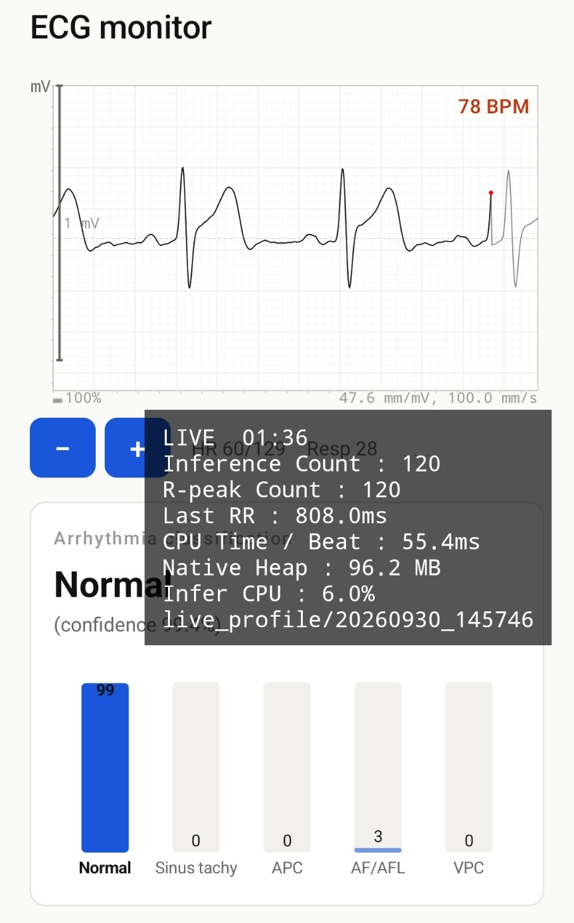
\includegraphics[width=\textwidth]{figures/live_profiler.png}
% \caption[Resource usage during live ECG streaming.]{Resource usage during live ECG streaming with the HiCardi patch:
% Monitor screen with the CPU and memory traces recorded on the target device.}
% \label{fig:live_profile}
% \end{figure}

% Fig.~\ref{fig:live_profile}은 측정 구간의 Monitor 화면과 CPU 및 메모리 사용량이다.
% 추론 스레드 CPU 사용률은 $7.9\%$, 수신 스레드는 $1.0\%$,
% 프로세스 전체 평균 CPU 사용률은 $46.3\%$였다.
% Peak Native Heap은 $99.2\,\mathrm{MB}$였다.

% 세션에서 $413$개의 beat가 기록되었으며,
% 측정 시간 $309.2056\,\mathrm{s}$를 기준으로 계산한 beat rate는
% $413/309.2056\times60=80.14\,\mathrm{bpm}$이다.
% 앱에서 보고된 평균 심박수는 $80.2\,\mathrm{bpm}$이다.
% $T_{\mathrm{beat}}$는 평균 $59.4\,\mathrm{ms}$,
% $P50$ $56.9\,\mathrm{ms}$, $P95$ $70.3\,\mathrm{ms}$로 측정되었다.
% $T_{\mathrm{queue}}$의 최댓값은 $11.4\,\mathrm{ms}$였다.
% 그리고 모두 Normal로 평가되었다.

% \begin{table}[t]
% \centering
% \caption[Resource usage during continuous ECG streaming.]{Resource usage during continuous ECG streaming with the HiCardi patch on Samsung SM-G996N (Exynos 2100).}
% \label{tab:live_profile}
% \small

% \begin{tabular}{@{}llr@{}}
% \toprule
% Group & Metric & Value \\
% \midrule
% \multirow{3}{*}{Session}
%  & Duration                        & 309.21\ s (approx. 5 min 9 s) \\
%  & Detected beats $N_{\mathrm{R}}$ & 413 \\
%  & Reported heart rate              & 80.2\ bpm \\
% \midrule
% \multirow{5}{*}{Processing}
%  & $T_{\mathrm{beat}}$ (Avg.)      & 59.4\ ms \\
%  & $T_{\mathrm{beat}}$ ($P5$)      & 49.7\ ms \\
%  & $T_{\mathrm{beat}}$ ($P50$)     & 56.9\ ms \\
%  & $T_{\mathrm{beat}}$ ($P95$)     & 70.3\ ms \\
%  & $T_{\mathrm{queue}}$ (max)      & 11.4\ ms \\
% \midrule
% \multirow{4}{*}{Resource}
%  & CPU, inference thread      & 7.9\ \% \\
%  & CPU, reception thread        & 1.0\ \% \\
%  & CPU, process                    & 46.3\ \% \\
%  & Peak Native Heap                        & 99.2\ MB \\
% \bottomrule
% \end{tabular}
% \end{table}


% \clearpage

% %%%%%%%%%%%%%%%%%%%%%%%%%%%%%%%%%%%%%%%%%%%%%%%%%%%%%
% % Chapter 6. Conclusion
% %%%%%%%%%%%%%%%%%%%%%%%%%%%%%%%%%%%%%%%%%%%%%%%%%%%%%
% \chapter{Conclusion} \label{ch:conclusion}

% 본 논문에서는 웨어러블 ECG 환경에서 실시간 부정맥 모니터링을 수행하기 위해 ResUMamba를 경량화하고 스마트폰 on-device 추론 시스템으로 구현하였다.
% 기존 ResUMamba는 ECG의 형태학적 특징을 추출하는 ResU path와 시간 의존성을 모델링하는 Mamba path를 결합한다. 본 연구에서는 Android CPU 배포를 위해 표준 ATen 연산 기반의 배포용 순차 scan을 사용하고, 모델 구조와 계산 표현을 함께 최적화하였다.

% 먼저 ResU path의 표준 1차원 합성곱을 depthwise separable convolution으로 대체한 ResDSUMamba를 구성하고 동일한 데이터 분할과 분류 목적 아래 재학습하였다.
% Mamba path는 학습된 ResDSUMamba의 가중치를 사용하고, selective scan의 계산을 PyTorch 표준 연산으로 표현한 순차 scan으로 ExecuTorch에 배포하였다.
% 실시간 실행을 위해 ECG 수신, 14-bit 샘플 복원, 원형 버퍼 관리, R-peak 위치 보정, 전처리 및 모델 추론으로 구성된 처리 과정을 구현하였다.
% 수신과 추론은 서로 다른 스레드에서 처리하였고, 통신 단절, 결측, 신호 포화 또는 전극 탈착이 감지되면 추론을 중지하였다가 유효한 ECG가 다시 확보된 이후 재개하도록 구성하였다.

% ResDSUMamba는 파라미터 수를 $2.488\,\mathrm{M}$에서 $1.323\,\mathrm{M}$으로
% $46.9\%$, MAC 수를 $721.50\,\mathrm{M}$에서 $331.38\,\mathrm{M}$으로
% $54.1\%$ 줄였다.
% HiCardi dataset의 record-wise split에서 ResUMamba의 Macro-$F_1$과 Micro-$F_1$은
% 각각 $42.28\%$와 $79.27\%$이고,
% ResDSUMamba는 각각 $44.15\%$와 $83.29\%$였다.
% Macro-Se는 각각 $78.00\%$와 $75.72\%$로 측정되었다.

% Galaxy~S21+에서 XNNPACK 구성의 평균 $T_{\mathrm{model}}$은
% ResUMamba $48.25\,\mathrm{ms}$, ResDSUMamba $36.70\,\mathrm{ms}$였다.
% DSConv 적용에 따른 두 모델의 평균 시간 차이는 $11.55\,\mathrm{ms}$,
% 상대 감소율은 $23.9\%$였다.
% ResDSUMamba의 $P95$는 $38.90\,\mathrm{ms}$로 측정되었다.

% 실제 HiCardi patch 스트리밍에서는 $309.21\,\mathrm{s}$ 동안
% $413$개의 beat가 처리되었으며, 앱에서 보고된 평균 심박수는 $80.2\,\mathrm{bpm}$였다.
% $T_{\mathrm{beat}}$는 평균 $59.4\,\mathrm{ms}$, $P95$ $70.3\,\mathrm{ms}$였고,
% 추론 스레드 CPU 사용률은 $7.9\%$, Peak Native Heap은 $99.2\,\mathrm{MB}$였다.
% 이 결과는 본 측정 조건에서 wearable patch ECG를 스마트폰에서 심박 단위로 처리하는
% on-device 스트리밍 파이프라인의 실행 결과를 보여준다.

% %% =================================================
% \section{Limitations and Future Work} \label{sec:conclusion_limitations}

% 본 연구의 실기기 평가는 Galaxy~S21+에서 309.21 s의 단일 세션으로 수행하였다. $T_{\mathrm{model}}$과 $T_{\mathrm{beat}}$을 측정하였으며, BLE 통신과 화면 표시를 포함한 end-to-end 지연, 전력 소비 및 장시간 동작에 따른 발열은 측정하지 않았다. 향후 연구에서는 다양한 심박수 조건과 장시간 측정, 복수의 모바일 단말을 대상으로 평가 범위를 확장한다.

% Live session에는 동기화된 ground-truth 임상 label이 포함되지 않았다. Live 환경에서는 처리시간과 자원 사용량을 측정하였으며, 향후 실제 부정맥 환자 의사판독과 배포된 모델과 비교할 예정이다.
% HiCardi 데이터셋은 환자 개인정보 보호를 위해 대중에 공개되지 않으나, 학술 및 연구 목적에 한하여 데이터 관리 주체의 정해진 승인 절차를 거쳐 접근할 수 있다.

% \clearpage


%%%%%%%%%%%%%%%%%%%%%%%%%%%%%%%%%%%%%%%%%%%%%%%%%%%%%
% Chapter 1. Introduction
%%%%%%%%%%%%%%%%%%%%%%%%%%%%%%%%%%%%%%%%%%%%%%%%%%%%%
\chapter{Introduction} \label{Ch:intro}


Cardiovascular disease (CVD) is one of the leading causes of death worldwide, making early diagnosis and continuous monitoring important.
Among cardiovascular disorders, arrhythmia, which arises from irregular electrical activity of the heart, can lead to serious complications such as hemodynamic instability, heart failure, and cardiac arrest.
Atrial fibrillation (AFIB), in particular, is a common form of arrhythmia and has been reported to increase the risk of stroke by approximately fivefold~\cite{wolf1991atrial}.
Paroxysmal arrhythmias are intermittent and often short-lived, so a standard 12-lead electrocardiogram (ECG) recorded for approximately $10\,\mathrm{s}$ may not capture every episode.
For this reason, long-term ECG monitoring with wearable patches has been used to detect intermittent arrhythmias~\cite{steinhubl2018wearable}.

Irregular pulse detection using smartwatches, followed by confirmatory ECG recording with an ECG patch, is another approach used for out-of-hospital arrhythmia detection~\cite{perez2019large}.
Continuous ECG monitoring with wearable patches has also been reported~\cite{steinhubl2018wearable}.
These devices can record cardiac activity with relatively little disruption to daily life, making them useful for long-term monitoring.
At the same time, reviewing the large amount of ECG data accumulated over several days or weeks is difficult to perform manually.
Automated ECG analysis is therefore needed to support long-term monitoring.

Early studies on automated ECG classification relied mainly on conventional signal-processing methods.
Typical approaches extracted delineation features such as beat intervals, QRS duration, and waveform amplitude, or manually designed morphological and temporal features and then used them as inputs to machine-learning classifiers~\cite{de2004automatic,melgani2008classification,luz2016ecg,raj2017ecg}.
Deep neural networks (DNNs) later became the dominant approach because they can learn feature extraction directly from the data in an end-to-end manner.
Representative models include convolutional neural networks (CNNs), which are effective at extracting local morphological patterns~\cite{niu2019inter,jing2021ecg}, recurrent neural networks (RNNs)~\cite{saadatnejad2019lstm,hou2019lstm} and state space models (SSMs)~\cite{lee2025atrial,bathini2026mamba}, which model temporal dependencies, and transformers~\cite{islam2024cat,che2021constrained}, which capture relationships across time steps.

Despite their high classification performance on known data, DNN models can degrade substantially when they are applied to previously unseen patients~\cite{llamedo2011heartbeat,jeong2024enhancing}.
ECG morphology depends not only on cardiac anatomy and physiological state but also on factors such as age, sex, underlying disease, electrode placement, and recording-device characteristics.
Consequently, a model may perform well in an intra-patient setting, where the same patient's beats appear in both training and evaluation data, but perform worse in an inter-patient setting, where the evaluation data contain patients not seen during training.

To address this variability, personalization methods that incorporate patient-specific baseline information into the model have been proposed~\cite{xu2019ivector, heo2026resumamba, fan2025class}.
Rather than relying only on absolute waveform morphology, personalization allows the model to focus on deviations from the patient's own baseline, which can reduce the effect of inter-patient morphological variation.
The main categories of personalization methods and the position of the target model are reviewed in Section~\ref{sec:bg_wearable}.

Most previous studies have focused on classification accuracy and personalization performance.
In comparison, relatively few studies have examined deep-learning models together with on-device streaming on mobile hardware and measurements obtained from an actual device.
A patient-conditioned architecture also introduces additional computation for extracting patient characteristics and combining them with classification features.
The original Mamba implementation provides a CUDA-accelerated selective-scan path as well as a pure PyTorch reference implementation~\cite{gu2023mamba}.
For mobile CPU deployment, this work uses a sequential scan implemented with standard ATen operators.

For wearable and mobile systems, it is not enough to classify isolated ECG segments; the system must continue processing beats as the ECG stream arrives.
In cloud-based analysis, raw ECG must be transmitted to a server, introducing an external communication path and computing dependency~\cite{park2024realtime}.
In contrast, on-device analysis performs ECG processing and inference directly on the target device.
In this work, real-time processing is defined as continuously constructing beat-level inputs from the incoming ECG stream and running classification inference for each beat.
Both model execution time and the processing time observed during actual streaming are measured.

The target model is patient-conditioned ResUMamba~\cite{heo2026resumamba}, which was proposed to improve inter-patient generalization.
This work adapts the model for beat-level execution on a smartphone through model lightweighting and deployment-oriented changes.
The convolutions in the ResU path are replaced with depthwise separable convolutions to reduce the model size and computational cost.
The selective scan in the Mamba path is rewritten into a form that can be executed using standard mobile CPU operators.
A smartphone application is also implemented to communicate with the HiCardi\textsuperscript{\textregistered} Smart Patch and to measure the complete streaming path from ECG reception to beat-level inference.
The experiments compare ResUMamba and ResDSUMamba using a record-wise split of the HiCardi\textsuperscript{\textregistered} dataset, and measure model execution time, streaming processing time, and resource usage on a Galaxy~S21+.

The contributions of this work are as follows.
\begin{itemize}
\item ResDSUMamba is constructed by replacing the standard convolutions in the ResU path of the existing ResUMamba with depthwise separable convolutions (DSConv) and replacing the decoder's transposed convolutions with parameter-free linear interpolation, followed by retraining on the HiCardi dataset.
\item The selective scan in the Mamba path is implemented as a sequential scan using standard PyTorch ATen operators and converted into a form that can run with ExecuTorch and the XNNPACK backend. Execution time is measured under different backend configurations.
\item A smartphone application is implemented to communicate with the HiCardi patch over BLE. Sample indices are used as the time axis, a circular buffer is used to construct beat segments, and ECG reception and inference are handled on separate threads.
\item The classification performance of ResUMamba and ResDSUMamba is compared on the HiCardi dataset, and model execution time, per-beat processing time during streaming, and resource usage are measured on an actual smartphone.
\end{itemize}


\clearpage

%%%%%%%%%%%%%%%%%%%%%%%%%%%%%%%%%%%%%%%%%%%%%%%%%%%%%
% Chapter 2. Background and Related Works
%%%%%%%%%%%%%%%%%%%%%%%%%%%%%%%%%%%%%%%%%%%%%%%%%%%%%
\chapter{Background and Related Works} \label{ch:background}

This chapter reviews the studies that form the basis of this work.
First, beat-level arrhythmia classification from wearable ECG and the problem of inter-patient variability are introduced, followed by the architecture of the patient-conditioned ResUMamba model.
Next, previous work on embedded and mobile arrhythmia classifiers is reviewed.
Finally, mobile DNN deployment frameworks and selective-scan implementations are discussed, with particular attention to the cost of parallel selective scan on a single-threaded CPU.

%% =================================================
\section{Inter-Patient Arrhythmia Classification from Wearable ECG} \label{sec:bg_wearable}

Approaches to inter-patient variability can be broadly divided into two groups.
The first is a generalization approach, which learns features that are shared across patients~\cite{de2004automatic,niu2019inter,jeong2024enhancing}.
The second is a personalization approach, which explicitly incorporates patient-specific information.

Among personalization methods, training a separate classifier for each patient~\cite{llamedo2012automatic,de2006patient,fan2025class} or fine-tuning a pretrained model with patient-specific data requires additional annotation and training for each new patient.
Such procedures can be difficult to apply in practical deployment.
An alternative is to extract an embedding that represents the patient and combine it with intermediate classification features.
For example, i-vector-based methods originally developed for speaker recognition have been adapted to ECG~\cite{xu2019ivector}.
Because a single model can then be shared across patients, this approach is more suitable for deployment.

Label-free patient conditioning~\cite{heo2026resumamba} takes this idea one step further by extracting a patient embedding from a baseline ECG without using arrhythmia labels.
The same model can then be used for a new patient without additional labeling or fine-tuning after deployment.
This makes the approach particularly attractive for wearable applications.
The ResUMamba model studied in this work follows this approach.

%% =================================================
\section{Patient-Conditioned ResUMamba} \label{sec:bg_resumamba}

% --------------------------------------------------------------------
\begin{figure}[t]
\centering
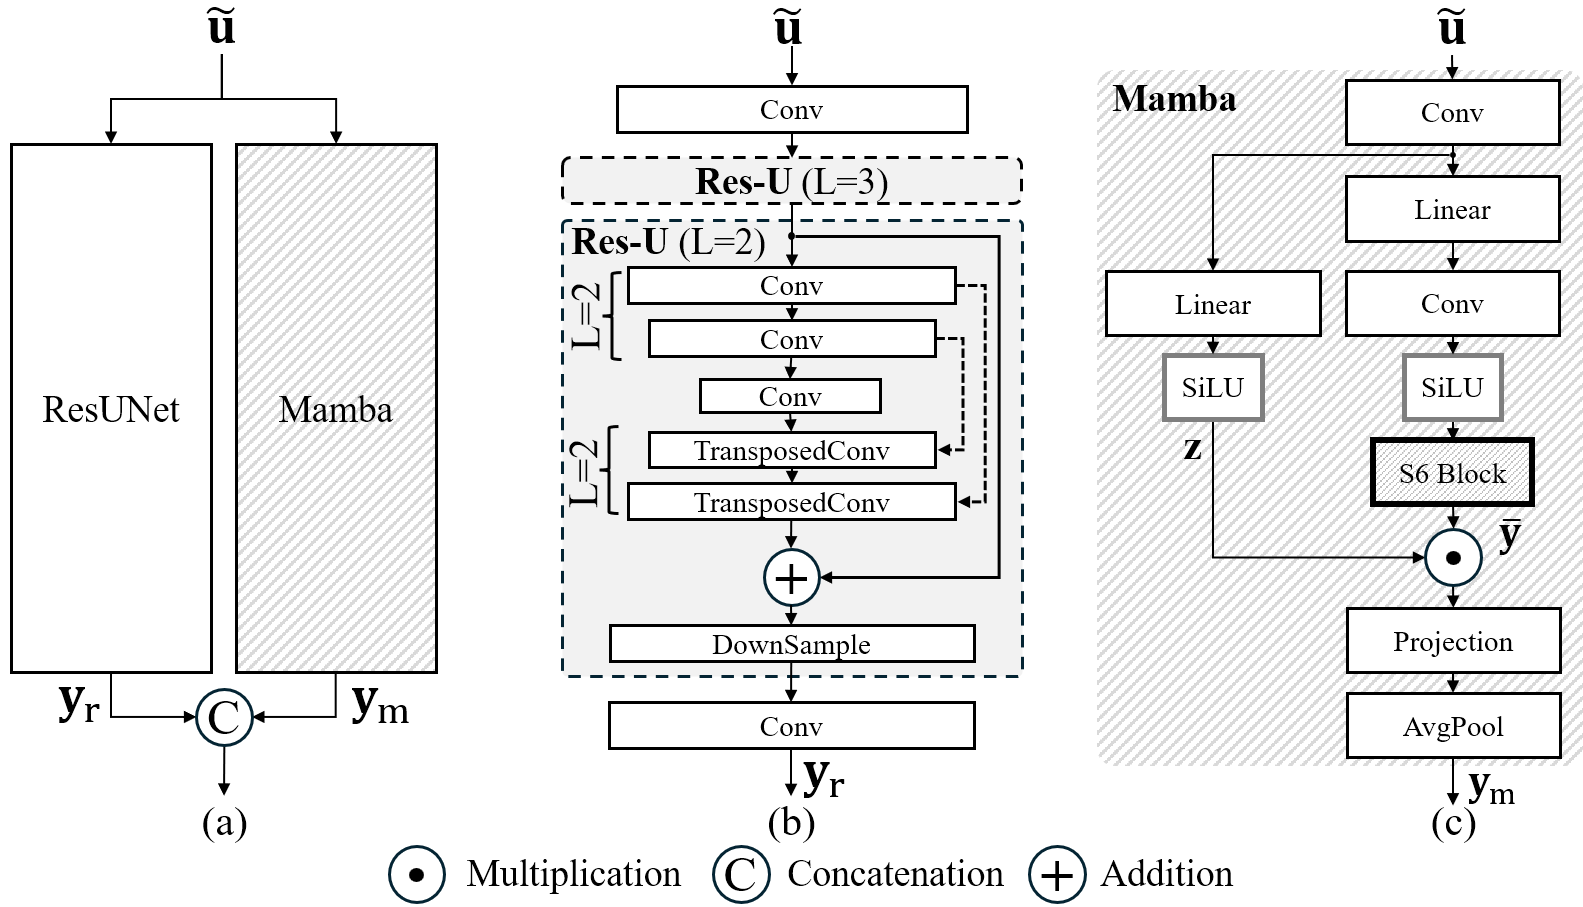
\includegraphics[width=\textwidth]{figures/ResUMamba.png}
\caption[Dual-path backbone of patient-conditioned ResUMamba~\cite{heo2026resumamba}.]{%
Dual-path backbone of patient-conditioned ResUMamba~\cite{heo2026resumamba}.
(a)~Parallel ResU and Mamba paths.
(b)~ResU path with two cascaded Res-U blocks.
(c)~Gated Mamba path with an S6 block.}
\label{fig:resumamba_arch}
\end{figure}
% --------------------------------------------------------------------

The target model of the real-time on-device implementation is the patient-conditioned ResUMamba model proposed for patient-conditioned beat classification~\cite{heo2026resumamba}. As shown in Fig.~\ref{fig:resumamba_arch}(a), the model uses a dual-path backbone in which an R-peak-aligned beat segment $\tilde{\mathbf{u}}$ is processed in parallel by the ResU and Mamba paths. The ResU path extracts morphological features from structures such as the P wave, QRS complex, and T wave using multiresolution convolutions, while the Mamba path models temporal dependencies within the beat using a selective state space model. The outputs of the two paths are concatenated and subsequently used for patient conditioning with a patient embedding vector (PEV) $\mathbf{p}$ obtained from the patient's baseline ECG. The conditioned representation is then combined with clinical features $\mathbf{c}$, such as RR intervals, before being passed to the classifier.

The ResU path is a residual U-Net~\cite{ronneberger2015unet,zhang2018resunet}-based architecture adapted for one-dimensional ECG.
As shown in Fig.~\ref{fig:resumamba_arch}(b), it consists of an input convolution, Res-U blocks with depths $L=3$ and $L=2$, and an output convolution.
Within each block, the temporal resolution is reduced through $L$ stride-2 convolutions, restored using transposed convolutions and skip connections, and then combined with the block input through a residual connection.
The resulting representation is downsampled before entering the next stage.
Because the path repeatedly uses standard one-dimensional convolutions, these operations account for a large part of the computational cost on a mobile device.

The Mamba path is based on a state space model (SSM).
An SSM discretizes a continuous-time linear system and updates its state with a computational cost that grows linearly with sequence length.
The Structured State Spaces for Sequence (S4) Family ~\cite{gu2021s4,gu2022parameterization} established the use of structured state-transition matrices, including diagonal parameterizations.
Mamba~\cite{gu2023mamba} introduced the selective state space model (S6), in which the discretization step and the input and output projections depend on the current input.
This allows the model to selectively retain information in its state.
As shown in Fig.~\ref{fig:resumamba_arch}(c), ResUMamba uses an input convolution followed by a gating branch (Linear--SiLU) and a main branch (Linear--Conv--SiLU--S6).
The outputs of the two branches are multiplied element-wise, then projected and average-pooled to obtain $\mathbf{y}_{m}$.
Let the input feature at time $t$ be $\mathbf{x}_t\in\mathbb{R}^{D}$ and the state be $\mathbf{H}_t\in\mathbb{R}^{D\times N}$.
The S6 update is given by

\begin{equation}
\begin{aligned}
\mathbf{H}_t &= \overline{\mathbf{A}}_t\odot\mathbf{H}_{t-1} + \mathbf{b}_t,
\qquad \mathbf{b}_t=(\boldsymbol{\delta}_t\odot\mathbf{x}_t)\mathbf{B}_t^{\top}, \\
\mathbf{y}_t &= \mathbf{H}_t\mathbf{C}_t + \mathbf{d}\odot\mathbf{x}_t.
\end{aligned}
\label{eq:selective_ssm}
\end{equation}

Here, $\boldsymbol{\delta}_t\in\mathbb{R}^{D}$ denotes the discretization step, and $\mathbf{B}_t,\mathbf{C}_t\in\mathbb{R}^{N}$ are the vectors that write the input into the state and read the state into the output, respectively.
All three are generated from $\mathbf{x}_t$.
$\mathbf{A}\in\mathbb{R}^{D\times N}$ contains the channel-wise diagonal state-transition parameters.
Accordingly, the discretized transition is defined as
$\overline{\mathbf{A}}_t=\exp(\boldsymbol{\delta}_t\mathbf{1}_N^{\top}\odot\mathbf{A})$,
where $\mathbf{d}\in\mathbb{R}^{D}$ is the skip coefficient.
The operator $\odot$ denotes element-wise multiplication, and the computational cost for a sequence of length $T$ is $\mathcal{O}(TDN)$.
Because $\mathbf{H}_t$ depends on $\mathbf{H}_{t-1}$, directly evaluating Eq.~\eqref{eq:selective_ssm} requires $T$ sequential update steps.


The PEV $\mathbf{p}$ provides the patient-conditioning information used
by the classifier.
It is obtained from a short, label-free calibration ECG segment using
an encoder trained with contrastive predictive coding (CPC)-based
self-supervised learning~\cite{oord2018cpc}.
The encoder maps the calibration segment to a fixed-dimensional
representation that summarizes patient-specific ECG characteristics.
Because the calibration procedure does not require arrhythmia labels,
the same procedure can be applied to a new patient without additional
labeling or model fine-tuning.



%% =================================================
\section{On-Device ECG Classification and Mobile Deployment}
\label{sec:bg_mobile_deployment}

Real-time arrhythmia classification for wearable and mobile devices has
been investigated using CNN-, RNN-, and TCN-based models, including
implementations on wearable platforms and microcontrollers
~\cite{kiranyaz2016realtime,faraone2020crnn,ingolfsson2021ecgtcn,lee2022compressed}.
More recently, state-space model (SSM)-based approaches have also been
explored for ECG analysis~\cite{lee2025atrial,bathini2026mamba}, and
inter-patient arrhythmia classifiers have been investigated for
edge-oriented deployment~\cite{xu2026cardiolike}.
A real-time ECG service based on HiCardi uses a smartphone for data
transfer and user interaction, while signal analysis is performed on a
server~\cite{park2024realtime}. In contrast, the present work targets
on-device execution of the patient-conditioned ResUMamba model,
including the complete streaming path from BLE reception and buffering
to R-peak alignment and beat-level inference.

On-device execution requires a model representation and runtime that
are supported by the target mobile platform.
TensorFlow Lite~\cite{tflite}, ExecuTorch~\cite{executorch}, and ONNX
Runtime~\cite{onnxruntime} provide mobile or edge execution frameworks
for trained neural networks. In the PyTorch ecosystem, ExecuTorch uses
\texttt{torch.export} to obtain an exportable computational graph and
supports delegation of supported subgraphs to optimized backend
implementations. XNNPACK~\cite{xnnpack} provides optimized kernels for
mobile CPU execution, including common operations such as convolution
and linear algebra, and can be used as a backend in both TensorFlow
Lite and ExecuTorch. In ExecuTorch, operations supported by XNNPACK are
executed through the delegated backend, whereas unsupported operations
remain on the portable-kernel path. This distinction is important
because the practical latency of a model depends not only on its
parameter count or theoretical computational cost, but also on how its
operators are supported by the target runtime and hardware.

This consideration is particularly important for SSM-based models.
The official Mamba implementation provides a CUDA-accelerated
selective-scan implementation together with a reference PyTorch path
~\cite{gu2023mamba}. The CUDA extension is not available on the Android
CPU target considered in this work. Therefore, the selective SSM
recurrence in Eq.~\eqref{eq:selective_ssm} is expressed using standard
ATen operators so that it can be represented in the exported graph and
executed on the mobile CPU. Although parallel prefix-scan algorithms
can reduce sequential depth on parallel hardware
~\cite{hillis1986data,blelloch1990prefix,harris2007parallel}, they were
not adopted here because the target deployment uses a single CPU
execution thread and the study focuses on a standard operator graph
rather than a dedicated scan implementation.

Model-level lightweighting techniques such as depthwise separable
convolution, quantization, pruning, and knowledge distillation can
reduce computational cost~\cite{howard2017mobilenets,jacob2018quantization,
hinton2015distilling}. However, a reduction in theoretical computation
does not necessarily translate into lower latency when the resulting
operators are not efficiently supported by the target runtime.
Related SSM deployment studies have therefore explored specialized
operator implementations or dedicated hardware, such as MCU-oriented
MambaLite-Micro~\cite{xu2025mambalite} and NPU-oriented XAMBA
~\cite{das2025xamba}. Unlike these approaches, the present work focuses
on smartphone CPU execution using standard ExecuTorch operators and
XNNPACK delegation, with model lightweighting and runtime support
considered together for practical on-device ECG inference.
 
\clearpage



%%%%%%%%%%%%%%%%%%%%%%%%%%%%%%%%%%%%%%%%%%%%%%%%%%%%%
% Chapter 3. Model Optimization and Deployment
%%%%%%%%%%%%%%%%%%%%%%%%%%%%%%%%%%%%%%%%%%%%%%%%%%%%%

\chapter{Model Optimization and Deployment for On-Device Inference}
\label{ch:optimization}

This chapter describes the model-level optimization and deployment methods used to execute ResUMamba in real time on a smartphone.
The overall system architecture is shown in Fig.~\ref{fig:overall_architecture}.
Section~\ref{sec:opt_targets} defines the optimization objectives and constraints, and Section~\ref{sec:opt_resu} applies depthwise separable convolution to the ResU path.
Section~\ref{sec:opt_mamba} rewrites the selective scan in the Mamba path as a sequential scan executable on the mobile runtime.
The patient-conditioning mechanism, clinical-feature fusion, model input and output, and training procedure remain unchanged.
\begin{figure*}[t]
\centering
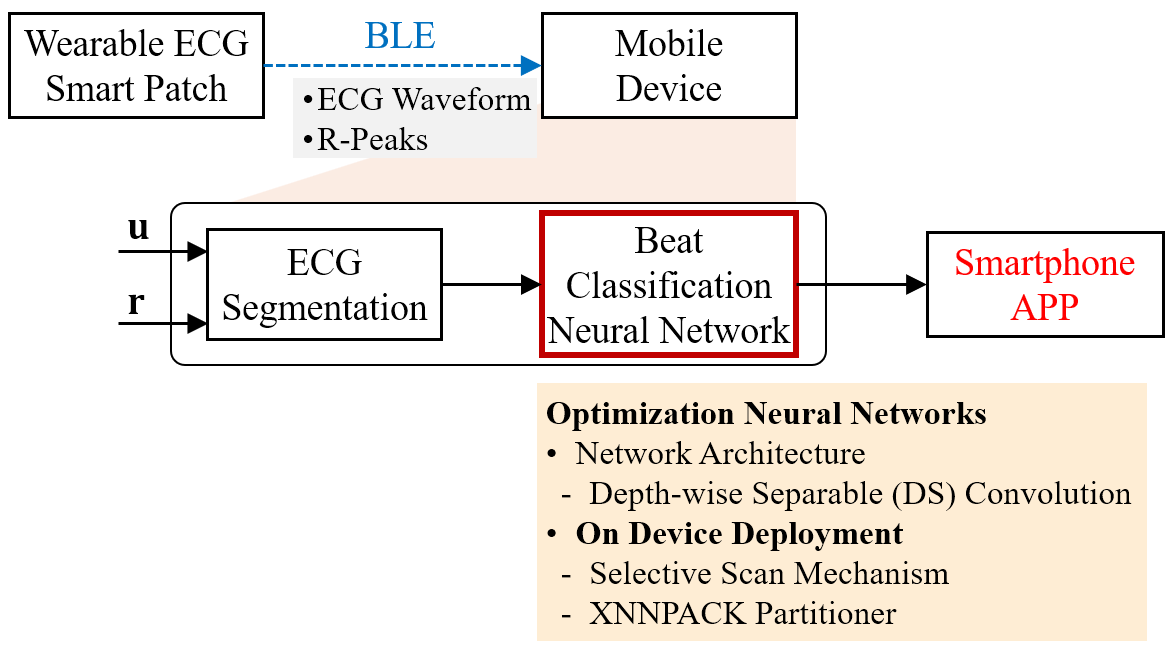
\includegraphics[width=0.95\textwidth]{figures/Overall Architecture.png}
\caption{Overall system architecture from wearable ECG acquisition to optimized on-device inference.}
\label{fig:overall_architecture}
\end{figure*}

%% =================================================
\section{Optimization Targets and Constraints} \label{sec:opt_targets}
The goal of this work is to run ResUMamba on a smartphone connected to a wearable patch and process the ECG on a beat-by-beat basis.
To support this deployment, the number of parameters and MACs is reduced, and CPU execution time is measured on the target device.

The CPU execution time of a single forward pass with a prepared beat input is denoted by $T_{\mathrm{model}}$ and is used as the main model-level timing metric.
In a streaming setting, however, model execution is only part of the total processing path.
Each beat must be processed before subsequent inputs accumulate.
We therefore report the mean, $P5$, $P50$, and $P95$ of $T_{\mathrm{model}}$ and additionally measure $T_{\mathrm{beat}}$ and $T_{\mathrm{queue}}$ during live streaming.
The R-peak detector uses a minimum interval of $240\,\mathrm{ms}$ between consecutive R-peaks.

The ResU path repeatedly applies standard convolutions and therefore accounts for a substantial portion of the model's computational cost.
These convolutions are replaced with depthwise separable convolutions to reduce both computation and parameter count.
The resulting ResDSUMamba model is retrained using the same HiCardi classification setting.
The Mamba path then uses the weights of the retrained ResDSUMamba, and its computational representation is converted to an ATen-based sequential scan during export.
Pruning was also evaluated as an alternative lightweighting method and was found unsuitable for this deployment target; the corresponding experiments and the rationale for instead adopting DSConv are reported in Appendix~\ref{app:pruning}.

%% ==================================================================
\section{ResU Path: Depthwise Separable Convolution}
\label{sec:opt_resu}
 
% --------------------------------------------------------------------
\begin{figure}[t]
\centering
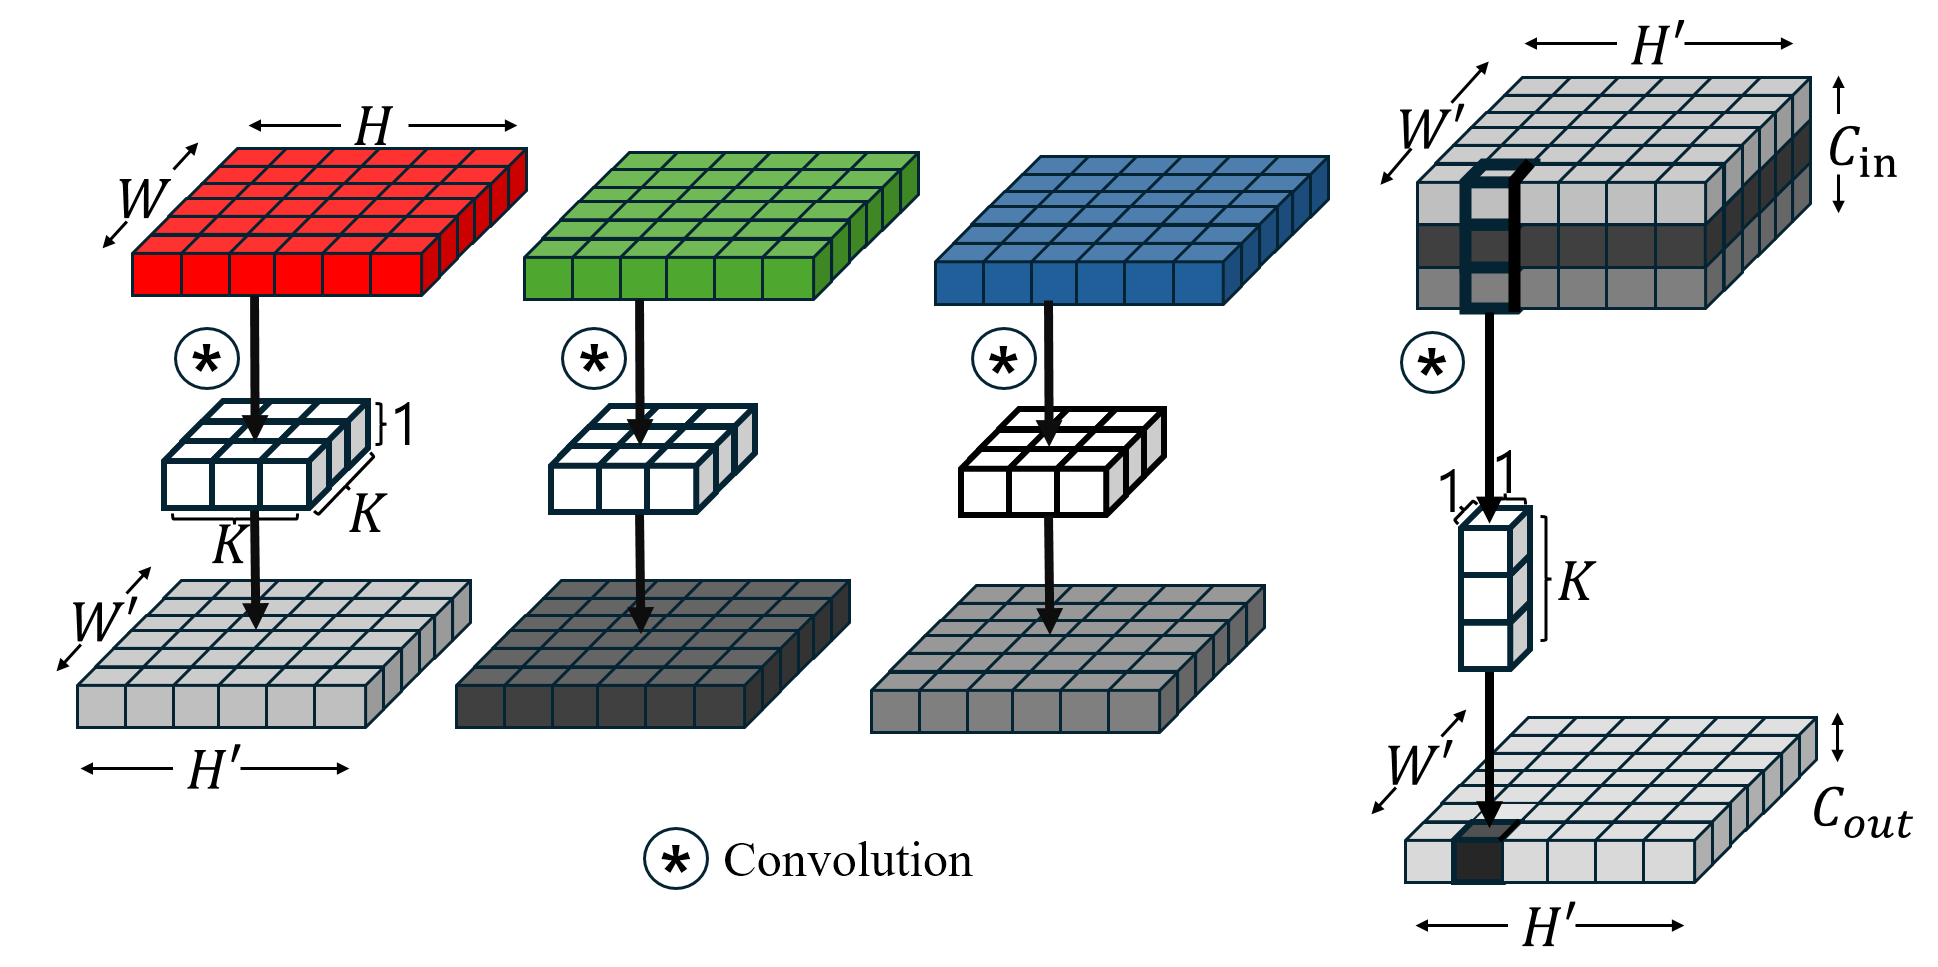
\includegraphics[width=\textwidth]{figures/dsconv.png}
\caption[Depthwise separable convolution~\cite{howard2017mobilenets}.]{%
Depthwise separable convolution: independent channel-wise filtering followed by $1\times1$ pointwise convolution for channel mixing.}
\label{fig:dsconv}
\end{figure}
% --------------------------------------------------------------------
 
Depthwise separable convolution (DSConv)~\cite{howard2017mobilenets} separates the temporal filtering and channel mixing performed jointly by a standard convolution into two stages.
MobileNets adopted this structure as a core building block for mobile vision models and helped popularize lightweight convolutional architectures.
As shown in Fig.~\ref{fig:dsconv}, DSConv consists of a depthwise convolution that applies an independent filter to each input channel and a pointwise convolution with kernel size $1$ that mixes information across channels.
Let the input and output channel vectors at time $t$ be $\mathbf{x}_t\in\mathbb{R}^{C_{\mathrm{in}}}$ and $\mathbf{y}_t\in\mathbb{R}^{C_{\mathrm{out}}}$, respectively.
A standard one-dimensional convolution with kernel size $K$ is defined as
\begin{equation}
\mathbf{y}_t = \sum_{j=0}^{K-1} \mathbf{W}_j\mathbf{x}_{t-j},\qquad
\mathbf{W}_j\in\mathbb{R}^{C_{\mathrm{out}}\times C_{\mathrm{in}}},
\label{eq:standard_conv1d}
\end{equation}
where stride and padding are omitted for clarity.
At each time step, a matrix-vector product of size $C_{\mathrm{out}}\times C_{\mathrm{in}}$ is performed $K$ times.
Thus, excluding bias terms, the number of parameters $P_{\mathrm{conv}}$ and multiply-accumulate (MAC) operations $M_{\mathrm{conv}}$ for an output length $\tilde{T}$ are
\begin{equation}
P_{\mathrm{conv}} = K C_{\mathrm{in}} C_{\mathrm{out}},\qquad
M_{\mathrm{conv}} = \tilde{T} K C_{\mathrm{in}} C_{\mathrm{out}}.
\label{eq:conv_complexity}
\end{equation}
DSConv first applies an independent $K$-tap temporal filter to each input channel:
\begin{equation}
\mathbf{z}_t = \sum_{j=0}^{K-1} \mathbf{g}_j \odot \mathbf{x}_{t-j},\qquad
\mathbf{g}_j \in \mathbb{R}^{C_{\mathrm{in}}},
\label{eq:depthwise_conv1d}
\end{equation}
where $\odot$ denotes channel-wise multiplication and no channel mixing is performed.
A pointwise convolution then combines channel information at the same time step using a matrix $\mathbf{Q}$:
\begin{equation}
\mathbf{y}_t = \mathbf{Q}\mathbf{z}_t,\qquad
\mathbf{Q}\in\mathbb{R}^{C_{\mathrm{out}}\times C_{\mathrm{in}}}.
\label{eq:pointwise_conv1d}
\end{equation}
Therefore, the number of parameters and MAC operations for DSConv are
\begin{equation}
P_{\mathrm{DS}} = K C_{\mathrm{in}} + C_{\mathrm{in}}C_{\mathrm{out}},\qquad
M_{\mathrm{DS}} = \tilde{T} \left(K C_{\mathrm{in}} + C_{\mathrm{in}}C_{\mathrm{out}} \right).
\label{eq:dsconv_complexity}
\end{equation}
 
% --------------------------------------------------------------------
\begin{figure}[t]
\centering
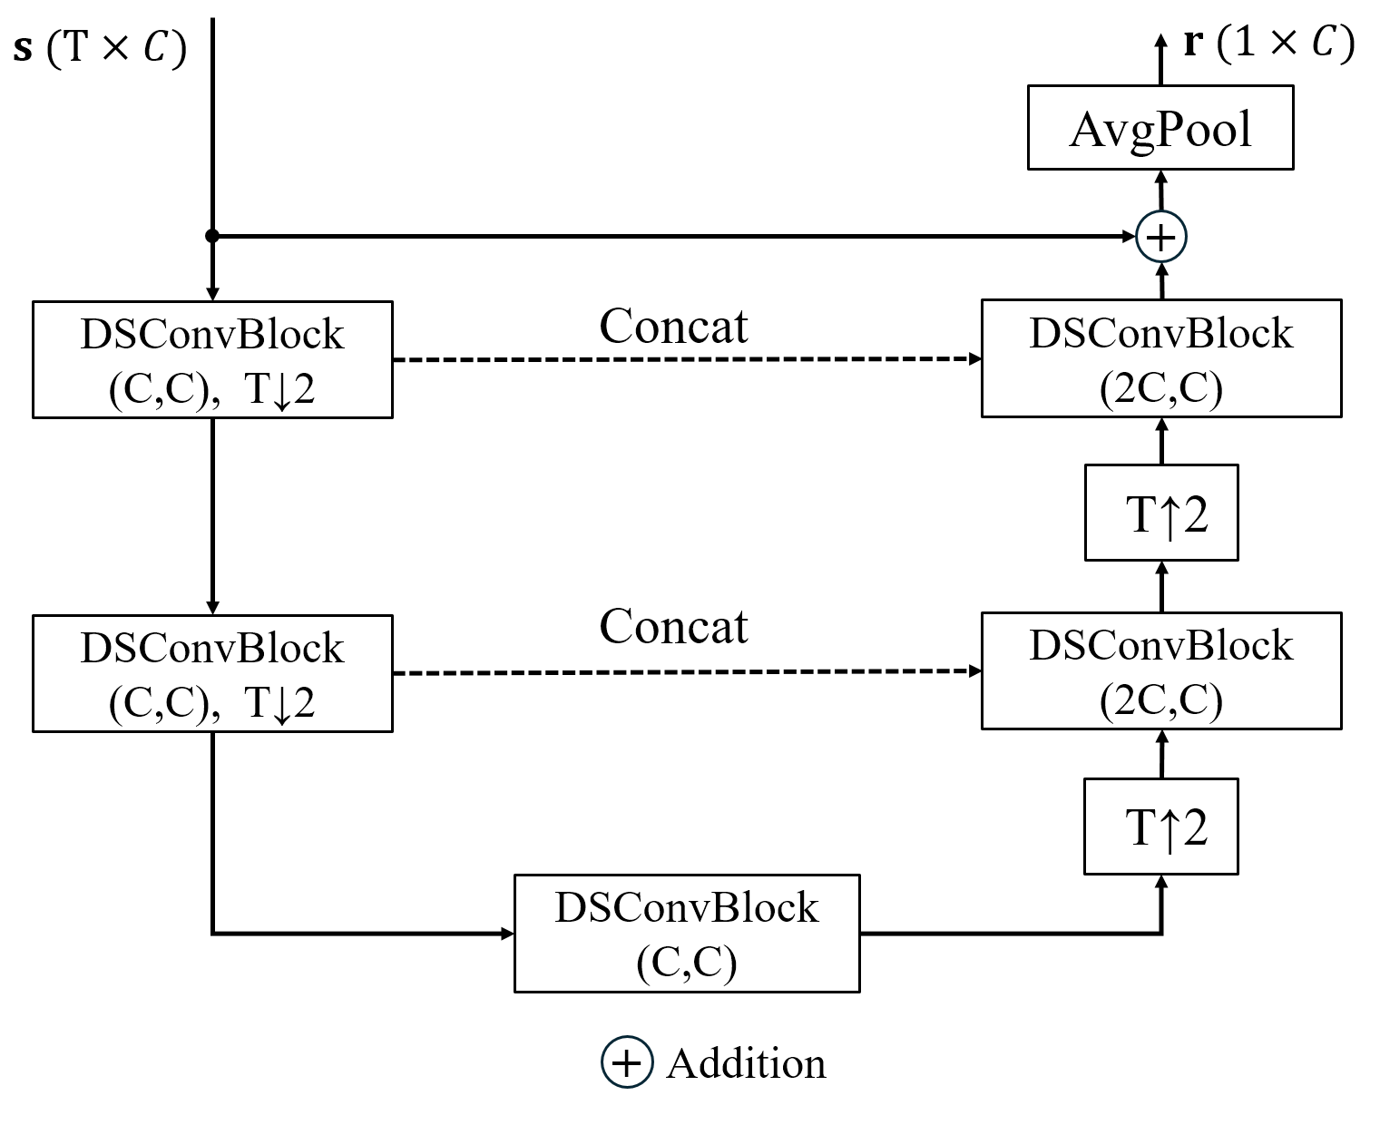
\includegraphics[width=0.9\textwidth]{figures/ResDSUNet.png}
\caption[Single Res-U block ($L=2$).]{%
A single Res-U block with encoder--decoder layer depth $L=2$, skip connections, residual addition, and average pooling to produce $\mathbf{y}_{r}$. The ResU path cascades two such blocks with depths $L=3$ and $L=2$ (Section~\ref{sec:bg_resumamba}).
T$\uparrow$2: parameter-free linear interpolation.}
\label{fig:resu_path}
\end{figure}
% --------------------------------------------------------------------
 
The relative computational cost of DSConv compared with a standard convolution is
$M_{\mathrm{DS}}/M_{\mathrm{conv}} = 1/C_{\mathrm{out}} + 1/K$.
For example, with $K=7$ and $C_{\mathrm{out}}=128$, a standard convolution needs $7\cdot128=896$ MACs per input channel and output step, whereas DSConv needs $7+128=135$, which is $15.1\%$ of the original, a reduction of $1-(1/128+1/7)\approx84.9\%$.
In this work, the convolutions of the encoder blocks, bottleneck block, and decoder blocks of the ResU path in Fig.~\ref{fig:resu_path} are replaced with DSConv, and these convolutions use $K=7$ and $C_{\mathrm{out}}=128$.
In the implementation used in this work, the decoder restores the temporal length with parameter-free linear interpolation (T$\uparrow$2 in Fig.~\ref{fig:resu_path}) instead of the transposed convolutions of the original model, and the decoder convolutions that follow the skip concatenation are replaced with DSConv.
 
Table~\ref{tab:params_macs} summarizes the parameter counts and module-wise MACs of the two models for an input length of $501$.
MACs include only multiply-accumulate operations in convolutions, linear layers, matrix multiplications, including batched matrix multiplications, and attention.
Element-wise operations, including normalization, activation functions, and the element-wise state update in the scan,
$\overline{\mathbf{A}}_t\odot\mathbf{H}_{t-1}+\mathbf{b}_t$,
are excluded.
The MAC count of the ResU path decreases from $490.27\,\mathrm{M}$ to $100.15\,\mathrm{M}$, a reduction of $79.6\%$, which is smaller than the layer-level value of $84.9\%$.
Because the ratio $1/C_{\mathrm{out}}+1/K$ does not depend on $C_{\mathrm{in}}$, the decoder convolutions that receive the $2C$-channel concatenation reach the same layer-level reduction as the other replaced convolutions.
The gap therefore comes from the operations that are not replaced: the downsampling layers between Res-U blocks and the kernel-size-$1$ residual shortcut convolutions, which cannot be factorized further.
Their MACs are the same in both models, so they make up a larger share of the reduced total.
The replacement of the decoder's transposed convolutions with parameter-free linear interpolation removes additional MACs beyond the per-layer DSConv substitution, but this interpolation cost is small relative to the convolutional layers, so the unreplaced downsampling and shortcut convolutions remain the dominant contributor to the gap between the measured $79.6\%$ reduction and the $84.9\%$ layer-level value.
The Mamba path, patient conditioning, feature fusion, and classifier are unchanged.
Consequently, the total MAC count of the model decreases by $54.1\%$ ($721.50\,\mathrm{M}\rightarrow331.38\,\mathrm{M}$), and the parameter count decreases by $46.9\%$ ($2.4883\,\mathrm{M}\rightarrow1.3225\,\mathrm{M}$).
 
\begin{table}[t]
\centering
\caption[Parameters and module-wise MACs.]{Parameters and module-wise MACs (input length $501$, batch $1$).
Element-wise operations, including the scan state update, are excluded.
The cross-attention row counts only the attention-weight matrix multiplications ($\mathbf{QK}^\top$ and the attention-weighted sum), which have no associated trainable parameters and are therefore omitted from the parameter rows.}
\label{tab:params_macs}
\small
\begin{tabular}{@{}lrrr@{}}
\toprule
Module & ResUMamba & ResDSUMamba & $\Delta$ \\
\midrule
\multicolumn{4}{@{}l}{MACs (M)} \\
\quad Input convolution & 0.07 & 0.07 & -- \\
\quad ResU path & 490.27 & 100.15 & $-79.6\%$ \\
\quad Mamba path & 129.28 & 129.28 & -- \\
\quad Patient conditioning & 0.26 & 0.26 & -- \\
\quad Fusion, classifier & 98.78 & 98.78 & -- \\
\quad Cross-attention & 2.84 & 2.84 & -- \\
\quad Total & 721.50 & 331.38 & $-54.1\%$ \\
\midrule
\multicolumn{4}{@{}l}{Parameters (M)} \\
\quad Input convolution & 0.0004 & 0.0004 & -- \\
\quad ResU path & 1.4787 & 0.3128 & $-78.8\%$ \\
\quad Mamba path & 0.2653 & 0.2653 & -- \\
\quad Patient conditioning & 0.2632 & 0.2632 & -- \\
\quad Fusion, classifier & 0.4807 & 0.4807 & -- \\
\quad Total & 2.4883 & 1.3225 & $-46.9\%$ \\
\bottomrule
\end{tabular}
\end{table}
 
Depthwise convolution performs relatively many memory accesses compared with its arithmetic workload and therefore has low arithmetic intensity.
Consequently, the reduction in theoretical operation count does not necessarily translate directly into an equivalent reduction in actual execution time.
In addition, depthwise and pointwise convolutions have different data layouts and tiling characteristics, making fusion into a single kernel difficult in general-purpose CPU libraries.
An intermediate tensor must therefore be materialized between the two stages.
The excluded element-wise scan update also remains unchanged by DSConv.
The resulting change in execution time on the target device is evaluated in Section~\ref{sec:exp_backend}.

%% =================================================
\section{Mamba Path: Rewriting the Selective Scan for Mobile Deployment}
\label{sec:opt_mamba}
 
Mamba provides an official CUDA-accelerated selective-scan path, but the selective SSM itself can be represented using standard tensor operations~\cite{gu2023mamba}.
Because CUDA extensions cannot be used for Android CPU deployment, this work uses a deployment-oriented sequential scan that constructs the recurrence in Eq.~\eqref{eq:selective_ssm} from standard PyTorch ATen operators.
DSConv is applied during training, whereas the selective scan is transformed during export.
The export stage uses the trained weights and converts the computational representation into ATen operations.
This implementation is referred to below as the deployment-oriented sequential scan.
 
% --------------------------------------------------------------------
\begin{figure}[t]
\centering
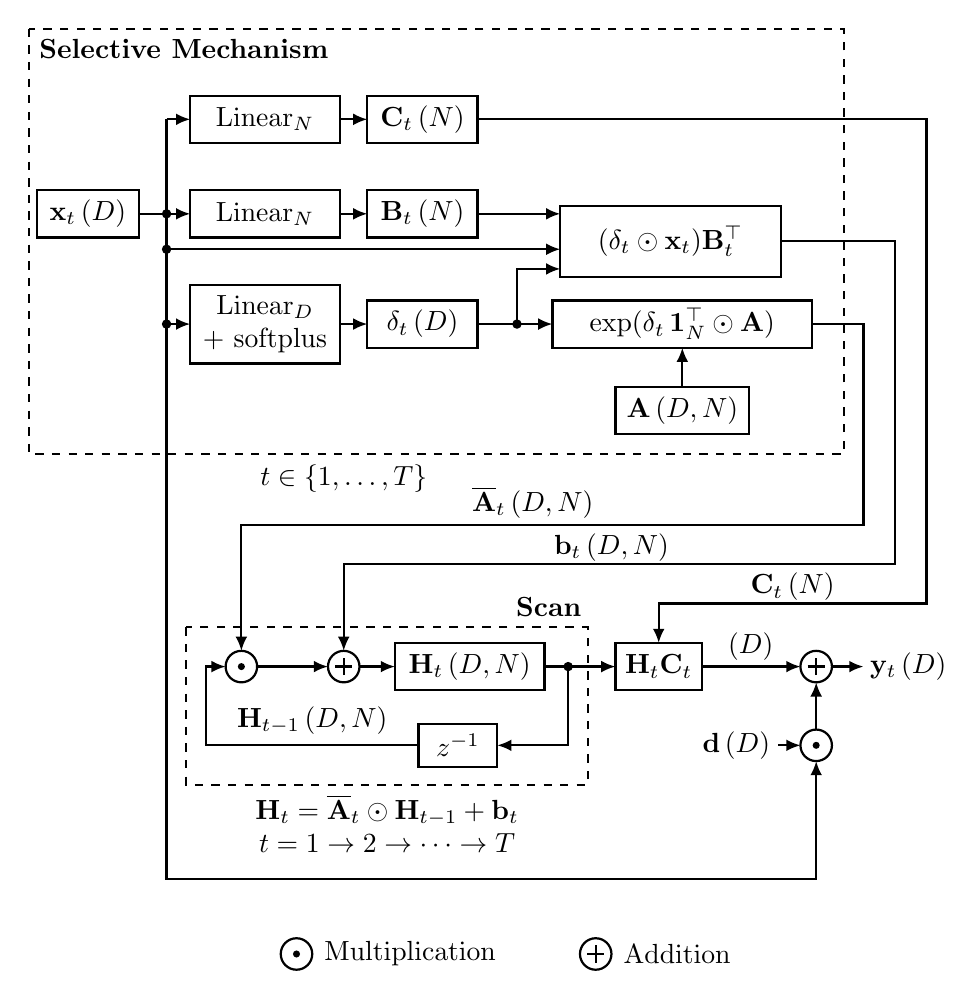
\begin{tikzpicture}[
    font=\normalsize,
    line width=0.8pt,
    arr/.style={-{Latex[length=1.8mm,width=1.5mm]}},
    blk/.style={draw,inner sep=1pt,align=center,minimum height=0.60cm},
    grp/.style={draw,dashed},
  ]
  % ---------------- Selective SSM (per-step computations) ----------------
  \draw[grp] (0.000,0.350) rectangle (10.350,-5.050);
  \node[anchor=north west,inner sep=2pt,align=left] at (0.050,0.300) {\textbf{Selective Mechanism}};
  \node[anchor=north,inner sep=2pt,align=center] at (4.000,-5.100) {$t\in\{1,\dots,T\}$};

  \node[blk,minimum width=1.30cm] at (0.750,-2.000) {$\mathbf{x}_{t}\,(D)$};
  \draw (1.400,-2.000) -- (1.750,-2.000);
  \draw (1.750,-0.800) -- (1.750,-3.400);
  \fill (1.750,-2.000) circle (0.06);
  \fill (1.750,-2.450) circle (0.06);
  \fill (1.750,-3.400) circle (0.06);
  \draw[arr] (1.750,-0.800) -- (2.050,-0.800);
  \draw[arr] (1.750,-2.000) -- (2.050,-2.000);
  \draw[arr] (1.750,-3.400) -- (2.050,-3.400);

  \node[blk,minimum width=1.90cm] at (3.000,-0.800) {Linear$_{N}$};
  \node[blk,minimum width=1.90cm] at (3.000,-2.000) {Linear$_{N}$};
  \node[blk,minimum width=1.90cm,minimum height=1.00cm] at (3.000,-3.400) {Linear$_{D}$\\+ softplus};
  \draw[arr] (3.950,-0.800) -- (4.300,-0.800);
  \draw[arr] (3.950,-2.000) -- (4.300,-2.000);
  \draw[arr] (3.950,-3.400) -- (4.300,-3.400);

  \node[blk,minimum width=1.40cm] at (5.000,-0.800) {$\mathbf{C}_{t}\,(N)$};
  \node[blk,minimum width=1.40cm] at (5.000,-2.000) {$\mathbf{B}_{t}\,(N)$};
  \node[blk,minimum width=1.40cm] at (5.000,-3.400) {$\boldsymbol{\delta}_{t}\,(D)$};

  \draw[arr] (5.700,-2.000) -- (6.750,-2.000);
  \draw[arr] (1.750,-2.450) -- (6.750,-2.450);
  \draw[arr] (5.700,-3.400) -- (6.650,-3.400);
  \fill (6.200,-3.400) circle (0.06);
  \draw[arr] (6.200,-3.400) -- (6.200,-2.700) -- (6.750,-2.700);

  \node[blk,minimum width=2.80cm,minimum height=0.90cm] at (8.150,-2.350) {$(\boldsymbol{\delta}_{t}\odot\mathbf{x}_{t})\mathbf{B}_{t}^{\top}$};
  \node[blk,minimum width=3.30cm] at (8.300,-3.400) {$\exp(\boldsymbol{\delta}_{t}\,\mathbf{1}_{N}^{\top}\odot\mathbf{A})$};
  \node[blk,minimum width=1.70cm] at (8.300,-4.500) {$\mathbf{A}\,(D,N)$};
  \draw[arr] (8.300,-4.200) -- (8.300,-3.700);

  % ---------------- outputs of the per-step part ----------------
  \draw[arr] (5.700,-0.800) -- (11.400,-0.800) -- (11.400,-6.950) -- (8.000,-6.950) -- (8.000,-7.450);
  \draw[arr] (9.550,-2.350) -- (11.000,-2.350) -- (11.000,-6.450) -- (4.000,-6.450) -- (4.000,-7.550);
  \draw[arr] (9.950,-3.400) -- (10.600,-3.400) -- (10.600,-5.950) -- (2.700,-5.950) -- (2.700,-7.550);
  \node[anchor=south,inner sep=2pt,align=center] at (6.400,-5.950) {$\overline{\mathbf{A}}_{t}\,(D,N)$};
  \node[anchor=south,inner sep=2pt,align=center] at (7.400,-6.500) {$\mathbf{b}_{t}\,(D,N)$};
  \node[anchor=south,inner sep=2pt,align=center] at (9.700,-7.00) {$\mathbf{C}_{t}\,(N)$};

  % ---------------- sequential scan ----------------
  \draw[grp] (2.000,-7.250) rectangle (7.100,-9.250);
  \node[anchor=south east,inner sep=2pt,align=right] at (7.100,-7.200) {\textbf{Scan}};
  \node[anchor=north,inner sep=2pt,align=center] at (4.550,-9.300) {$\mathbf{H}_{t}=\overline{\mathbf{A}}_{t}\odot\mathbf{H}_{t-1}+\mathbf{b}_{t}$\\$t=1\to2\to\cdots\to T$};

  % element-wise product: circle with a single dot (ISPLAB convention)
  \draw[fill=white] (2.700,-7.750) circle (0.2); \fill (2.700,-7.750) circle (0.045);
  % addition
  \draw[fill=white] (4.000,-7.750) circle (0.2); \draw (3.890,-7.750) -- (4.110,-7.750) (4.000,-7.860) -- (4.000,-7.640);
  \draw[arr] (2.900,-7.750) -- (3.800,-7.750);

  \node[blk,minimum width=1.90cm] at (5.600,-7.750) {$\mathbf{H}_{t}\,(D,N)$};
  \draw[arr] (4.200,-7.750) -- (4.650,-7.750);
  \fill (6.850,-7.750) circle (0.06);
  \draw[arr] (6.550,-7.750) -- (7.450,-7.750);
  \node[blk,minimum width=1.10cm] at (8.000,-7.750) {$\mathbf{H}_{t}\mathbf{C}_{t}$};

  \draw[arr] (6.850,-7.750) -- (6.850,-8.750) -- (5.950,-8.750);
  \node[blk,minimum width=1.00cm,minimum height=0.55cm] at (5.450,-8.750) {$z^{-1}$};
  \draw[arr] (4.950,-8.750) -- (2.250,-8.750) -- (2.250,-7.750) -- (2.500,-7.750);
  \node[anchor=south,inner sep=2pt,align=center] at (3.600,-8.700) {$\mathbf{H}_{t-1}\,(D,N)$};

  % ---------------- readout and skip ----------------
  \draw[arr] (8.550,-7.750) -- (9.800,-7.750);
  \node[anchor=south,inner sep=2pt,align=center] at (9.170,-7.750) {$(D)$};
  \draw[fill=white] (10.000,-7.750) circle (0.2); \draw (9.890,-7.750) -- (10.110,-7.750) (10.000,-7.860) -- (10.000,-7.640);
  \draw[arr] (10.200,-7.750) -- (10.600,-7.750);
  \node[anchor=west,inner sep=2pt,align=left] at (10.600,-7.750) {$\mathbf{y}_{t}\,(D)$};

  \draw[fill=white] (10.000,-8.750) circle (0.2); \fill (10.000,-8.750) circle (0.045);
  \draw[arr] (10.000,-8.550) -- (10.000,-7.950);
  \node[anchor=east,inner sep=2pt,align=right] at (9.500,-8.750) {$\mathbf{d}\,(D)$};
  \draw[arr] (9.520,-8.750) -- (9.800,-8.750);
  \draw[arr] (1.750,-3.400) -- (1.750,-10.450) -- (10.000,-10.450) -- (10.000,-8.950);
  

  % ---------------- Legend ----------------
  \draw[fill=white] (3.400,-11.400) circle (0.2); \fill (3.400,-11.400) circle (0.045);
  \node[anchor=west,inner sep=4pt] at (3.600,-11.400) {Multiplication}; % 이 부분 수정

  \draw[fill=white] (7.200,-11.400) circle (0.2); \draw (7.090,-11.400) -- (7.310,-11.400) (7.200,-11.510) -- (7.200,-11.290);
  \node[anchor=west,inner sep=4pt] at (7.400,-11.400) {Addition};

\end{tikzpicture}
\caption[Selective SSM (S6) of the Mamba path.]{%
Selective SSM (S6) of the Mamba path.
All terms except the state update are computed independently at each step;
only the state update is sequential.
$z^{-1}$: one-step delay.}
\label{fig:ssm_block}
\end{figure}
% --------------------------------------------------------------------
 
Fig.~\ref{fig:ssm_block} illustrates the computation of the selective SSM.
From the input $\mathbf{x}_t$, three linear projections compute $\mathbf{B}_t$, $\mathbf{C}_t$, and $\boldsymbol{\delta}_t$.
$\mathbf{x}_t$ itself is used again in $\mathbf{b}_t$ and in the skip term $\mathbf{d}\odot\mathbf{x}_t$.
These quantities are used to construct $\overline{\mathbf{A}}_t$ and $\mathbf{b}_t$.
Because these computations depend only on the input at each time step, they can be computed independently for the entire sequence.
Accordingly, the sequential scan first computes $\overline{\mathbf{A}}$ and $\mathbf{b}$ for the entire sequence and then performs only the state update sequentially in the order $t=1,2,\ldots,T$.
As discussed in Section~\ref{sec:bg_mobile_deployment}, a parallel prefix scan is not expected to shorten execution on a single thread, because its stages still run one after another and its total work is the same or larger.
Therefore, this sequential execution is used as the deployment implementation in this work.
Because the input length is fixed at $T=501$, \texttt{torch.export} unrolls the loop into a static graph with 501 time steps, and the resulting graph consists of standard PyTorch operators.
 
\clearpage
 

%%%%%%%%%%%%%%%%%%%%%%%%%%%%%%%%%%%%%%%%%%%%%%%%%%%%%
% Chapter 4. On-Device Real-Time Implementation
%%%%%%%%%%%%%%%%%%%%%%%%%%%%%%%%%%%%%%%%%%%%%%%%%%%%%
\addtocontents{toc}{\protect\newpage}
\chapter{On-Device Real-Time Implementation}
\label{ch:implementation}

\begin{figure}[t]
\centering
% fig_impl_overview.tex
% (a) HiCardi patch and electrode geometry, (b) system configuration.
% Requires: \usepackage{graphicx} only.
\begin{minipage}[b]{0.48\linewidth}
  \centering
  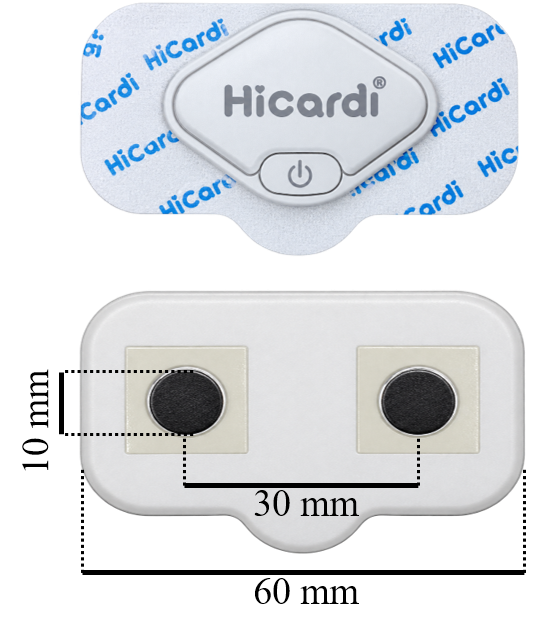
\includegraphics[height=80mm]{figures/impl_patch.png}\\[1.5mm]
  (a)
\end{minipage}%
\hfill
\begin{minipage}[b]{0.48\linewidth}
  \centering
  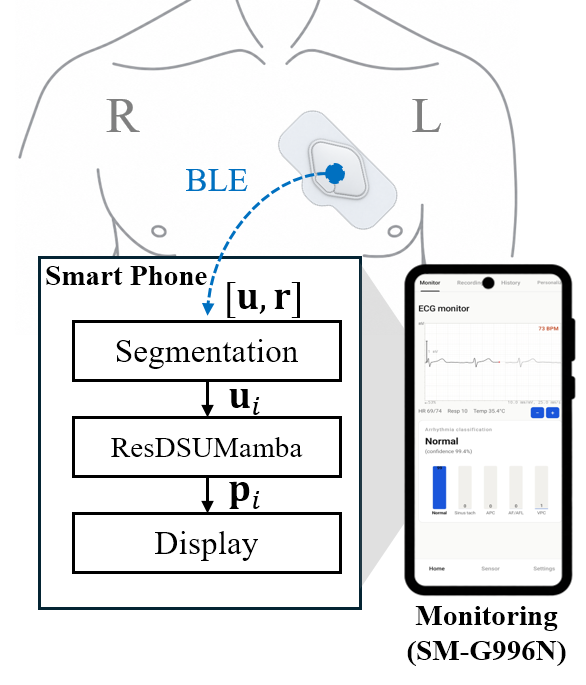
\includegraphics[height=80mm]{figures/impl_system.png}\\[1.5mm]
  (b)
\end{minipage}
\caption[HiCardi\textsuperscript{\textregistered} Smart Patch and system configuration.]{
HiCardi\textsuperscript{\textregistered} Smart Patch and system configuration.
(a) Patch and electrode geometry.
(b) ECG is streamed over BLE to the smartphone;
signal processing, beat classification, and display are performed on device.
}
\label{fig:impl_overview}
\end{figure}
The ResDSUMamba deployed in Chapter~3 was integrated into a smartphone application that continuously receives single-lead ECG from the HiCardi\textsuperscript{\textregistered} Smart Patch and processes the signal on a beat-by-beat basis.
In this work, real-time processing means continuously constructing beat-level inputs from the incoming ECG stream and performing inference and generating results for each beat in sequence.
As shown in Fig.~\ref{fig:impl_overview}, the ECG is transmitted from the patch to the smartphone via BLE, while signal reconstruction, R-peak alignment, input construction, classification, and result display are all handled on the device.
Fig.~\ref{fig:ble_spec} shows the BLE notification frame structure and ECG sample encoding, and Fig.~\ref{fig:impl_beat} illustrates the smartphone processing flow from received samples to beat-level classification.

% ====================================================
\section{ECG Data Acquisition}
% ====================================================

The HiCardi\textsuperscript{\textregistered} Smart Patch (MEZOO Co., Ltd., Wonju, Republic of Korea) transmits ECG through the Nordic UART Service (NUS)~\cite{nus}.
At the start of acquisition, the smartphone sequentially sends start commands using the write-without-response operation, without waiting for responses.
The patch then periodically transmits 42-byte notifications.
Fig.~\ref{fig:ble_spec} shows the notification frame structure and ECG sample encoding.
\begin{figure}[t]
\centering
% fig_impl_ble.tex
% BLE frame structure and ECG sample encoding.

\providecolor{bleblue}{RGB}{0,112,192}

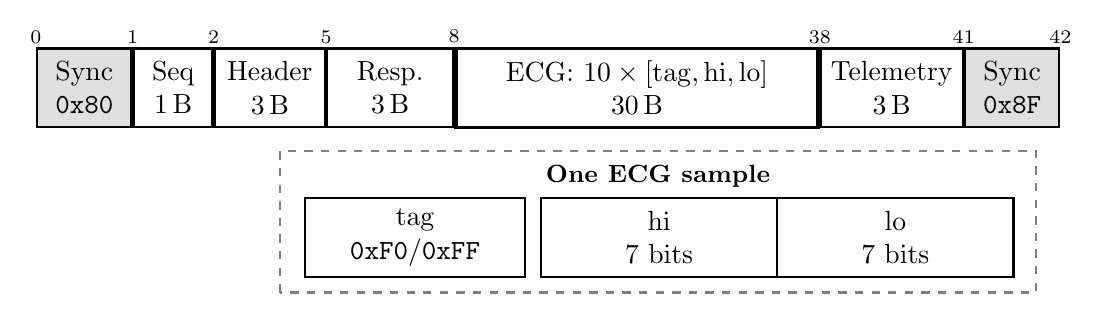
\begin{tikzpicture}[
  >=Stealth,
  thick,
  x=1mm,
  y=1mm,
  font=\rmfamily,
  cell/.style={
    draw,
    thick,
    minimum height=10mm,
    align=center,
    inner sep=1pt,
    anchor=west,
    font=\rmfamily
  },
  sync/.style={
    cell,
    fill=gray!25
  },
  sample/.style={
    draw,
    thick,
    minimum height=10mm,
    align=center,
    inner sep=2pt,
    anchor=west,
    font=\rmfamily
  },
  label/.style={
    anchor=south,
    font=\rmfamily\bfseries\small
  },
  off/.style={
    anchor=south,
    inner sep=1pt,
    font=\rmfamily\scriptsize
  },
  box/.style={
    draw=gray,
    thick,
    dashed,
    inner sep=3mm
  }
]

% 42-byte notification frame
\node[sync, minimum width=12mm] (c0) at (0,0)
  {Sync\\\texttt{0x80}};
\node[cell, minimum width=10mm] (c1) at (c0.east)
  {Seq\\1\,B};
\node[cell, minimum width=14mm] (c2) at (c1.east)
  {Header\\3\,B};
\node[cell, minimum width=16mm] (c3) at (c2.east)
  {Resp.\\3\,B};
\node[cell, minimum width=46mm, very thick] (c4) at (c3.east)
  {ECG: $10\times[\mathrm{tag},\mathrm{hi},\mathrm{lo}]$\\30\,B};
\node[cell, minimum width=18mm] (c5) at (c4.east)
  {Telemetry\\3\,B};
\node[sync, minimum width=12mm] (c6) at (c5.east)
  {Sync\\\texttt{0x8F}};

% Byte offsets
\foreach \c/\o in {
  c0/0,
  c1/1,
  c2/2,
  c3/5,
  c4/8,
  c5/38,
  c6/41
}{
  \node[off] at (\c.north west) {\o};
}
\node[off] at (c6.north east) {42};

% One ECG sample
\node[sample, minimum width=28mm] (tag) at (34,-19)
  {tag\\\texttt{0xF0}/\texttt{0xFF}};
\node[sample, minimum width=30mm] (hi) at (64,-19)
  {hi\\7 bits};
\node[sample, minimum width=30mm] (lo) at (94,-19)
  {lo\\7 bits};

% 점선 회색 박스와 라벨
\draw[box] (31,-26) rectangle (127,-8);
\node[label] at (79,-14) {One ECG sample};

\end{tikzpicture}
\caption[BLE frame structure and ECG sample encoding.]{
BLE frame structure and ECG sample encoding.
Each 42-byte notification contains 10 ECG samples represented by
\texttt{[tag, hi, lo]}, where \texttt{hi} and \texttt{lo} are 7-bit fields.
}
\label{fig:ble_spec}
\end{figure}
The ECG payload is organized into 3-byte groups in the form \texttt{[tag, hi, lo]},
and each 42-byte notification contains 10 ECG samples.
Only groups with a valid ECG tag are used to reconstruct the samples.
The two 7-bit fields, \texttt{hi} and \texttt{lo}, are then combined to obtain the 14-bit ADC value:
\begin{equation}
v=(\texttt{hi}\,\&\,\texttt{0x7F})\,2^7+(\texttt{lo}\,\&\,\texttt{0x7F}).
\label{eq:ble_decode}
\end{equation}
The reconstructed ADC value is converted to mV using $x=(v-8192)/1000$,
and the resulting signal, which uses the same scale as the training data, is fed to the model.
Sample validity is continuously monitored based on the signal-quality conditions.
Lead-off status is determined from the configured damaged-sample ratio and consecutive-frame criteria.
During lead-off periods, the ECG waveform continues to be displayed and recorded,
while R-peak tracking and inference states are updated accordingly.
The signal time axis is generated from sample indices rather than BLE notification arrival times,
using a sampling frequency of $f_s=250\,\mathrm{Hz}$.
RR intervals are then calculated from the difference in sample indices between consecutive R-peaks,
and packet sequence information is used to track the reception order and identify periods of packet loss.
 
% ====================================================
\section{On-Device Processing}
\label{sec:impl_pipeline}
% ====================================================
\begin{figure}[t]
\centering
\providecolor{bleblue}{RGB}{0,112,192}
\usetikzlibrary{arrows.meta}

\begin{tikzpicture}[
  x=1mm,
  y=1mm,
  font=\rmfamily,
  >={Bar[width=0.8pt] Triangle[length=3pt,width=4pt]},
  blk/.style={
    draw, 
    thick, 
    align=center, 
    text width=32mm,
    minimum height=14mm, 
    inner sep=1.5pt, 
    anchor=north, 
    font=\rmfamily
  },
  head/.style={
    align=center, 
    anchor=north, 
    font=\rmfamily\bfseries
  },
  arr/.style={
    ->, 
    thick
  },
  ble/.style={
    ->, 
    thick, 
    densely dashed, 
    bleblue
  }
]

  % ==================================================
  % Headers
  % ==================================================
  \node[head] at (19, 0)  {BLE Callback};
  \node[head] at (57, 0)  {Receive};
  \node[head] at (95, 0)  {Inference};

  % ==================================================
  % BLE Callback
  % ==================================================
  \node[blk] (a1) at (19,-10) {Frame Check};
  \node[blk] (a2) at (19,-28) {ECG Decode\\{\scriptsize 14-bit samples}};
  \node[blk] (a3) at (19,-46) {Lead-off Detection};

  % ==================================================
  % Receive
  % ==================================================
  \node[blk] (b1) at (57,-10) {R-Flag Reception};
  \node[blk] (b2) at (57,-28) {R-Peak Alignment\\{\scriptsize Past buffer search}};
  \node[blk] (b3) at (57,-46) {Heart Rate Update};

  % ==================================================
  % Inference
  % ==================================================
  \node[blk] (c1) at (95,-10) {Ring Buffer};
  \node[blk] (c2) at (95,-28) {Beat Windowing\\{\scriptsize $r_k \pm 250$ samples}};
  \node[blk] (c3) at (95,-46) {ResDSUMamba\\{\scriptsize Classification}};
  \node[blk] (c4) at (95,-64) {Post-processing\\{\scriptsize Threshold}};

  % ==================================================
  % UI
  % ==================================================
  \node[head] at (19,-84) {UI};
  \node[blk] (d1) at (57,-84) {ECG Waveform\\{\scriptsize Real-time sweep}};
  \node[blk] (d2) at (95,-84) {Display Results\\{\scriptsize HR \& Labels}};

  % ==================================================
  % BLE input
  % ==================================================
  \draw[ble] (19,-5.7) -- (a1.north);
  \node[anchor=west, font=\rmfamily\scriptsize] at (18,-6.5) {BLE};

  % ==================================================
  % Internal flows 
  % ==================================================
  \foreach \s/\t in {a1/a2, a2/a3, b1/b2, b2/b3, c1/c2, c2/c3, c3/c4} 
    \draw[arr] (\s.south) -- (\t.north);

  % ==================================================
  % Cross-column flows
  % ==================================================
  \draw[arr] (a2.east) -- (36.5,-35) -- (36.5,-17) -- (b1.west);
  \draw[arr] (b2.east) -- (74.5,-35) -- (74.5,-17) -- (c1.west);

  % ==================================================
  % UI flows
  % ==================================================
  \draw[arr] (b3.south) -- (d1.north);
  \draw[arr] (c4.south) -- (d2.north);

  % ==================================================
  % Separators
  % ==================================================
  \foreach \x in {38, 76}
    \draw[gray!55, densely dashed, thin] (\x, 8) -- (\x, -75);

  \draw[gray!55, densely dashed, thin] (0, -78) -- (113, -78);

\end{tikzpicture}
\caption[End-to-end on-device beat processing.]{
End-to-end on-device beat processing.
The pipeline is divided into four smartphone-side execution contexts:
the BLE callback, receive executor, inference executor, and UI thread.
Each block denotes a processing operation, and the queue between the receive
and inference executors provides thread-safe beat transfer.
}
\label{fig:impl_beat}
\end{figure}
 
As shown in Fig.~\ref{fig:impl_beat}, smartphone-side processing is divided among a BLE callback, a receive executor, an inference executor, and a UI thread.
The BLE callback validates incoming frames and reconstructs the ECG samples.
The receive executor handles R-peak alignment and other beat-related processing, while the inference executor constructs beat inputs, computes clinical features, and runs ResDSUMamba.
Meanwhile, the UI thread continuously updates the ECG waveform and classification results.
The receive and inference executors each run on a single thread, with a thread-safe queue used to pass beats from the receive executor to the inference executor.
 
Reconstructed ECG samples are stored in a fixed-size circular buffer together with their sample indices.
For each confirmed R-peak at sample index $n_k$, a 501-sample beat window $[n_k-W_{\mathrm{pre}},\,n_k+W_{\mathrm{post}}]$ is constructed with $W_{\mathrm{pre}}=W_{\mathrm{post}}=250$ samples, that is, $1.0\,\mathrm{s}$ on each side at $f_s=250\,\mathrm{Hz}$.
 
The patch provides an R-peak tag for each detected beat, but the tag is temporally offset from the corresponding R-peak in the ECG waveform.
Therefore, the tagged sample index is not used directly as the R-peak position.
Instead, the receive executor searches the preceding ECG segment and refines the R-peak location from the waveform, with a minimum interval of $240\,\mathrm{ms}$ between consecutive R-peaks.
The observed tag-to-waveform offset was approximately $\Delta_{\mathrm{tag}}=340\,\mathrm{ms}$, and this correction was applied consistently throughout the implementation.
% In a validation recording, this correction preserved all 64 detected beats and placed every refined R-peak within $\pm60\,\mathrm{ms}$ of the reference, with a median alignment error of $+2\,\mathrm{ms}$ and no duplicate detections.
This offset represents tag-to-waveform alignment rather than BLE notification transport latency.
 
The prepared beat is then passed to ResDSUMamba together with the patient embedding $\mathbf{p}\in\mathbb{R}^{256}$ and the clinical feature vector $\mathbf{c}\in\mathbb{R}^{32}$.
The patient embedding is obtained from the subject's initial $60\,\mathrm{s}$ baseline ECG using the CPC encoder.
Because the beat window extends $W_{\mathrm{post}}$ samples beyond the current R-peak, and the clinical features include the post-RR interval, inference can begin only after both the required future ECG samples and the subsequent R-peak are available.
 
Measured from the R-peak $n_k$, the time until the input of beat $k$ becomes available is therefore set by whichever condition is met later:
\begin{equation}
D_k =
\max\left(
RR_k^{\mathrm{post}}+\Delta_{\mathrm{tag}},\;
\frac{W_{\mathrm{post}}}{f_s}
\right),
\label{eq:input_wait}
\end{equation}
where $RR_k^{\mathrm{post}}$ is the interval between the current and subsequent R-peaks.
The first term is the time until the tag of the next R-peak arrives, and the second term is the time until the $W_{\mathrm{post}}$ post-peak samples are buffered, which is $250/250\,\mathrm{Hz}=1.0\,\mathrm{s}$.
At the mean heart rate of the live session in Section~\ref{sec:exp_live} ($80.2\,\mathrm{bpm}$, so $RR\approx748\,\mathrm{ms}$), the first term is about $748+340=1088\,\mathrm{ms}$, so $D_k\approx1.09\,\mathrm{s}$.
This delay is determined by the input definition and the tag offset, not by computation, and the beat-level processing time is added to it before a result is displayed.
Chapter~\ref{ch:experiments} evaluates whether beats are processed without backlog once their inputs are available; $D_k$ itself is derived here analytically and is not measured separately.
 %%%%%%%%%%%%%%%%%%%%%%%%%%%%%%%%%%%%%%%%%%%%%%%%%%%%%
% Chapter 5. Experiment
%%%%%%%%%%%%%%%%%%%%%%%%%%%%%%%%%%%%%%%%%%%%%%%%%%%%%
\chapter{Experiments}
\label{ch:experiments}

\section{Experimental Setup}

\subsection{Real-World Wearable ECG Dataset}
\label{sec:exp_dataset}

\begin{table}[!ht]
\centering
\caption{Cohort composition of the HiCardi records.}
\label{tab:hicardi_cohorts}
\resizebox{\textwidth}{!}{%
\begin{tabular}{llrrrrr}
\toprule
& & \multicolumn{3}{c}{Records} & & \\
\cmidrule(lr){3-5}
Cohort & Site & Train & Val. & Test & Records & Beats \\
\midrule
01 & Local Clinic & 42 & 11 & 45 & 98 & 5{,}744{,}567 \\
02 & Kosin & 11 & 6 & 23 & 40 & 3{,}137{,}371 \\
03 & Yonsei Resp.\ Env. & 12 & 3 & 26 & 41 & 3{,}867{,}625 \\
04 & Yonsei Resp.\ Env.\ 2022a & 20 & 3 & 23 & 46 & 3{,}638{,}596 \\
05 & Yonsei Resp.\ Env.\ 2022c & 17 & 4 & 21 & 42 & 2{,}222{,}122 \\
06 & Kosin ESKD & 17 & 12 & 21 & 50 & 913{,}321 \\
\midrule
\multicolumn{2}{l}{Total} & 119 & 39 & 159 & 317 & 19{,}523{,}602 \\
\bottomrule
\end{tabular}}
\normalsize
\end{table}

The HiCardi dataset consists of long-term ECG recordings collected using the
HiCardi Smart Patch and includes signal characteristics commonly
encountered in real-world wearable monitoring, such as motion artifacts,
signal loss, and changes in electrode contact.
The single-channel ECG was sampled at $250\,\mathrm{Hz}$, with recording
durations ranging from $0.03$ to $47.5$ hours.
The dataset contains $317$ records from $6$ cohorts used for training, validation, and evaluation after applying the calibration and signal-quality criteria.
Table~\ref{tab:hicardi_cohorts} summarizes the composition of each cohort,
which are grouped according to acquisition site and recording period.

The five evaluation labels are Normal, APC, VPC, sinus tachycardia, and AF/AFL.
APC and VPC represent beat-level morphological labels, whereas sinus
tachycardia and AF/AFL represent interval-level rhythm labels.
Because a beat can have more than one label, the task was formulated as a
multi-label classification problem.
Normal denotes a normal heartbeat and was included as a reference label.
The initial $60\,\mathrm{s}$ of each subject was used only as an unlabeled
baseline segment for patient-embedding extraction and was excluded from
performance evaluation.

Table~\ref{tab:hicardi_cohorts} reports record counts after the cohort-level
inclusion criteria, giving $159$ test records. Of these, $21$ records did not
contain a calibration segment that met the length and signal-quality
requirements used for patient-embedding extraction (the initial unlabeled
$60\,\mathrm{s}$ segment described above) and were excluded from the
record-level evaluation that follows, leaving $138$ evaluation records.

The training, validation, and evaluation data were divided at the record level.
Among the $78$ subjects contributing beats to the evaluation set, $27$ also had
recordings from different days included in the training data.
These overlapping subjects accounted for $87$ of the $138$ evaluation records
and $6{,}146{,}182$ of the $8{,}777{,}480$ evaluation beats
($70.0\,\%$).

\subsection{Target Device and Measurement} 
\label{sec:exp_devices}

Device measurements were performed on a Samsung SM-G996N (Exynos 2100, arm64-v8a, 8 CPU cores, Android 15, SDK 35).
The deployed model used the FP32 XNNPACK configuration of ExecuTorch, batch size 1, and one worker thread.
Inference was executed on a Cortex-X1 core using a single thread.
The operating frequency was not fixed, and other threads in the actual system handled BLE reception, buffer management, and screen updates.
In the deployed graph, operations supported by XNNPACK were delegated to the XNNPACK backend, while unsupported operations were executed by the ExecuTorch portable kernel.
The Portable and XNNPACK configurations were compared.
$T_{\mathrm{model}}$ was measured after 100 warm-up iterations by executing 2,000 forward passes and recording the CPU time used by the inference thread during each forward pass.
The mean (Avg), $P5$, $P50$, and $P95$ were all calculated from these 2,000 samples.
Peak Native Heap denotes the maximum native allocation observed for the application process during the measurement session.

\subsection{Evaluation Metrics}
\label{sec:timing_metrics}

The measurements in Section~\ref{sec:exp_devices} were obtained by repeatedly executing the model with the input already prepared. During actual streaming, ECG reception, R-peak correction, and inference operate concurrently; therefore, processing time is measured separately for each beat within the application. This work distinguishes the following three timing metrics.
\begin{itemize}
\item $T_{\mathrm{model}}$: CPU execution time of one model forward pass given a prepared input, as measured in Section~\ref{sec:exp_devices}.
\item $T_{\mathrm{queue}}$: wall-clock waiting time from the moment the beat input becomes ready until the inference executor begins processing it.
\item $T_{\mathrm{beat}}$: total wall-clock elapsed time from input readiness until the corresponding beat-processing result is generated. This includes input construction, feature computation, model execution, and post-processing.
\end{itemize}

For beat $k$, the input-ready time $t^{\mathrm{ready}}_k$, the actual processing start time of the inference executor $t^{\mathrm{start}}_k$, and the result-generation time $t^{\mathrm{end}}_k$ are recorded using a monotonic clock. The metrics are calculated as
\begin{equation}
T_{\mathrm{queue},k}
=
t^{\mathrm{start}}_k - t^{\mathrm{ready}}_k,
\qquad
T_{\mathrm{beat},k}
=
t^{\mathrm{end}}_k - t^{\mathrm{ready}}_k.
\label{eq:tbeat}
\end{equation}
$T_{\mathrm{queue}}$ and $T_{\mathrm{beat}}$ are wall-clock times, whereas $T_{\mathrm{model}}$ is CPU time. $T_{\mathrm{beat}}$ includes input construction, feature computation, model execution, and post-processing.

Real-time streaming in this work is evaluated as the capability to continuously process sequential beat-level inputs rather than as a measure of end-to-end clinical decision latency. The next beat input typically becomes ready after an interval determined by the subsequent R-peak and the required post-peak samples. Accordingly, sustained operation without backlog requires the beat-processing workload to remain within the available inter-beat processing interval. When beats accumulate, the waiting time $T_{\mathrm{queue}}$ increases. Therefore, whether $T_{\mathrm{queue}}$ continues to increase throughout the session is also monitored. In this work, $T_{\mathrm{queue}}$ is reported only as its maximum value over a session (Section~\ref{sec:exp_live}); no within-session time series is plotted, so a gradual upward trend could not be distinguished from occasional spikes using the reported statistic alone.

CPU utilization of the process and major threads and memory usage are recorded at $1\,\mathrm{Hz}$. Each measurement session is logged together with the model file, runtime, backend, numerical precision, batch size, and thread count. The measurement logs are written to a file by a separate logging thread that dequeues records without blocking ECG reception or inference. During measurement, automatic screen-off was disabled to maintain consistent execution conditions.

Because the HiCardi dataset is multi-label, each label is treated as an independent binary classification problem. For each label, Accuracy (Acc), Sensitivity (Se), Specificity (Sp), positive predictivity (P+), and $F_1$ are calculated. A label is predicted as positive when its output probability is at least $0.5$. Macro metrics are obtained by averaging the metric values of the five labels (Normal, APC, VPC, sinus tachycardia, and AF/AFL) with equal weights. Micro metrics are computed after aggregating the TP, FP, FN, and TN counts across all five labels.


\section{Experimental Results}

\subsection{Arrhythmia Classification Performance} 
\label{sec:classification_perf}

\begin{table}[h]
\centering
\caption[Classification performance on the HiCardi test set.]{Classification performance (\%) on the HiCardi test set.}
\label{tab:hicardi_main}
\setlength{\tabcolsep}{4.35pt}
\small
\begin{tabular}{@{}lcccccccccc@{}}
\toprule
& \multicolumn{5}{c}{Macro} & \multicolumn{5}{c}{Micro} \\
\cmidrule(lr){2-6}\cmidrule(lr){7-11}
Model & Acc. & Se & Sp & P+ & $F_1$ & Acc. & Se & Sp & P+ & $F_1$ \\
\midrule
ResUMamba & 91.71 & 78.00 & 93.66 & 39.21 & 42.28 & 91.71 & 79.21 & 94.83 & 79.32 & 79.27 \\
ResDSUMamba & 93.32 & 75.72 & 94.32 & 41.67 & 44.15 & 93.32 & 83.21 & 95.85 & 83.37 & 83.29 \\
\bottomrule
\end{tabular}
\end{table}

Table~\ref{tab:hicardi_main} compares the classification performance of ResUMamba and ResDSUMamba on the HiCardi test set using a record-wise split.
The split was configured so that unique record identifiers did not overlap between the training and test sets.
The Macro-$F_1$ and Micro-$F_1$ values of ResUMamba were $42.28\%$ and $79.27\%$, respectively,
while those of ResDSUMamba were $44.15\%$ and $83.29\%$, respectively.
The differences between the two models were $1.87$ percentage points in Macro-$F_1$ and $4.02$ percentage points in Micro-$F_1$.
Macro-Se was $78.00\%$ for ResUMamba and $75.72\%$ for ResDSUMamba.

\subsection{Effect of Software Optimization on Mobile CPU Time}
\label{sec:exp_backend}

\begin{table}[h]
\centering
\caption[Model execution time under Portable and XNNPACK configurations.]{%
$T_{\mathrm{model}}$ (ms) on Samsung SM-G996N (Exynos 2100) under Portable and XNNPACK configurations.}
\label{tab:delegation_scope}
\footnotesize
\setlength{\tabcolsep}{2.2pt}
\resizebox{\textwidth}{!}{%
\begin{tabular}{@{}lrrrrrrrrrr@{}}
\toprule
& \multicolumn{5}{c}{ResUMamba} & \multicolumn{5}{c}{ResDSUMamba} \\
\cmidrule(lr){2-6}\cmidrule(lr){7-11}
Backend & Avg & $P5$ & $P50$ & $P95$ & $\Delta$Avg
& Avg & $P5$ & $P50$ & $P95$ & $\Delta$Avg \\
\midrule
Portable
& 1073.57 & 869.08 & 1211.25 & 1240.56 & 0
& 611.50 & 537.09 & 549.20 & 767.10 & 0 \\
XNNPACK
& 48.25 & 46.56 & 47.77 & 51.71 & 1025.33
& \textbf{36.70} & \textbf{35.59} & \textbf{36.11} & \textbf{38.90} & 574.80 \\
\bottomrule
\end{tabular}}
\end{table}

Table~\ref{tab:delegation_scope} compares the CPU execution time of one prepared
beat input, $T_{\mathrm{model}}$, under two software execution configurations:
the ExecuTorch portable-kernel configuration and the XNNPACK configuration.
In the portable configuration, model operators are executed using ExecuTorch
portable kernels, whereas operations supported by XNNPACK are delegated to the
XNNPACK backend in the XNNPACK configuration.

For ResUMamba, the mean $T_{\mathrm{model}}$ decreased from
$1073.57\,\mathrm{ms}$ with the portable configuration to
$48.25\,\mathrm{ms}$ with XNNPACK, corresponding to a reduction of $95.5\%$.
For ResDSUMamba, the mean decreased from $611.50\,\mathrm{ms}$ to
$36.70\,\mathrm{ms}$, corresponding to a reduction of $94.0\%$.
Under XNNPACK, ResDSUMamba was additionally $11.55\,\mathrm{ms}$
faster than ResUMamba, corresponding to a relative reduction of $23.9\%$.
The $P95$ of ResDSUMamba was $38.90\,\mathrm{ms}$.

These results show that the software execution configuration had a substantial
effect on mobile CPU inference time. The large reduction from the portable
configuration to XNNPACK was observed for both models, while the additional
use of DSConv further reduced the execution time under the XNNPACK
configuration.

\subsection{Real-World Live Wearable Patch Evaluation}
\label{sec:exp_live}

A single session lasting $309.21\,\mathrm{s}$ (approximately 5~min 9~s)
was measured while the patch was attached and connected to the smartphone via BLE.
The final deployment configuration was evaluated under actual streaming conditions,
including ECG reception, R-peak alignment, beat construction, inference, and
screen updates.
During the measurement, the application performed ECG reception, R-peak alignment,
beat classification, and screen updates.
The definitions of the timing and resource metrics and the logging procedure are described in Section~\ref{sec:timing_metrics}.

\begin{figure}[t]
\centering
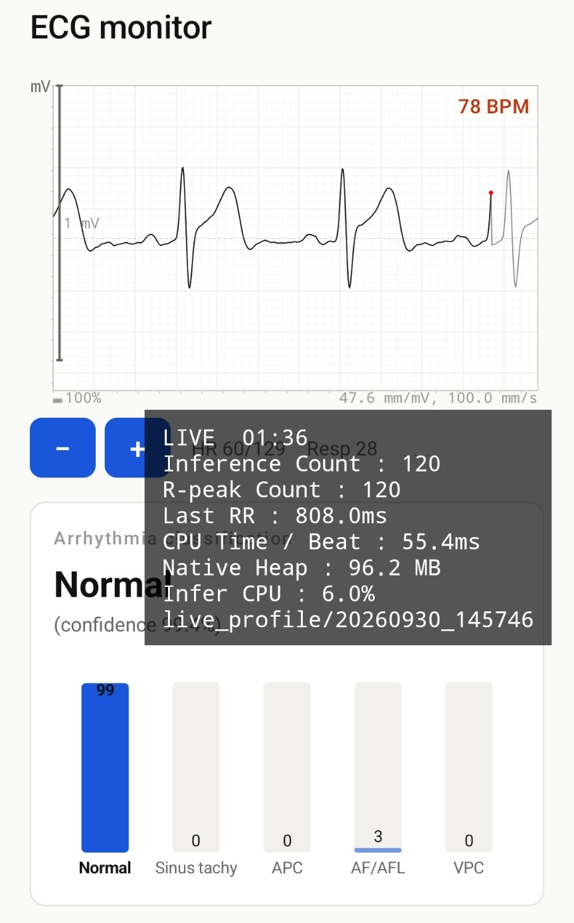
\includegraphics[width=0.6\textwidth]{figures/live_profiler.png}
\caption[Resource usage during live ECG streaming.]{Resource usage during live ECG streaming with the HiCardi patch:
Monitor screen with the CPU and memory traces recorded on the target device.}
\label{fig:live_profile}
\end{figure}

Fig.~\ref{fig:live_profile} shows the Monitor screen together with CPU and memory utilization during the measurement period.
The CPU utilization of the inference thread was $7.9\%$, that of the reception thread was $1.0\%$, and Peak Native Heap was $99.2\,\mathrm{MB}$.
A total of $413$ beats were recorded during the session.
Using the measured session duration of $309.2056\,\mathrm{s}$, the beat rate was
$413/309.2056\times60=80.14\,\mathrm{bpm}$.
The mean heart rate reported by the application was $80.2\,\mathrm{bpm}$.
$T_{\mathrm{beat}}$ was $59.4\,\mathrm{ms}$ on average,
with a $P50$ of $56.9\,\mathrm{ms}$ and a $P95$ of $70.3\,\mathrm{ms}$.
The maximum $T_{\mathrm{queue}}$ was $11.4\,\mathrm{ms}$.
All beats were classified as Normal.

\begin{table}[t]
\centering
\caption[Resource usage during continuous ECG streaming.]{Resource usage during continuous ECG streaming with the HiCardi patch on Samsung SM-G996N (Exynos 2100).}
\label{tab:live_profile}
\small
\begin{tabular}{@{}llr@{}}
\toprule
Group & Metric & Value \\
\midrule
\multirow{3}{*}{Session}
& Duration & $309.21\,\mathrm{s}$ (approx. 5 min 9 s) \\
& Detected beats $N_{\mathrm{R}}$ & 413 \\
& Reported heart rate & $80.2\,\mathrm{bpm}$ \\
\midrule
\multirow{5}{*}{Processing}
& $T_{\mathrm{beat}}$ (Avg.) & $59.4\,\mathrm{ms}$ \\
& $T_{\mathrm{beat}}$ ($P5$) & $49.7\,\mathrm{ms}$ \\
& $T_{\mathrm{beat}}$ ($P50$) & $56.9\,\mathrm{ms}$ \\
& $T_{\mathrm{beat}}$ ($P95$) & $70.3\,\mathrm{ms}$ \\
& $T_{\mathrm{queue}}$ (max) & $11.4\,\mathrm{ms}$ \\
\midrule
\multirow{3}{*}{Resource}
& CPU, inference thread & $7.9\,\%$ \\
& CPU, receive thread & $1.0\,\%$ \\
% & CPU, process & $46.3\,\%$ \\
& Peak Native Heap & $99.2\,\mathrm{MB}$ \\
\bottomrule
\end{tabular}
\end{table}


%%%%%%%%%%%%%%%%%%%%%%%%%%%%%%%%%%%%%%%%%%%%%%%%%%%%%
% Chapter 6. Conclusion
%%%%%%%%%%%%%%%%%%%%%%%%%%%%%%%%%%%%%%%%%%%%%%%%%%%%%
\chapter{Conclusion} \label{ch:conclusion}
 
This work developed ResDSUMamba as a lightweight version of ResUMamba and implemented it as an on-device smartphone inference pipeline that classifies beats from a wearable ECG stream in real time.
The original ResUMamba combines a ResU path for extracting morphological ECG features with a Mamba path for modeling temporal dependencies.
For Android CPU deployment, this work uses a deployment-oriented sequential scan based on standard ATen operators and optimizes both the model architecture and its computational representation.
 
First, ResDSUMamba was constructed by replacing the standard one-dimensional convolutions in the ResU path with depthwise separable convolutions and retraining the resulting model under the same data split and classification objective.
The Mamba path uses the weights of the trained ResDSUMamba, and the selective scan is represented using a sequential scan composed of standard PyTorch operators before deployment through ExecuTorch.
For real-time execution, the ECG processing pipeline was implemented to handle ECG reception, 14-bit sample reconstruction, circular-buffer management, R-peak alignment, beat construction, and model inference.
Reception and inference were executed on separate threads.
Signal quality, lead-off status, and packet loss were monitored during reception, and R-peak tracking and inference states were updated accordingly.
 
ResDSUMamba reduced the number of parameters from $2.4883\,\mathrm{M}$ to $1.3225\,\mathrm{M}$, corresponding to a reduction of $46.9\%$, and reduced the number of MACs from $721.50\,\mathrm{M}$ to $331.38\,\mathrm{M}$, corresponding to a reduction of $54.1\%$.
On the HiCardi dataset using a record-wise split, the Macro-$F_1$ and Micro-$F_1$ values of ResUMamba were $42.28\%$ and $79.27\%$, respectively, whereas those of ResDSUMamba were $44.15\%$ and $83.29\%$.
The corresponding Macro-Se values were $78.00\%$ and $75.72\%$, so the gain in $F_1$ came with a lower average sensitivity across labels.
 
On the Galaxy~S21+, the mean $T_{\mathrm{model}}$ under the XNNPACK configuration was $48.25\,\mathrm{ms}$ for ResUMamba and $36.70\,\mathrm{ms}$ for ResDSUMamba.
Most of the reduction from the portable configuration came from XNNPACK delegation ($95.5\%$ for ResUMamba), and DSConv reduced the mean execution time by a further $11.55\,\mathrm{ms}$, corresponding to a relative reduction of $23.9\%$.
The $P95$ of ResDSUMamba was $38.90\,\mathrm{ms}$.
 
During actual HiCardi patch streaming, $413$ beats were processed over $309.21\,\mathrm{s}$, and the application reported a mean heart rate of $80.2\,\mathrm{bpm}$.
$T_{\mathrm{beat}}$ was $59.4\,\mathrm{ms}$ on average, with a $P95$ of $70.3\,\mathrm{ms}$, and the maximum $T_{\mathrm{queue}}$ was $11.4\,\mathrm{ms}$.
The CPU utilization of the inference thread was $7.9\%$, and Peak Native Heap was $99.2\,\mathrm{MB}$.
These results show that the on-device streaming pipeline was able to process wearable patch ECG on the smartphone on a beat-by-beat basis without backlog under the measurement conditions used in this study.
 
%% =================================================
\section{Limitations and Future Work} \label{sec:conclusion_limitations}
 
The on-device evaluation in this work was conducted in a single $309.21\,\mathrm{s}$ session on a Galaxy~S21+.
Although $T_{\mathrm{model}}$ and $T_{\mathrm{beat}}$ were measured, the input-availability delay of about $1.09\,\mathrm{s}$ was derived analytically, and end-to-end latency including BLE communication and screen rendering, power consumption, and thermal behavior during prolonged operation were not evaluated.
Future work will extend the evaluation to a wider range of heart-rate conditions, longer-duration measurements, and multiple mobile devices.
 
The live session did not include synchronized clinical ground-truth labels, and all beats in the session were classified as Normal.
In this setting, processing time and resource usage were measured, but classification performance could not be directly evaluated against clinical annotations.
Future work will compare the deployed model with physician annotations from actual arrhythmia patients.
 
The HiCardi dataset is not publicly available to protect patient privacy.
However, access may be granted for academic and research purposes through the predefined approval procedures established by the data management authority.

Numerical agreement between the PyTorch training-time model and its ExecuTorch-exported graph was not verified. The classification performance in Table~\ref{tab:hicardi_main} is measured on the PyTorch model, and the on-device timing in Table~\ref{tab:delegation_scope} and Table~\ref{tab:live_profile} is measured on the exported graph; the two are not linked by a reported output-parity check, so the exported graph's classification performance is assumed, not demonstrated, to match Table~\ref{tab:hicardi_main}.
\clearpage
